\documentclass[a4paper,12pt]{article}


\usepackage{amsmath}
\usepackage{graphicx}
\usepackage[capposition=bottom]{floatrow}
\usepackage{amssymb}
\usepackage{subfig}
\usepackage{graphicx}
\usepackage{caption}
\usepackage{rotating}
\usepackage{hyperref}

\linespread{2}
\def\mean#1{\left< #1 \right>}
\begin{document}
\title{Thesis Intro}
\author{Richard Knoche}
\maketitle

\tableofcontents

\section{Introduction to Dark Matter}

In recent decades it has been discovered that the luminous matter which scientists have studied for centuries is only a small fraction of the total composition of the universe.  There is strong evidence of dark baryonic matter (a few percent), nonbaryonic hot dark matter ($\sim$0.1\%-1.5\%), non baryonic cold dark matter ($\sim$25\%), and dark energy ($\sim$70\%) components to the universe, where the percentages are as a total fraction of their contribution to the universe's total composition.  While we know a large amount about the ``normal" matter which contributes $ \lesssim $ 4\% of the universe's total composition, we know very little about these larger components.  In particular, while we understand certain characteristics of the cold dark matter component, there is no consensus on its composition.  Before examining the experiments which seek to answer this question we will first discuss what is currently known about the nonbaryonic dark matter component.

\subsection{Evidence for Dark Matter}

\subsubsection{Mass Measurements from Galactic Rotation Curves}

In the early 1930's Fritz Zwicky was the first to use the Virial theorem to determine the total mass of the Coma cluster of galaxies.   measured the rotational velocity of eight galaxies in the Coma Cluster. In his examination, Zwicky found that the velocities at large radii were too high to be consistent with the Newtonian prediction arising from the visible matter alone \cite{Zwicky}. This discrepancy was reinforced in the 1970's, when further data on the rotational velocity of spiral galaxies began to be collected.  Instead of the rotational velocity falling off as $\propto 1/\sqrt{r}$ beyond the radius of visible matter as one would expect, the rotational velocity rises for small radii, then asymptotes to a constant $ v \simeq 100-300 \; km/s $ for large radii in most galaxies \cite{Persic,Battaner,Binney}.  The most widely accepted explanation of this phenomenon is that the disk galaxies are immersed in a dark matter (DM) halo such that $ M(r)/r $ remains constant at large radii.  Such a halo could form from a self gravitating ball of ideal gas at a uniform temperature.

\begin{center}
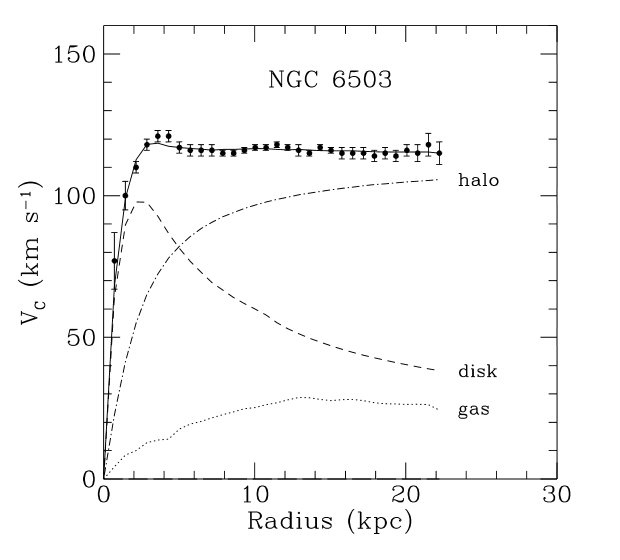
\includegraphics[scale=.7]{RotationCurve2.png}
\captionof{figure}{Rotation curve of galaxy NGC 6503.  The dotted line indicates the contribution of baryonic gas, the dashed line indicates the contribution of visible matter in the disk, and the dash-dotted line indicates the contribution of dark matter.  In the absence of dark matter the total velocity curve would fall off in a manner similar to the dotted line.\cite{Begeman}}
\end{center}


Following Zwicky's footsteps, we can use the Virial theorem to calculate the luminous matter's contribution to the total mass of the Coma Cluster.  The theorem states that for a system of $N$ particles
\begin{equation} \label{VirialTheorem}
\frac{1}{2} \sum_{i=1}^{N} \langle m_i v^2_i \rangle = -\frac{1}{2} \sum_{i=1}^N \langle \mathbf{r}_i \cdot {\mathbf{F}_i} \rangle
\end{equation} \label{VirialTheorem2}
where $m_i$,$v_i$, and $\mathbf{r}_i$ are the mass, velocity, and position of the $i$th particle in a system of particles, and $\mathbf{F}_i$ is the force acting on the same particle.  Since the total force on a particle is the sum of all of the forces acting on it
\begin{equation}
\mathbf{F}_i = \sum_{j=1}^N \mathbf{F}_{ji}
\end{equation} \label{VirialTheorem3}
where $\mathbf{F}_{ji}$ is the force that particle $j$ applies on particle $i$.  Noting that a particle does not apply force to itself, and that Newton's third law of motion states that $\mathbf{F}_{ji} = -\mathbf{F}_{ij}$ we can rewrite the right hand side of the Virial theorem to be
\begin{equation} \label{VirialTheorem4}
 \sum_{i=1}^N \mathbf{F}_i \cdot \mathbf{r}_i = \sum_{i=1}^N \sum_{j<i} \mathbf{F}_{ji} \cdot \mathbf{r}_i +  \sum_{i=1}^N \sum_{j>i} \mathbf{F}_{ji} \cdot \mathbf{r}_i = \sum_{i=1}^N \sum_{j<i} \mathbf{F}_{ji} \cdot (\mathbf{r}_i - \mathbf{r}_j).
 \end{equation}
Using the law of gravitation to apply equation \ref{VirialTheorem4} to a cluster of galaxies, the Virial theorem becomes
\begin{equation} \label{VirialTheorem5}
 \sum_{i=1}^{N} \langle m_i v^2_i \rangle = \sum_{i}^{N} \sum_{j<i} \langle  \frac{Gm_im_j}{r_{ij}} \rangle
 \end{equation}
where G is the gravitational constant.  The left hand side of this equation is the total mass, $M$, of the cluster of galaxies multiplied by the time and mass averaged squared velocity.  The right hand side is approximately equal to $\frac{GM^2}{R}$, where $R$ is the radius of the galaxy cluster.  Rearranging equation ??, we arrive at an equation which relates the total mass of the galaxy cluster to the mean square velocity
\begin{equation} \label{VirialTheorem6}
 M \approx \frac{ \langle v^2 \rangle R }{G}
\end{equation} 

The mean square velocity of a galaxy cluster can be estimated by calculating the one dimensional line of sight velocity via redshift.  Under the assumption of spherical symmetry
\begin{equation} \label{VirialTheorem7}
 \langle v^2 \rangle = 3 \langle (v_r - c \langle z \rangle)^2 \rangle
\end{equation} 
where $\langle z \rangle$ is the measured redshift of the galaxy cluster, $v_r$ is the line of sight velocity, and c is the speed of light.  For the Coma cluster $\langle z \rangle = 0.0232$, which produces an estimate of $\langle v^2 \rangle \approx 2 \times 10^{12} \frac{m^2}{s^2}$.\cite{ComaZ}  Using the measured radius of the Comma cluster ($R \approx 5 \times 10^{22}$) the total mass of the system in terms of solar mass ($M_{\odot}$) is found to be
\begin{equation} \label{VirialTheorem8}
M_{total} \approx 2 \times 10^{15} M_{\odot}.
\end{equation}
Comparing this the mass calculated from luminous matter alone we see that these components contribute only a small fraction of the total mass of the system. \cite{ComaZ}
\begin{equation} \label{VirialTheorem9}
\frac{M_{lum}}{M_{total}} \approx \frac{2.3 \times 10^{14} M_{\odot}}{2 \times 10^{15} M_{\odot}} = 0.11
\end{equation}

\subsubsection{Mass Measurements from x-ray Gases}

The total mass of a dynamically relaxed galaxy cluster can be measured from the hydrostatic equilibrium equation, which can be derived from the Tolman-Oppenheimer-Volkoff equation for stellar structure by taking the nonrelativistic  limit of $c \rightarrow \infty$, such that 
\begin{equation} \label{HEq1}
\frac{dP}{dr} = -\frac{GM(r)}{r^2}\rho
\end{equation}
where $P$ is the pressure of the gas in a cluster, $G$ is the gravitational constant, $M(r)$ is the mass of the galaxy cluster at a particular radius, and $\rho$ is the density of the gas in the cluster.  From the ideal gas law we know that
\begin{equation} \label{HEq2}
P=(\frac{\rho}{\mu m_H})kT
\end{equation}
where $\mu$ is the mean molecular weight ($\sim$0.6 for an ionized plasma), $m_H$ is the mass of the hydrogen atom, and k is Boltzman's constant.  Plugging this into equation \ref{HEq1} yields
\begin{equation} \label{HEq3}
(\frac{k}{\mu m_H})(T\frac{d\rho}{dr} + \rho\frac{dT}{dr})=-(\frac{GM(r)}{r^2})\rho
\end{equation}
Solving equation \ref{HEq3} for $M(r)$ produces a measurement of the cluster's mass from x-ray gas density and temperatures
\begin{equation} \label{HEq4}
M(r) = -\frac{kT}{\mu m_H G}(\frac{d \; ln(\rho)}{d \; ln(r)} + \frac{d \; ln(T)}{d \; ln(r)})r
\end{equation}
where the logarithms were introduced using the fact that $\frac{r}{t}\frac{dT}{dr}=\frac{\frac{dT}{T}}{\frac{dr}{r}}=\frac{ d \; ln{T}}{d \; ln{r} }$. 
This mass measurement technique is complicated by the fact that the gas density and temperature of a galaxy cluster has spatial variation, as well as the fact that x-ray emission measurements are a two-dimensional projection of a three-dimensional object, which  produces complications when integrating x-ray spectra along lines of sight through the cluster. One method for simplifying the mass measurement, called the beta model, is to assume the cluster is made of isothermal, spherically symmetric gas.  In this case the density of the gas traces the density of the gravitational mass, such that
\begin{equation} \label{HBeta1}
\rho_{gas}(r) = \rho_0(1 + \frac{r}{r_c})^{-3\beta/2}
\end{equation}
where $r_c$ is the core radius, $\rho_0$ is the central density, and $\beta$ is a slope parameter.  \cite{Vikhlinin}  The core radius $r_c$ is defined using the intensity of x-ray observations such that $I(r_c)=\frac{1}{2}I(0)$, or more generally to be the radius at which $\frac{d^2 \; ln(I)}{d \; ln(r)^2}$ is maximized. In this model the mass measurement reduces to a derivation of the spatial density profile by determining the best fit parameters of $r_c$ and $\beta$ to the x-ray observations.  When this mass measurement technique is compared to mass measurements from luminous matter alone more evidence for dark matter arises. For example, using this technique the Virgo Cluster has been measured to have a total mass (within r $<$ 1.8Mpc) between $1.5 \times 10^{14} M_{\odot}$ and $5.5 \times10^{14} M_{\odot}$. \cite{Paradijs} Comparing this to the mass measured from x-ray luminosity yields a ratio of
\begin{equation} \label{betamodelmass}
\frac{M_{lum}}{M_{total}} \approx \frac{4.75 \times 10^{13} M_{\odot}}{3.5 \times 10^{14} M_{\odot}} = 0.14
\end{equation}

\subsubsection{Gravitational Lensing}


Gravitational lensing provides an independent method for measuring the mass of galaxy clusters and other astronomical objects.  Gravitational lensing can be divided into two categories -- strong lensing and weak lensing.  Strong lensing, in which a background light source is distorted into arcs around a massive foreground object, is a rare phenomenon which requires a light source and a very massive lens to be nearly in line with the observer.  When such a situation occurs the mass of the lens can be inferred from the angular width of the arc of light which is produced.  We now turn to general relativity to derive the equation which produces this mass measurement.

The geodesic equation, which describes the path that a free particle travels, is given by
\begin{equation} \label{geodesic}
\frac{d}{d\tau}(g_{aj} \frac{dx^j}{d\tau})-\frac{1}{2}\frac{\partial g_{ij}}{\partial x^a} \frac{dx^i}{d\tau}\frac{dx^j}{d\tau} = 0
\end{equation}
where $g_{\alpha j}$ is a metric, $\tau$ is the proper time, and $x$ is the four dimensional coordinate vector. For a spacetime in a vacuum outside of a spherically symmetric mass the appropriate metric to use is the Schwarzschild metric.  With units of $c=1$ it is given by
\begin{equation} \label{s-metric}
ds^2 = -(1-\frac{2GM}{r})dt^2 + (1-\frac{2GM}{r})^{-1}dr^2+r^2 d \theta^2 + r^2 sin^2 \theta d\phi^2.
\end{equation}
From the $t$ component of the geodesic equation we know that
\begin{equation} \label{geodesic-t}
\frac{d}{d \tau}(g_{tj}\frac{dx^j}{d\tau}) - \frac{1}{2} \frac{\partial g_{ij}}{dt} \frac{dx^i}{d\tau} \frac{dx^j}{d \tau} =0.
\end{equation}
The Schwarzschild metric does not depend on time, and is diagonal, therefore
\begin{equation} \label{geodesic-t-reduced}
\frac{d}{d \tau}(g_{tj}\frac{dx^j}{d\tau}) = \frac{d}{d \tau}(g_{tt}\frac{dt}{d\tau}) = -\frac{d}{d \tau}((1-\frac{2GM}{r})\frac{dt}{d\tau}) = 0.
\end{equation}
Equation \ref{geodesic-t} is true if the quantity inside of the derivative is constant, leading us to the first constant of motion
\begin{equation}\label{first com}
E=(1-\frac{2GM}{r})\frac{dt}{d\tau}.
\end{equation}
We now turn to the $\phi$ component of the geodesic equation
\begin{equation} \label{geodesic-phi}
\frac{d}{d \tau}(g_{\phi j}\frac{dx^j}{d\tau}) = \frac{d}{d \tau}(g_{\phi \phi}\frac{d\phi}{d\tau}) = -\frac{d}{d \tau}(r^2 sin^2 \theta \frac{d\phi}{d\tau}) = 0
\end{equation}
where we have once again used the fact that the metric does not depend on time and is diagonal to simplify the equation.  From this we arrive at the second constant of motion
\begin{equation} \label{second com}
l=r^2sin^2\theta \frac{d\phi}{d \tau}
\end{equation}
%If we assume motion in the equatorial plane then $\theta=\pi/2$, and the ratio 
%of the two constants of motion becomes
%\begin{equation} \label{com ratio}
%u \equiv \frac{l}{E} = \frac{r^2\frac{d\phi}{d\tau}}{(1-\frac{2GM}{r})\frac{dt}{d\tau}}=(1-\frac{2GM}{r})^{-1} r^2 \frac{d\phi}{dt}
%\end{equation}
%From this we get the equation of motion
%\begin{equation} \label{phi eqm}
%\frac{d\phi}{dt} = \frac{1}{r^2}(1-\frac{2GM}{r})u
%\end{equation}
Returning to the Schwarzschild metric, for a photon $ds^2$=0, and if we assume motion in the equatorial plane $\theta=\pi/2$ and $d \theta =0$, such that
\begin{equation} \label{photon metric}
-(1-\frac{2GM}{r})dt^2 + (1-\frac{2GM}{r})^{-1}dr^2+r^2 d\phi^2=0.
\end{equation}
From the two constants of motion we know that
\begin{equation} \label{dphi}
d\phi^2=\frac{l^2}{r^4 sin^4 \theta} d\tau^2
\end{equation}
and
\begin{equation} \label{dt}
dt^2=E^2(1-\frac{2GM}{r})^{-2}d\tau^2
\end{equation}
Plugging equations \ref{dphi} and \ref{dt} into equation \ref{photon metric} and simplifying yields
\begin{equation} \label{dr2}
dr^2=[E^2 - (1-\frac{2GM}{r}) \frac{l^2}{r^2}]d\tau^2
\end{equation} 
Finally, by dividing equation \ref{dr2} by \ref{dphi} we arrive at the equation of motion for light traveling in a Schwarzschild spacetime in polar coordinates
\begin{equation} \label{polar eqm}
(\frac{1}{r^2} \frac{dr}{d \phi})^2 = (\frac{E}{l})^2 - (1-\frac{2GM}{r})\frac{1}{r^2} \equiv (\frac{1}{b})^2 - (1-\frac{2GM}{r})\frac{1}{r^2}
\end{equation}
The quantity $b \equiv l/E$ is known as the impact parameter.  It represent the perpendicular distance between the center of attraction and the particle's initial trajectory.  To determine the change in the direction of light due to a gravitational field we must integrate $\frac{d\phi}{dr}dr $ from the minimum distance the light travels by the massive object, denoted as $R$, and then multiply by a factor of 2 to account for the symmetrical motion of the particle during its approach to the object. Note that at a distance $R$ the light is moving tagentially, such that $\frac{dr}{dt}=0$ and equation \ref{polar eqm} becomes
\begin{equation} 
\frac{1}{b^2} = (1-\frac{2GM}{R})\frac{1}{R^2}.
\end{equation} 
Therefore, we can rewrite equation \ref{polar eqm} for any value of $r$ as
\begin{equation} \label{polar eqm-R}
(\frac{1}{r^2} \frac{dr}{d \phi})^2 = (1-\frac{2GM}{R})\frac{1}{R^2} - (1-\frac{2GM}{r})\frac{1}{r^2}.
\end{equation}
Making the convenient substitution of $u \equiv R/r$, where $0 \leq u \leq 1$ in equation \ref{polar eqm-R} yields 
\begin{equation} \label{polar eqm-u}
(\frac{du}{d\phi})^2 = 1- u^2 - \frac{2GM}{r}(1-u^3).
\end{equation}
From this we can find an equation for the infinitesimal variation $d\phi$ in terms of $du$
\begin{equation} \label{dphi eqm}
d\phi = \frac{(1-u^2)^{-1/2}du}{[1 - \frac{2GM}{R}(1-u^3)(1-u^2)^{-1}]^{-1/2}}.
\end{equation}
A further substitution of $u \equiv cos\alpha$, where $0 \leq \alpha \leq \pi/2$, leads (after some simplification) to the equation
\begin{equation} \label{final eqm}
d\phi = [1-\frac{2GM}{R}(cos\alpha + \frac{1}{1+cos\alpha})]^{-1/2}] d\alpha.
\end{equation}
In most cases, the quantity $M/R<<1$, so we can use the approximation $(1+x)^n \approx 1+nx$ for small x in equation \ref{final eqm} such that
\begin{equation}
d\phi = [1 + \frac{GM}{R}(cos\alpha + \frac{1}{1+cos\alpha})]d\alpha.
\end{equation}
This is known as the "weak field" limit.  Integrating this expression from $0 \leq \alpha \leq pi/2$ and multiplying by 2 to account for the two symmetrical legs of the light's trajectory provides an expression for the total azimuthal angle of the light.
\begin{equation} \label{polar angle}
\phi = 2 \int_{0}^{\pi/2} [1 + \frac{GM}{R}(cos\alpha + \frac{1}{1+cos\alpha})] d\alpha = \pi + \frac{4GM}{R}.
\end{equation}
Noting that the first term, $\pi$, is the azimuthal angle of the light if no mass were present, we arrive at an equation that relates the angle of deflection of light to the total mass of the gravitational object. 
\begin{equation} \label{final GR}
\Delta \phi = \phi - \pi = \frac{4GM}{R} 
\end{equation}


In practice, we must go one step further to turn astronomical observations of gravitational lensing into a mass measurement.  Any observation of a lensed light source involves an observer viewing an image of the object after it passes by a gravitational lens.  This situation is depicted in Figure \ref{lensfigure}. THIS IS NOT THE RIGHT REFERENCE... NOT SURE WHY! To measure the mass of a lens we seek to relate the source position to the image position. Using the small angle approximation for $\theta$ and $\beta$ we can arrive at
\begin{equation} \label{lens eq 1}
D_S \theta = D_S\beta + D_{LS} \Delta \phi.
\end{equation}
where $D_s=D_L+D_{LS}$ is the distance from the source plane to the observer.  Using equation \ref{final GR}, and the fact that $R \approx \theta D_L$ this becomes
\begin{equation} \label{lens eq 2}
\theta = \beta + \frac{4GM D_{LS}}{\theta D_L D_S}
\end{equation}
This is a quadratic equation with roots
\begin{equation} \label{lens roots}
\theta = \frac{ \beta \pm \sqrt{ \beta^2 + 4 \theta^2_E}}{2}
\end{equation}
where $\theta_E = (4GM \frac{D_{LS}}{D_S D_L})^{1/2}$ is the angular size of the "Einstein ring" that forms when the source and lens are perfectly aligned.  If the quantities $D_{LS}$, $D_L$, and $\beta$ are known, equation \ref{lens roots} can be used to measure the mass of the lens by measure the angle of deflection $\theta$. \cite{Bin-Nun} In the handful of cases in which this mass measurement has been carried out, it has been found to be consistent with dark matter models. \cite{Xiang} %Maybe put something like M_lum/M_tot < ?? here to be consistent with other sections


\begin{center} \label{lensfigure}
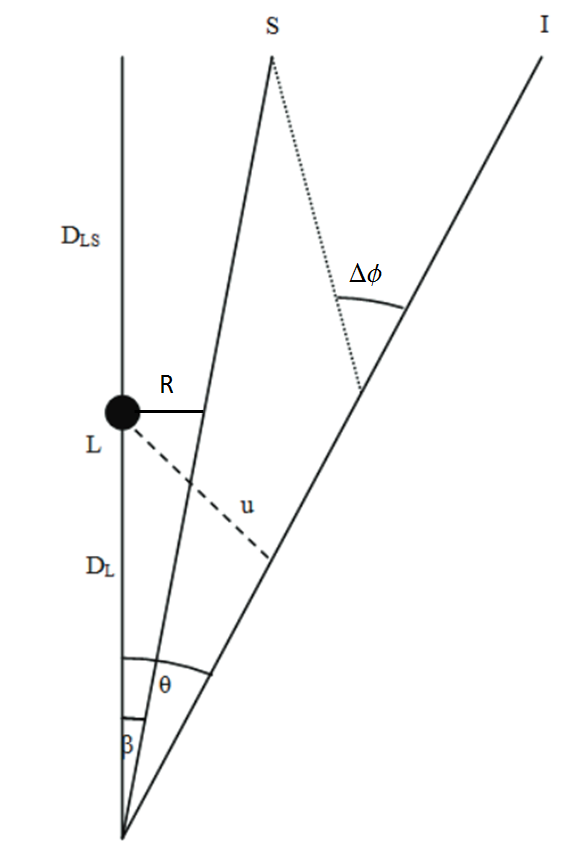
\includegraphics[scale=0.5]{LensEqFigure.png}
\captionof{figure}{A source emits light at position S.  The light is deflected by a massive lens at L, and causes the image seen by the observer to appear at an angle $\theta$.  D$_{LS}$, D$_L$, $\theta$, and $\beta$ are, respectively, the distance from the lens plane to the source plane, the distance from the lens plane to the observer, the angle of the image relative to the observer, and the angle of the source relative to the observer. \cite{Bin-Nun} }
\end{center}
 
Although there are only a few cases in which strong gravitational lensing can be observed, there are numerous cases of weak gravitational lensing.  Weak lensing occurs when the lensing mass isn't large enough for strong lensing, or if the source of light is not directly aligned with the lensing mass, resulting in a shear distortion of the image.  Measuring the mass of a weak lens is complicated by the fact that each light source has a unique, intrinsic ellipticity which typically dwarfs the magnitude of the image distortion.  This intrinsic ellipticity is known as ``shape noise" in weak gravitational lensing studies.  In cases where many sources are lensed by the same object, the distortion from the lens can be measured by averaging over the many source images, taking advantage of their random intrinsic orientation.  In these cases, the measured shear distortion results from photons being deflected by mass fluctuations along the line of sight.  In this case, the two dimensional lens equation (analogous to equation \ref{lens eq 2}) in vector format is
\begin{equation} \label{2D lens}
\boldsymbol{\beta} = \boldsymbol{\theta} - \frac{D_{LS}}{D_S} \Delta \boldsymbol{\phi}(\boldsymbol{\xi})
\end{equation}
where $\boldsymbol{\xi}=D_{S}\boldsymbol{\theta}$ is the impact parameter.  The deflection angle can be calculated by integrating the 3D gravitational potential, $\boldsymbol{\Phi}(\mathbf{r})$, along the line of sight such that
\begin{equation} \label{3D angle}
\Delta \boldsymbol{\phi}(\boldsymbol{\xi}) = 2 \int \nabla_\perp \boldsymbol{\Phi}(\mathbf{r})dz = \nabla_\perp(2\int \boldsymbol{\Phi}(\mathbf{r}) dz) \equiv \nabla_\perp V.
\end{equation}
Assuming the angle between the image and the observer, $\boldsymbol{\theta}$, is small equation \ref{2D lens} can be approximated with a first order Taylor series as
\begin{equation} \label{lens taylor}
\beta_{i}=A_{ij} \theta_{j}
\end{equation}
where $i$ corresponds to the $i^{th}$ component of the lens plane, $j$ corresponds to the $j^{th}$ component of the source plane, and 
\begin{equation} \label{dist matrix elements}
A_{ij}=\frac{ \partial \beta_i}{\partial \theta_j} = \delta_{ij} - \frac{ \partial \Delta \phi_i( \boldsymbol{\theta}) }{\partial \theta_j} = \delta_{ij} - 
\frac{ \partial ^2 V(\boldsymbol{\theta})} {\partial \theta_i \partial \theta_j}
\end{equation}
are the elements of a Jacobian distortion matrix, $\mathbf{A}$, which describes the isotropic dilation and anisotropic distortion due to convergence and shear effects.  The distortion matrix can be written in terms of the convergence, $\kappa$, which increases the size of the image while conserving brightness, and the shear, $\gamma$, which distorts the the image tangentially around the lens.  
\begin{equation} \label{dist mat}
A_{ij}=(1-\kappa)(\begin{matrix} 1 & 0 \\ 0 & 1 \end{matrix}) - \gamma(\begin{matrix} cos2\phi & sin2\phi \\ sin2\phi & -cos2\phi \end{matrix}) 
\end{equation}
Equations \ref{dist matrix elements} and \ref{dist mat} offer a relationship between the observable quantities $\kappa$ and $\gamma$, and the gravitational potential $V$.
\begin{equation} \label{gamma1}
\gamma_1 \equiv \gamma cos 2\phi= \frac{1}{2}[\frac{ \partial ^2 V(\boldsymbol{\theta})}{\partial \theta_1^2} - \frac{ \partial^2 V(\boldsymbol{\theta})}{\partial \theta_2^2}]
\end{equation}
\begin{equation} \label{gamma2}
\gamma_2 \equiv \gamma sin 2\phi = \frac{ \partial^2 V(\boldsymbol{\theta})}{\partial \theta_1 \partial \theta_2}
\end{equation}
\begin{equation} \label{kappa}
\kappa = \frac{1}{2} \nabla^2 V(\boldsymbol{\theta})
\end{equation}
where equation \ref{gamma1} comes from $A_{11}-A_{22}$, equation \ref{gamma2} comes from $A_{12}-A_{21}$, and equation \ref{kappa} comes from $tr(A)$.  Since $\kappa$ is equal to half the laplacian of the projected gravitational potential, $V$, it is directly proportional to the mass density of the lens.  The shear component $\gamma_1$ corresponds to elongation and compression along the $x$ and $y$ directions, and the component $\gamma_2$ describes elongation and compression along the diagonal $x=y$ and $x=-y$ directions.  In the case of weak lensing, the mass measurement then reduces to a measurement of the shear and convergence produced by the lens. \cite{Pires}. As with strong gravitational lensing, weak gravitational lensing mass measurements have been found to be consistent with dark matter models. \cite{Xiang}


\begin{center} \label{lensfigure}
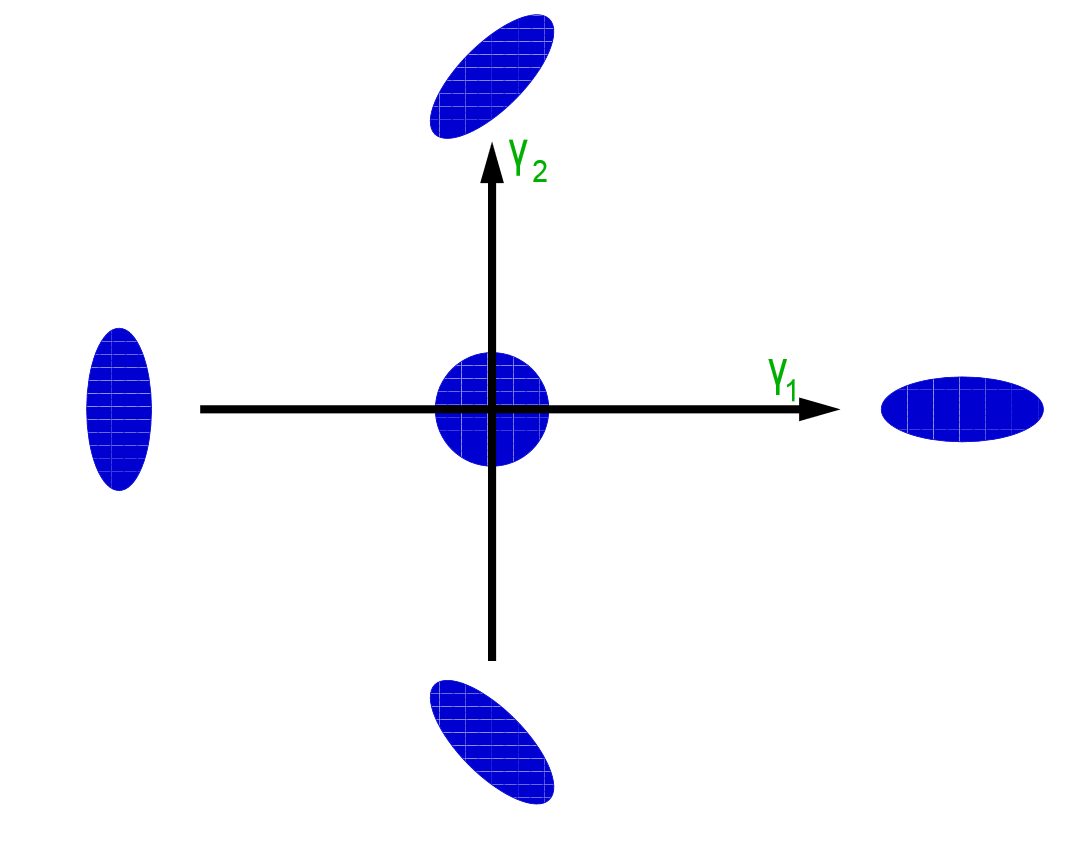
\includegraphics[scale=0.3]{GammaOneGammaTwo.png}
\captionof{figure}{An illustration of how positive and negative $\gamma_1$ and $\gamma_2$ distort an object with initial ellipticity of zero. \cite{Refregier} }
\end{center}

%trace of A equation
%\begin{equation}
%tr(\mathbf{A})=2-\frac{\partial^2V(\boldsymbol{\theta})}{\partial\theta^2_1} - \frac{\partial^2 V(\boldsymbol{\theta})}{\partial \theta^2_2} = 2-\nabla^2V(\boldsymbol{\theta})=2(1-\kappa)
%\end{equation}
 
One of the most famous instances of weak lensing evidence for dark matter is a collision of two galaxies clusters known as the Bullet Cluster.  The baryonic matter in each galaxy cluster is predominantly in the form of hot gas.  Electromagnetic interaction causes the gas to to slow down and concentrate in the center of the collision.  In the absence of dark matter gravitational lensing measurements should be correlated with the hot gas, since it is the dominant luminous mass in the system.  However, if dark matter was a dominant mass component in the Bullet Cluster it would not be slowed by electromagnetic interactions and would pass through the collision without significant perturbation. Indeed, weak gravitational lensing observations show that the majority of the mass in the Bullet Cluster passed through the collision rather than concentrating at the center like the luminous matter, suggesting that dark matter is present in abundance over the baryonic matter of the two galaxy clusters.  \cite{Clowe}


\begin{center} \label{bulletcluster}
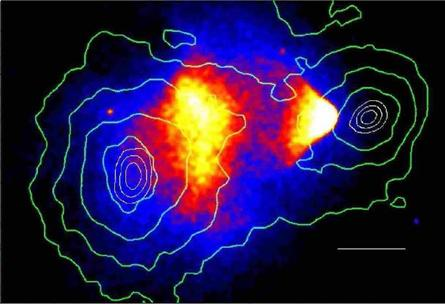
\includegraphics[scale=1]{bulletcluster.jpg}
\captionof{figure}{X-ray image of the baryonic mass in the Bullet cluster, overlayed with mass contours derived from weak lensing measurements.  The separation of the dominant mass component from the baryonic matter indicates the presence of dark matter.  \cite{Clowe} }
\end{center}
 

\subsubsection{Cosmological Evidence}

The early universe was filled with a hot, dense plasma of electrons and baryons.  At this time photons scattered off of the free electrons, restricting their movement across the universe.  As the universe cooled below the binding energy of hydrogen (13.6 eV) protons and electrons began to combine, forming neutral hydrogen atoms.  At this point in time, known as the recombination epoch,  photons and electrons decoupled and the photons began traveling with a mean free path the size of the universe.  These photons produce the Cosmic Microwave Background (CMB) that we see today. (Figure \ref{CMB_Planck})  The radiation is extremely isotropic and exhibits a black-body spectrum at a red shifted temperature of 2.72 K.  The frequency spectrum, temperature fluctuations, and polarization of the CMB all contain a vast amount of information about the formation of the universe.  Here, we focus on just one of these properties. 



\begin{center} \label{CMB_Planck}
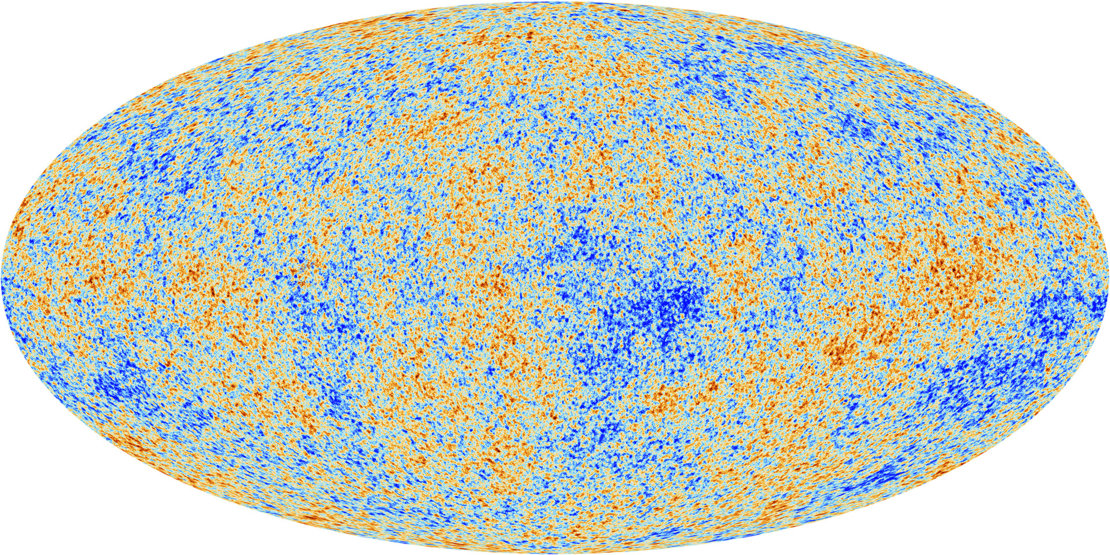
\includegraphics[scale=0.3]{CMB_Planck.jpg}
\captionof{figure}{The latest measurement of the CMB temperature anistropies from Planck data.  \cite{Planck} }
\end{center} 

In 2003 the WMAP satellite observed small (1 part in 10,000) fluctuations in the average temperature of the CMB.  We see these temperature fluctuations projected on a 2D spherical surface, so it is typical to expand them in terms of spherical harmonics defined by
\begin{equation}\label{Ylm}
Y_{lm}=\sqrt{\frac{2l+1}{4\pi} \frac{(l-m)!}{(l+m)!}}P_l^m(cos\theta)e^{im\phi}
\end{equation}
where $l=0,...,\infty$, $-l \le m \le l$, and $P_l^m$ are associated Legendre polynomials.  The temperature fluctuations can then be written as
\begin{equation}\label{dTdT0}
f(\theta,\phi) \equiv \frac{\delta T(\theta,\phi)}{T_0} = \sum_{l=0}^{l=\infty} \sum_{m=-l}^{m=l} a_{lm} Y_{lm}(\theta,\phi)
\end{equation}
where $T_0$ is the average temperature of the CMB and $a_{lm}$ are the coefficients of expansion. Since the spherical harmonics are orthonormal
\begin{equation}\label{alm}
a_{lm} = \int_{\theta=-\pi}^{\pi}\int_{\phi=0}^{2\pi} f(\theta,\phi)Y_{lm}^*(\theta,\phi) d\Omega
\end{equation}
and since $a_{lm}$ are independent random variables
\begin{equation}\label{alm_var1}
\mean{a_{lm}a_{l'm'}^*} = \delta_{ll'}\delta{mm'}\mean{|a_{lm}|^2}.
\end{equation}
The temperature fluctuations are isotropic and therefore independent of m, so
\begin{equation}\label{alm_var2}
\mean{|a_{lm}|^2}=\frac{1}{2l+1} \sum_{m}\mean{|a_{lm}^2|} \equiv C_l.
\end{equation}
where the function $C_l$ is referred to as the angular power spectrum of the temperature fluctuations.  The angular power spectrum is related to contribution of the multipole $l$ to the temperature variance by
\begin{align}\label{powerspec}
\mean{\left(\frac{\delta T(\theta,\phi)}{T_0} \right)^2} \begin{aligned} = \end{aligned} \mean{\sum_{lm}a_{lm}Y_{lm}(\theta,\phi)\sum_{l'm'}a_{l'm'}^*Y_{l'm'}^*(\theta,\phi)} \nonumber \\
\begin{aligned} = \end{aligned} \sum_{ll'}\sum_{mm'}Y_{lm}(\theta,\phi)Y_{l'm'}^*(\theta,\phi)\mean{a_{lm}a_{l'm'}^* } \\
\begin{aligned} = \end{aligned} \sum_l C_l \sum_m |Y_{lm}(\theta,\phi)|^2 = \sum_l \frac{2l+1}{4\pi}C_l  \nonumber
\end{align}
where we have used the the closure relation
\begin{equation}\label{closure}
\sum_m |Y_{lm}(\theta,\phi)|^2 = \frac{2l+1}{4\pi}
\end{equation}
in the last step of equation \ref{powerspec}. \cite{Kurki-Suonio}


Cosmological models predict the variance of the $a_{lm}$ expansion coefficients, and therefore predict the angular power spectrum and the contribution of each multipole to the temperature variance.  By measuring the angular power spectrum of the CMB and comparing to the $C_l$ values predicted by each model we can learn about the composition of the universe.  The temperature fluctuations of the CMB are typically plotted as $l(l+1)C_l/(2\pi)$ with units of $\mu K^2$ versus the multipoles $l$ as shown in Figure \ref{PS_Planck}.

\begin{center} \label{PS_Planck}
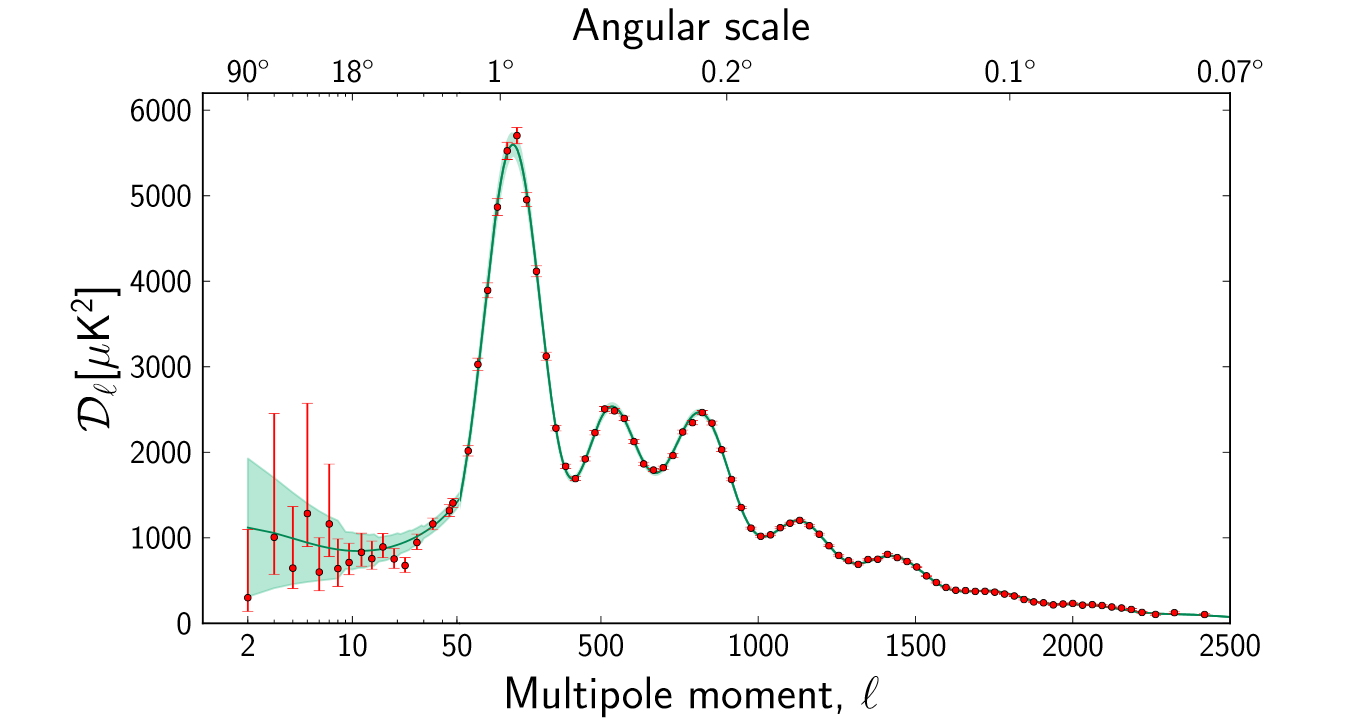
\includegraphics[scale=0.4]{PS_Planck.png}
\captionof{figure}{The power spectrum of temperature fluctuations from the CMB based on data from Planck. \cite{Planck} }
\end{center} 


To understand the wealth of information present in Figure \ref{PS_Planck} we must first understand the origin of the temperature fluctuations in the early universe.  Prior to recombination the primordial plasma consisted of anistropic regions of varying density. Overdense regions of matter would gravitationally attract more matter.  As this happened, heat from photons scattering off of free electrons would produce an increase in pressure, counteracting the force of gravity and pushing baryonic matter away from the high density regions.  As these two processes competed they produced oscillations in the distribution of baryonic matter, which we refer to as Baryon acoustic oscillations (BAO).  After recombination the photons diffused through the baryonic matter, removing the source of pressure, ending the oscillating process, and leaving a shell of overdense baryonic matter at the origin of the anisotropy and at a fixed radius called the sound horizon.

The first peak in Figure \ref{PS_Planck} details the curvature of the universe. If the universe had positive curvature the light from the CMB would be magnified, shifting the first peak to lower multipole in Figure \ref{PS_Planck}.  Likewise, in a negatively curved universe the scale of the temperature fluctuations in the CMB would appear diminished, shifting the first peak to higher multipole.  The observed location of the first peak, close to $l\sim$200, turns out to be consistent with a flat universe.  

The second peak in Figure \ref{PS_Planck} details the amount of baryonic matter in the universe.  Baryons add mass to the system during the oscillating process described above.  This additonal inertia forces the primordial plasma to travel farther before recoiling back to the center of the anistropy, much like adding a mass to the end of a spring.  The odd numbered peaks in Figure \ref{CMB_Planck} are associated with how far the plasma compresses during BAO and are enhanced by the presence of additional baryons, as shown in Figure \ref{BAO}.  The even numbered peaks are associated with how far the plasma rebounds during BAO and are unaffected by the presence of additional baryons.  Therefore, the presence of baryons enhances the size of the odd peaks over the even peaks such that a smaller second peak in Figure \ref{PS_Planck} corresponds to a larger amount of baryonic matter in the universe.  The latest results from Planck indicate that baryonic matter makes up 4.9\% of the universe.


\begin{center} \label{BAO}
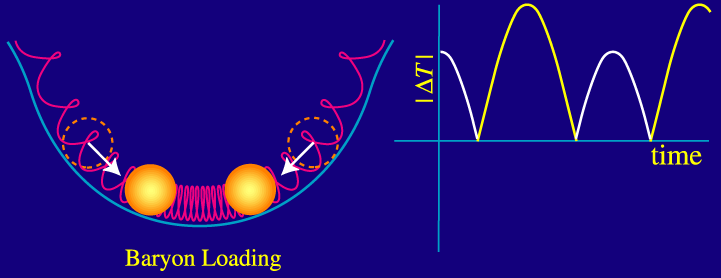
\includegraphics[scale=0.7]{BAO.png}
\captionof{figure}{A depiction of the effect of baryons on the oscillating plasma during BAO.  The mass of the baryons loads down the plasma, producing an asymmetry in the oscillations in which the plasma compresses further toward the minimum of the potential well. Since the CMB power spectrum does not care about the sign of the fluctuation, we see that the odd numbered peaks become enhanced over the even numbered peaks.  \cite{Whu} }
\end{center} 

The third peak in Figure \ref{PS_Planck} details the amount of dark matter in the universe.  Since the very early universe was dominated by photon-baryon interactions, the outward pressure caused the gravitational potential of the BAO system to decay in such a way that it drove the amplitude of oscillations higher.  With higher dark matter density this driving effect is diminished and the overall magnitude of the peaks becomes smaller.  Although this effects all of the peaks in Figure \ref{PS_Planck} it is only distinguishable in the third peak.  Furthermore, as with ordinary matter, dark matter was gravitational attracted to areas with higher density.  Since dark matter does not interact through the electromagnetic force it was unaffected by the increasing photon pressure which produced acoustic oscillations in baryons.  As a result, a higher density of dark matter corresponded to a larger gravitational potential well for baryons to fall into during their oscillations, increasing the amplification of BAO on the odd numbered peaks.  Therefore, the height of the third peak tells us the amount of dark matter that is present in the universe. \cite{Whu} The Planck observations indicates that dark matter makes up 26.8\% of the universe.  The remaining 68.3\% of the universe is made up of dark energy. \cite{Planck}


%INCLUDE COBE MAP AND COBE POWER SPECTRUM

%This should be in the next chapter -- Dark Matter Candidates
\subsection{Dark Matter Candidates}

\subsubsection{The $\Lambda$CDM Model}
To further examine the properties of dark matter it is useful to introduce a quantitative measure for the composition of the universe.  Friedmann's equation, which describes the expansion of space in a homogeneous and isotropic universe, is given by
\begin{equation}\label{Friedmann's}
\frac{\dot{a}^2 + kc^2}{a^2} = \frac{8 \pi G \rho + \Lambda c^2}{3},
\end{equation}
where $a$ is the scale factor of the universe, $k$ is the spatial curvature of the universe (equivalent to one sixth of the Ricci Scalar) , $c$ is the speed of light, $G$ is the gravitational constant, $\rho$ is the density of the universe, and $\Lambda$ is the cosmological constant. Einstein's field equations,
\begin{equation}\label{EFQ}
G_{\mu\nu} = \frac{8 \pi G}{c^4} T_{\mu\nu}
\end{equation}
provide an expression for the cosmological constant, $\Lambda$.  We can split the stress energy tensor into two terms, one describing matter and the other describing the vacuum, such that $T_{\mu\nu}=T_{\mu\nu}^{matter}+T_{\mu\nu}^{vac}$.  Since the stress energy tensor is given by
\begin{equation}\label{StressTensor}
T_{\mu\nu} = (\rho + p)U_{\mu}U_{\nu} + pg_{\mu\nu},
\end{equation}
and to maintain Lorentz invariance $p^{vac} = -\rho^{vac}$, we can write the vacuum component of the stress energy tensor as
\begin{equation}\label{StressTensorVac}
T_{\mu\nu}^{vac}=-\rho^{vac} g_{\mu\nu}.
\end{equation}
If we identify the vacuum energy density as
\begin{equation} \label{VacEnergyDens}
\rho^{vac}=\frac{\Lambda c^2}{8\pi G}
\end{equation}
then Einstein's field equation takes on the familiar form
\begin{equation}\label{EFQ2}
G_{\mu\nu} + g_{\mu\nu}\Lambda= \frac{8 \pi G}{c^4} T_{\mu\nu}^{matter},
\end{equation}
where $G_{\mu\nu}$ is the Einstein tensor, $g_{\mu\nu}$ is the metric tensor, $G$ is the gravitational constant, and $\Lambda$ is the cosmological constant.
Setting the normalized spatial curvature $k = 0$ in Friedmann's equation(representing a flat universe), one can find the critical density for which the universe is spatially flat to be
\begin{equation}\label{RhoC}
\rho_c = \frac{3}{8 \pi G}\frac{\dot{a}^2}{a^2},
\end{equation}
where $\rho_c = \rho^{vac}+\rho$.
Recognizing Hubble's constant to be $ H = \frac { \dot{a}}{a} $, we can rewrite this as
\begin{equation}\label{RhoC2}
\rho_c =\frac{3H^2}{8 \pi G}
\end{equation}
where $H$ is the present value of the Hubble constant \cite{Javorsek}. The current experimental value for $H$ in the dimensionless units 100 km/s/Mpc is $ h \sim 0.7 $ with an uncertainty of $\sim5\%$.  We can then define the density parameter as 
\begin{equation} \label{Omega}
\Omega=\frac{\rho}{\rho_c}=\frac{8 \pi G \rho}{3 H_0^2}.
\end{equation}
If $\Omega$ is larger than unity the universe is spatially closed, and if $\Omega$ is less than unity the universe is spatially open. This density parameter can be split into components, such that for a particular component $x$
\begin{equation} \label{OmegaComp}
\Omega_x = \frac{\rho_x}{\rho_c}.
\end{equation}

Detailed cosmological studies have concluded that all the luminous matter in the universe has a density parameter of $\Omega_{lum} \lesssim 0.01$.  This information, combined  with the fact that analysis of galactic rotational velocities implies $> $90\% of the mass in galaxies is dark leads to the conclusion that $\Omega_{DM} \geq 0.09$.  This is only a lower limit on the dark matter density parameter, since most rotation curves remain flat out to the largest radii at which they can be measured and it can be assumed that the DM halos extend even further out.


With $\Omega_{DM} \geq 0.1$ it is possible that baryonic DM alone could be responsible for the dark matter halos.  However, other analyses eliminate this possibility. Direct searches for massive compact halo objects (MACHOs) utilizing microlensing have determined that $<$25\% of the dark halos could be due to baryonic dark matter within the mass range of $ 2 \times 10^{-7} M_{sun} < M < 1 M_{sun} $ at a 95\% confidence limit \cite{EROS,Alcock}. Furthermore, data from the Hubble Deep Field Space Telescope suggests dark matter halos consist of $\leq$5\% white dwarfs.

With baryonic dark matter being ruled out as the sole component of dark matter halos we now investigate the other density parameter components. Big Bang nucleosynthesis models constrain the amount of baryonic matter in the universe to $\Omega_b \approx 0.045$ (where b stands for baryons) \cite{Tytler}.  Additionally, analysis of velocity flows, x-ray emissions temperatures, and gravitational lensing in large clusters and superclusters of galaxies suggests that the total matter component of the universe has density parameter $\Omega_m \approx 0.2-0.3$.  One can combine this information, assuming $h=0.7$ to find that
\[\Omega_b = 4.9\% \]
\[\Omega_{nbm} = 26.8\% \]
\[\Omega_\Lambda = 68.3\%\]
where $\Omega_b$ is the baryonic density of the universe, $\Omega_{nbm}$ is the nonbaryonic density parameter of the universe, and $\Omega_\Lambda$ is the dark energy density parameter of the universe \cite{Spergel,Planck}. This is known as the $\Lambda$-CDM model. 

\subsubsection{Nonbaryonic Dark Matter}

With $\Omega_{nbm} = 26.8\% $ it is intriguing to look at the particles which have been proposed to explain this contribution to the total density parameter. One such particle is the standard-model neutrino.  The neutrino is an electrically neutral, weakly interacting particle with a nearly zero mass.  Neutrinos exist in three distinct flavors -- the electron neutrino ($\nu_e$), the muon neutrino ($\nu_\mu$), and the tau neutrino ($\nu_\tau$).  It is known that neutrinos oscillate between these three flavors, with each flavor state being a super position of three neutrino states of definite mass ($\nu_1$,$\nu_2$, and $\nu_3$).  Experiments studying solar neutrino oscillations have determined the squared mass difference between what is known as the solar neutrino doublet ($\nu_1$ and $\nu_2$) to be $\delta m^2 = (7.66 \pm 0.35) \times 10^{-5} eV^2$, while experiments studying atmospheric neutrino oscillations have determined the remaining squared mass difference between the solar neutrino doublet and $\nu_3$ to be $\pm (2.38 \pm 0.27) \times 10^{-3} eV^2$ up to an unknown sign \cite{Robertson}.  This sign ambiguity leads to two possible hierarchies for the neutrino mass states. (Figure \ref{neutrinos})  If we assume the normal hierarchy to be true, we can set a lower limit on the most massive neutrino state to be $ m_{\nu_3} \gtrsim 0.05$ eV.

\begin{center}
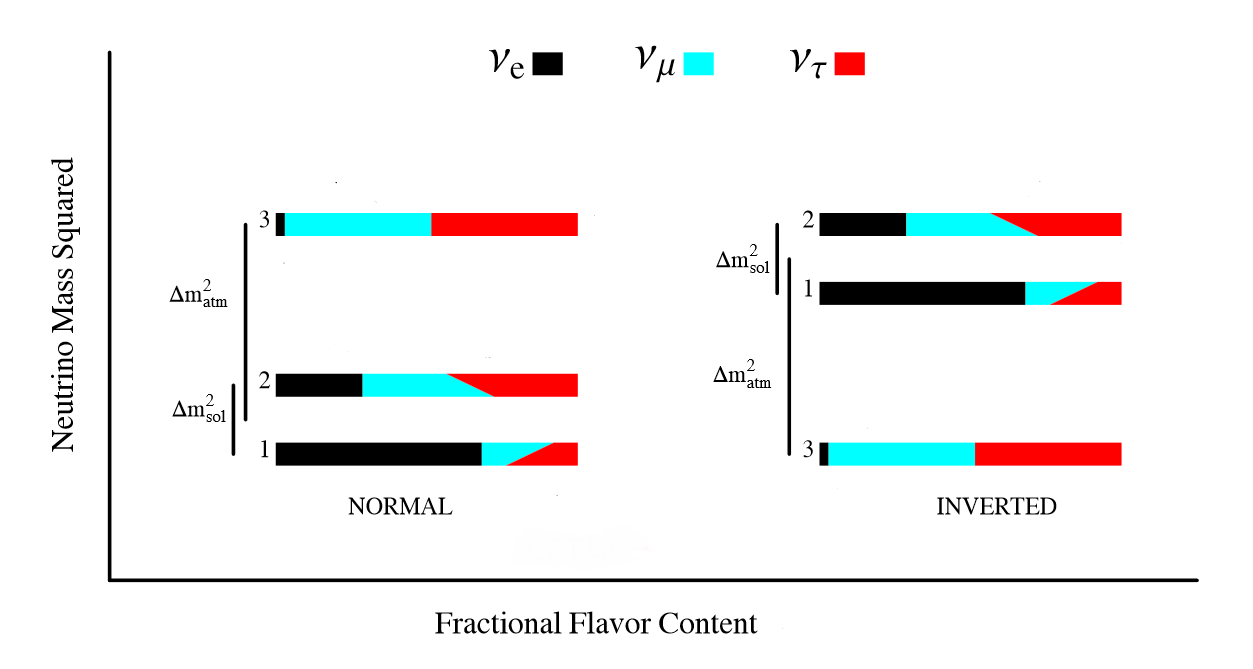
\includegraphics[scale=0.4]{neutrinos.png} \label{neutrinos}
\captionof{figure}{The two hierarchies of neutrino mass states.  Black, teal, and red indicated the three flavors of neutrinos, while one, two, and three indicated the three mass states. Reproduced from Reference \cite{Parke}.}
\end{center}


The density parameter of neutrinos is given by
\[\Omega_\nu=\frac{\rho_\nu}{\rho_c}=\frac{1}{h^2}\sum_{i=1}^3 \frac{g_i m_i}{90eV},\]
where $g_i = 1$ for Majorana neutrinos (own antiparticle) and $g_i = 2$ for Dirac neutrinos (distinct antiparticles) \cite{Pastor}. Using the lower mass limit of the neutrino and assuming Majorana neutrinos, this suggests a lower limit on the neutrino density parameter of $\Omega_\nu \gtrsim 0.00122$.  Thus, neutrinos do provide some contribution to the nonbaryonic dark matter density parameter.  

To find an upper limit on the neutrino contribution to the nonbaryonic dark matter density parameter is is necessary to distinguish hot dark matter from cold dark matter.  Hot dark matter is composed of particles that have zero or nearly-zero mass.  Special relativity requires that the massless particles move at the speed of light, and that the nearly-massless particles move close to the speed of light.  As a result hot dark matter forms very hot gases.  Cold dark matter is composed of particles that have sufficient mass to travel at sub-relativistic velocities, thus forming colder gases.  With their low masses neutrinos fall under the hot dark matter category.  A combination of galaxy clustering measurements, CMB observations, and Lyman-$\alpha$ observations give an upper limit on the hot dark matter contribution of $\Omega_\nu \lesssim 0.0155$, thus neutrinos and other hot dark matter particles cannot be the primary contribution to the nonbaryonic dark matter density parameter \cite{Spergel}.

\subsubsection{WIMPs and SUSY} \label{WIMPSandSUSY}

If we assume cold dark matter (CDM) particles were in thermal equilibrium with the other standard-model particles during the early stages ($<$1 ns) of the universe it is possible to calculate the CDM density parameter.  According to Maxwell-Boltzmann statistics, as the temperature, $T$, of the universe cools, the particles with masses $m > T$ will diminish exponentially.  Once the temperature of the universe cooled below the CDM mass scale the creation of these particles would have ceased.  At this time the CDM particles which still existed would have continued annihilating with one another.  As time went on, CDM annihilation became less and less likely due to their dwindling abundance.  Once the expansion rate of the universe, given by Hubble's constant, exceeded the CDM annihilation/creation rate, the CDM particles dropped out of thermal equilibrium and the CDM density became fixed.  

The density parameter for CDM is approximately given by
\[\Omega_\chi h^2 \simeq \frac{T_0^3}{M_{Pl} \langle \sigma_A \nu \rangle} \]
where $\sigma_A$ is the total annihilation cross section of CDM particles, $\nu$ is the relative velocity of CDM particles, $T_0$ is the equilibrium temperature, $M_{Pl}$ is the Planck mass, $c$ is the speed of light, and $\langle ... \rangle$ represents an average over the thermal distribution of CDM particle velocities \cite{Kolb,Jungman}. Remarkably, for the total density parameter of the universe to equal unity, as required by cosmological models, a cross section on the order of particles interacting on the electroweak scale ($\sim 10^{-9} GeV^{-2}$) is required for CDM particles. This result is the main motivation behind suspecting weakly interacting massive particles (WIMPs) as the dominant contribution to the nonbaryonic dark matter density parameter.  

Supersymmetry (SUSY) is a symmetry of space-time which has been proposed in an effort to unify the electroweak, strong, and gravitional forces.  This theory offers some insight into the nature of WIMPs.  SUSY requires that a supersymmetric partner particle exists for each particle in the standard model.  These partners go by the names of sleptons (partners of leptons), squarks (partners of quarks), gauginos (partners of gauge bosons), and higgsinos (partners of Higgs bosons).  Sleptons and squarks have spin zero, while gauginos and higgsinos have spin one-half.  Since none of these supersymmetric particles have been discovered it is thought they are far more massive than their standard model counterparts, and thus that supersymmetry is not an explicit symmetry of nature.
  
Goldberg \cite{Goldberg} and Ellis \cite{Ellis} have suggested that neutral gauginos and neutral higgsinos can mix together in a superposition known as the neutralino, $\chi$.  In most SUSY models, the neutralino is the lightest supersymmetric particle (LSP).  In models which conserve R-parity (a new quantum number distinguishing SUSY particles from standard model particles) the LSP is stable, making it a prime candidate particle for dark matter.  The expected cross section of neutralinos interacting via inelastic collisions with nucleons is dependent on the allowed regions of parameter space in the SUSY model being used.  Results from the WMAP satellite refined this parameter space, concluding that the density parameter of neutralinos would be  $0.192 < \Omega_\chi < 0.263$ \cite{Spergel,Bennett,Arnowitt}.

The neutralino is one of many candidate particles suggested for WIMPs, and as previously mentioned, WIMPs are not the only candidate for dark matter.  In the following sections we will briefly discuss some of the other candidates before returning to the discussion of WIMPs in Chapter \ref{Chapter2}.

\subsubsection{Axions and Axinos}
Quantum chromodynamics (QCD) is a theory describing the strong interaction between quarks and gluons, which make up hadrons.  In particle physics there exists a proposed symmetry of nature referred to as charge conjugation parity symmetry (CP-Symmetry).  CP-Symmetry postulates that particles should behave the same if they are replace by their own antiparticle (C symmetry), and then have their parity reversed (P symmetry). Within QCD there is no theoretical reason to assume CP-symmetry exists.  However, when a CP-violation term is included in the QCD lagrangian its coefficient has been experimentally determined to be less than $10^{-10}$ \cite{Baluni}. This unexpected result is known as the strong CP problem in quantum chromodynamics.    To reconcile this, a new symmetry known as the Peccei-Quinn theory has been proposed.  This theory postulates the existence of a new pseudoscalar particle called the axion.  According to the Peccei-Quinn theory, axions would be electrically neutral, low mass ( $1\mu eV - 1 eV$) particles that have very low interaction cross sections for the strong and weak forces.  The axino arises when SUSY is introduced to the Peccei-Quinn theory, resulting in a supersymmetric partner to the axion known as the axino.

\subsubsection{Gravitons and Gravitinos}
In quantum field theory, the graviton is a hypothetical  elementary particle which mediates the gravitational force.  As with axions and axinos, when SUSY is introduced to quantum field theory a supersymmetric partner to the graviton is predicted to exist known as the gravitino.  In some models, gravitinos are the LSP in SUSY and are thus a candidate particle for dark matter.

\subsubsection{WIMPzillas}
WIMPzillas are supermassive dark matter particles which arise when one considers the possibility that dark matter might be composed of nonthermal supermassive states. These particles would have a mass many orders of magnitude higher than the weak scale \cite{Chung}. Studies have shown that for stable particles with masses close to $10^{13} \; GeV$  WIMPzillas would be produced in sufficient abundance to give $\Omega \approx 1$ for the total density parameter of the universe.  

It should be noted that the discussion of this section does not encompass all of the alternatives to WIMPs.   Although these other dark matter candidates offer intriguing explanations to the dark matter problem, the next chapter will focus on the experimental detection of WIMPs.

%http://arxiv.org/pdf/hep-ph/0404175v2.pdf was used as a heavy resource here.. not sure where to cite it though
\section{Searching for WIMPs} \label{Chapter2}

The search for WIMPs can be separated in three categories: indirect detection, direction detection, and WIMP creation. \cite{Bertone}  Direct detection experiments search for the scattering of dark matter particles off of atomic nuclei and will be the topic of this thesis from Chapter 3 onward. Indirect detection experiments search for remnants of WIMP interactions such as gamma-rays, positrons, and neutrinos using both space based and ground based detectors.  Similarly, high energy particle colliders are used to search for missing energy signals during WIMP that may be produced during their collisions.

\subsection{Indirect Detection Experiments}

In section \ref{WIMPSandSUSY} we discussed the annihilation of CDM particles such as WIMPs during the early universe.  WIMP annihilation can produce gamma-rays, neutrinos, and positrons.  Numerous indirect detection experiments search for these annihilation remnants in gravitational wells where the dark matter density is expected to be high, such a the center of the Sun.  In the following sections, we will discuss efforts to detect each annihilation product separately.

\subsubsection{Gamma-Ray Experiments}

WIMP annihilation is expected to produce monoenergetic photons with an energy given by
\begin{equation} \label{WIMP-penergy}
E_{\gamma} = m_{\chi} (1-\frac{m_X^2}{4m_\chi^2})
\end{equation}
where $m_\chi$ is the mass of the WIMP and $m_X$ is the mass of the remnant particle.  At the GeV energy scale photons interact with matter via electron-positron pair production, leading to an interaction length much shorter than the thickness of Earth's atmosphere.  As a result, any experiment seeking to directly detect gamma-ray radiation from WIMP annihilation must be based in space.  Satellites such as the Fermi-LAT detect the electron-positron pairs produced by gamma-ray interaction in a detector made of a dense material (in the case of Fermi-LAT, tungsten is used).  These space based detectors are hindered by the numerous sources of background radiation present in astrophysical data, and are therefore unable to make significant claim of detection without observing a monoenergetic signal across multiple sources.  As of 2012 the Fermi-LAT has observed no such line features or significant gamma-ray flux in its data. \cite{Fermi-LAT} 

When gamma-rays interact with the atmosphere they produce an cascade of secondary particles.  These seconday particles produce Cerenkov radiation as they pass through the atmosphere, allowing ground-based telescopes to search for the gamma-ray product of WIMP annihilation indirectly.  Cosmic ray radiation can also induce Cerenkov radiation in the atmosphere, making the it difficult to distinguish gamma-ray sources from the cosmic ray background.  Ground based experiments employ numerical simulations of atmospheric showers and require an excess of directional gamma-rays above the isotropic background induced by cosmic rays to overcome this challenge. \cite{Knapp}  As with space based experiments, ground based experiments have yet to observe a gamma-ray flux above background in their data. \cite{HESS, VERITAS}

\subsubsection{Neutrino Experiments}

Neutrinos from WIMP annihilation can interact with ordinary matter via a charge current interaction or a neutral current interaction.  In a charged current interaction, a high energy neutrino transforms into its lepton partner via a process such as inverse beta decay ($\bar{\nu_e} + p \rightarrow n + e^+ $).  These neutrino interactions are ideal to work with, since the leptons are easy to detect and allow the neutrino to be flavor-tagged.  However, if a neutrino has less energy than the mass of its lepton partner it can not interact via a charge current interaction.  In a neutral current interaction the neutrino remains as a neutrino but deposits energy and momentum onto a target particle.  If the target is light, such as an electron, it can be accelerated above the speed of light in the medium and produce Cerenkov radiation.  

Ground based detectors, such as ANTARES and IceCube, search for the neutrinos produced in dark matter annihilation by observing the Cerenkov radiation from muon tracks produced in charged current interactions at the GeV-TeV energy scale.  These detectors utilize large photo-multiplier arrays buried deep in a transparent medium, such as the antartic ice, to avoid background from cosmic rays.  These experiments have not observed any dark matter annihilation signal from dark matter particles at the center of the Sun or in nearby galaxy clusters, but have set the world's best spin-dependent cross section limits for WIMPs in the process. \cite{IceCube, IceCube2}

\subsubsection{Positron Experiments}

Positrons can be produced with a varying spectrum via direct annihilation of dark matter to positron-electron pairs or by annihilations to ZZ or W$^+$W$^-$.  \cite{Cheng,Kamionkowsk}.  These positrons do not travel in straight lines from their source due to galactic magnetic fields.  Due to their low mass, electrons and positrons lose energy via inverse Compton scattering and synchrotron radiation as they travel from source to observer. The energy loss increases with the square of the electron energy, such that the power law energy spectrum is steepened at the location of the observer, resulting in an expectation of $\sim E^-3$.  The inelastic collision of cosmic-ray protons and $\alpha$-particles produce charged pions, which in turn produce secondary positrons and electrons in roughly equal amounts via the $\pi-\mu-e$ decay chain. \cite{Stecker}  For secondary electrons and positrons, the source spectrum would therefore follow the energy spectrum of ambient protons, which is approximately $\sim E^-3.7$ after radiative loss during transit.  If the only source of positrons was from secondary production, and astrophysical sources produced electron, we would then expect the positron fraction $e^+/(e^+ + e^-)$) to decrease smoothly with energy.  \cite{PEBS} Therefore, experiments which seek to measure a positron signal from dark matter annihilation observe the positron fraction as a function of energy from entire galactic halo and compare their results to astrophysical models of positron production.

Experiments such as FERMI-LAT, PAMELA, and AMS-02 have confirmed a rise in the positron fraction at high energy. \cite{FermiPositron,PamelaPositron,AMSPositron} However, a very high cross section and leptophilic models are required for these observations to be attributed to dark matter annihilation.  Alternative explanations such as local pulsar sources and acceleration of secondary positrons have also been proposed. \cite{Serpico}



\subsection{WIMP creation in Colliders}

Experiments such as ATLAS and CMS are using the Large Hadron Collider (LHC) beneath France and Switzerland to search for the production of WIMPs in high energy particle collisions.  The LHC is a proton-proton collider which should have a large production cross section for colored super symmetric particles.  The WIMP pair production interaction $pp (p\bar{p}) \rightarrow \chi \bar{\chi}$ is of no use in these experiments, since it leaves no observable signal in the detector.  Instead, these experiments try to observe the higher order $pp (p\bar{p}) \rightarrow \chi \bar{\chi} + jets$ interaction, with the jets serving as a trigger that an event took place.  The dominant background when looking for such an event comes from the electroweak processes where the Z decays into a pair of neutrinos $pp (p\bar{p}) \rightarrow \nu \bar{\nu} + jets$ or the $W^{\pm}$ decays into a neutrino and a lepton $pp (p\bar{p}) \rightarrow l^{-}\bar{\nu} + jets$ or $pp (p\bar{p}) \rightarrow l^{+}\nu + jets$. In a WIMP $+$ jets event the WIMP will exit the detector unseen, producing a signature with missing transverse momentum.  The magnitude of this missing momentum is typically denoted as $E_T^{miss}$.  A model independent approach shows that $E_T^{miss}$ should be detectable at the LHC under the assumption that all new particles mediating the interaction of WIMPs and standard model particles are too heavy to be produced directly.  \cite{Beltran} However, no excess of events beyond the standard model processes has been observed at the LHC as of yet.  \cite{ATLAS}


\subsection{Direct Detection Experiments}
If dark matter interacts through the weak force, then it should be possible to observe WIMPs via nuclear recoils in direct detection experiments. During these events, a WIMP will scatter off of a target nucleus in the detector, producing a signal in the range of 1-100 keV. \cite{Lewin}   Direct detection experiments typically observe ionization, scintillation, or low temperature phonons produced during the event (or a combination of the three), although more recent experiments have developed an acoustic method of detection based on producing bubbles in a superheated fluid at the cite of a recoil.  These signals are susceptible to both nuclear recoil and electron recoil backgrounds so detailed, in situ, calibrations are required to characterize the detector's response to each type of event.  In this section, we will first review the WIMP recoil spectrum before discussing the different types of direct detection experiments in detail.  In the following chapter we will describe the one particular experiment, the LUX detector, in great detail before reviewing standard calibration techniques in chapter \ref{StandardCalibrations}.

\subsubsection{The WIMP Recoil Spectrum}

Lewin and Smith provide a standard derivation of the expected WIMP recoil spectrum in reference \cite{Lewin}.  Their derivation begins with the differential particle density is given by 
\begin{equation}
dn=\frac{n_0}{k} f(\mathbf{v},\mathbf{v_E}) d^3\mathbf{v}
\end{equation}
where $n_0$ is the mean dark matter particle density, $\mathbf{v}$ is the velocity of the WIMP relative to the target, $\mathbf{v_E}$ is the velocity of the earth relative to the WIMP, $f(\mathbf{v},\mathbf{v_E})$ is the WIMP velocity distribution function.  The normalization constant $k$ is given by
\begin{equation}
k=\int_0^{2\pi}\int_{-1}^{1} \int_0^{v_{esc}}  f(\mathbf{v},\mathbf{v_E}) v^2 d(cos\theta)dv
\end{equation}
where $v_{esc}$ is the local escape velocity, so that 
\begin{equation}
\int_0^{v_esc}dn \equiv n_0.
\end{equation}
We treat the dark matter as a non-interacting ideal gas so that we can assume a Maxwellian dark matter velocity distribution given by
\begin{equation}
f(\mathbf{v},\mathbf{v_E})=e^{(-v+v_{E})^2/v_0^2}.
\end{equation}
Then for $v_{esc}=\infty$ we define
\begin{equation} \label{k-not}
k_0 \equiv (\pi v_0^2)^{3/2},
\end{equation}
and for finite escape velocity $v_{esc}=|\mathbf{v}+\mathbf{v_E}|$,
\begin{equation}
k=k_0[\mbox{erf}(\frac{v_{esc}}{v_0}) - \frac{2}{\sqrt{\pi}} \frac{v_{esc}}{v_0} e^{-v_{esc}^2/v_0^2}].
\end{equation}

The event rate per unit mass on a target of atomic mass $A$ (AMU), with cross-section per nucleus $\sigma$ is given by
\begin{equation}
dR=\frac{N_0}{A} \sigma v dn
\end{equation}
where $N_0$ is Avogadro's number ($6.02\times10^{26} mol^{-1}$).  For constant cross section $\sigma=\sigma_0$ the even rate per unit mass is then
\begin{equation}
R=\frac{N_0}{A}\sigma_0 \int v dn \equiv \frac{N_0}{A}\sigma_0n_0\left\langle v\right\rangle .
\end{equation}
Substituting $n_0=\rho_{\chi} / M_{\chi}$ (where $\rho_{\chi}$ and $M_{\chi}$ are the WIMP density and mass, respectively) we define the event rate per unit mass for $v_E=0$ and $v_{esc}=\infty$ as
\begin{equation} \label{R-not}
R_0=\frac{2 N_0 \rho_{\chi}}{\sqrt{\pi} A M_{\chi}} \sigma_0 v_0 = \frac{2 \rho_{\chi} }{\sqrt{\pi} M_{\chi} M_T} \sigma_0 v_0
\end{equation}
where $M_T$ is the mass of the WIMP, such that 
\begin{equation} \label{intR}
R=R_0 \frac{\sqrt{\pi} \left \langle v \right \rangle}{2 v_0} = R_0 \frac{k_0}{2 \pi v_0^4 k} \int v f(\mathbf{v},\mathbf{v_E}) d^3v.
\end{equation}
In differential form equation \ref{intR} becomes
\begin{equation} \label{diffR}
dR = R_0 \frac{k_0}{2 \pi v_0^4 k} v f(\mathbf{v},\mathbf{v_E}) d^3v.
\end{equation}

The recoil energy (as measured in the lab frame) of a nucleus struck by a WIMP of kinetic energy $E=\frac{1}{2} M_\chi v^2$ and scattered at an angle $\theta$ in a center-of-mass frame if given by
\begin{equation}
E_R= \frac{1}{2} M_\chi v^2 \frac{2 M_\chi M_T}{(M_\chi + M_T)^2} (1-cos\theta).
\end{equation}
For isotropic scattering recoils are uniformly distributed over a range of $0 \leq E_R \leq \frac{1}{2} M_\chi v^2 \frac{4 M_\chi M_T}{(M\chi + M_T)^2}$ so
\begin{equation} \label{dRdER}
\frac{dR}{dE_R} = \int_{E_{min}}^{E_{max}} \frac{(M_\chi + M_T)^2}{4 M_\chi M_T E} dR(E)
\end{equation}
where $E_{max} = \frac{1}{2} M_\chi v^2 \frac{4 M_\chi M_T}{(M_\chi + M_T)^2}$ and $E_min$ is the smallest WIMP energy which can produce a recoil of energy $E_R$.  Since $E=\frac{1}{2}M_\chi v^2$ and $E_0=\frac{1}{2}M_\chi v_0^2$, $E=E_0 \frac{v^2}{v_0^2}$ and equation \ref{dRdER} becomes
\begin{equation}
\frac{dR}{dE_R} = \frac{(M_\chi + M_T)^2}{4 M_\chi M_T E_0} \int_{v_{min}}^{v_{max}} \frac{v_0^2}{v^2} dR(v)
\end{equation}
where $v_{min}$ and $v_{max}$ is the WIMP velocities corresponding to $E_{min}$ and $E_{max}$.
Therefore, using equations \ref{k-not}, \ref{R-not}, and \ref{diffR} the expected energy recoil spectrum of WIMPs scattering off of a target nucleus is given by
\begin{align} \label{final_dRdER}
\frac{dR}{dE_R} \begin{aligned} = \end{aligned} \frac{(M_\chi + M_T)^2}{4 M_\chi M_T} \frac{k_0 R_0}{2\pi E_0 k v_0^2}  \int_{v_{min}}^{v_{max}} \frac{f(\mathbf{v},\mathbf{v_E})}{v} d^3v \nonumber \\
\begin{aligned} = \end{aligned} \frac{ (M_\chi + M_T)^2}{2M_\chi^2M_T^2} \frac{\rho_\chi}{M_\chi} \frac{\sigma_0}{k} \int_{v_{min}}^{v_{max}} \frac{f(\mathbf{v},\mathbf{v_E})}{v} d^3v
\end{align}
It is conventional to express $\sigma_0$ as the product of $\sigma_0$ at the coherent scattering limit in which the WIMP interacts with the entire nucleus (with momentum tranfer $q=0$) and a nuclear form factor $F$ which accounts for the loss of coherence with higher momentum transfer.  Therefore, using the WIMP-nucleus reduced mass given by $\mu\equiv \frac{M_\chi M_T}{M_\chi + M_T}$ equation \ref{final_dRdER} becomes
\begin{equation} \label{final_dRdER_2}
\frac{dR}{dE_R}=\frac{\sigma_0 \rho_\chi}{2 \mu^2 M_\chi k} F^2(q)  \int_{v_{min}}^{v_{max}} \frac{f(\mathbf{v},\mathbf{v_E})}{v} d^3v, 
\end{equation}
where, as a reminder, $\rho_\chi$ is the local WIMP density, $f(\mathbf{v},\mathbf{v_E})$ is the velocity distribution of WIMPs in the halo, $v_{min}$ is the minimum WIMP velocity able to generate a recoil of energy $E_R$, $v_{esc}$ is the escape velocity for WIMPs in the halo, $\sigma_0$ is the WIMP-nucleus interaction cross sections, and $F(q)$ is the nuclear form factor describing the scattering amplitude for momentum transfer $q$.

The WIMP-nucleus cross section can have both spin-independent (SI) and spin-dependent (SD) components \cite{Shan}. The SI interaction cross section is given by
\[\sigma_0^{SI}=\frac{4}{\pi}\mu^2 [Z f_p + (A - Z) f_n]^2,\]
where Z is the atomic number of the target nucleus (the number of protons), A is the atomic mass number of the target nucleus ($A-Z$ is therefore the number of neutrons in the nucleus), and $f_p$ and $f_n$ are the effective scalar couplings of WIMPs to protons and neutrons, respectively.  In this process we must sum over the interactions in each nucleon prior to squaring, since the DeBroglie wavelength associated with the momentum transfer is comparable to, or larger than, the size of the target nuclei, giving rise to a coherence effect across the nucleons.  If the scalar couplings of WIMPs with neutrons and protons are approximately equal (which is the case with the LSP of SUSY), then the SI cross section can be simplified to
\[\sigma_0^{SI} \simeq \frac{4}{\pi}\mu^2 A^2 |f_p|^2. \]
The cross section for SD interactions is given by
\[\sigma_0^{SD}=\frac{32}{\pi}G_F^2\mu^2\frac{J+1}{J}[\langle S_p \rangle a_p + \langle S_n \rangle a_n]^2, \]
where $G_F$ is the Fermi constant, $J$ is the total spin of the target nucleus, $\langle S_{(p,n)} \rangle$ are the expectation values of the proton and neutron group spins, and $a_{(p,n)}$ are the effective SD WIMP couplings on protons and neutrons.  In SD WIMP-nucleus interactions it is assumed that only unpaired nucleons contribute significantly to the total cross section, since the spins of the nucleons in a nucleus are anti-aligned.  In most cases, the spin independent, coherent term dominates the total WIMP-nucleus cross section due to its $A^2$ dependence on the atomic mass number of the target nucleus.  

A calculation of both the differential and integrated WIMP event rates in single isotope targets of  $^{131}$Xe, $^{73}$Ge, and $^{40}$Ar using a WIMP mass of 100 GeV is included in Figure 4.

\begin{center}
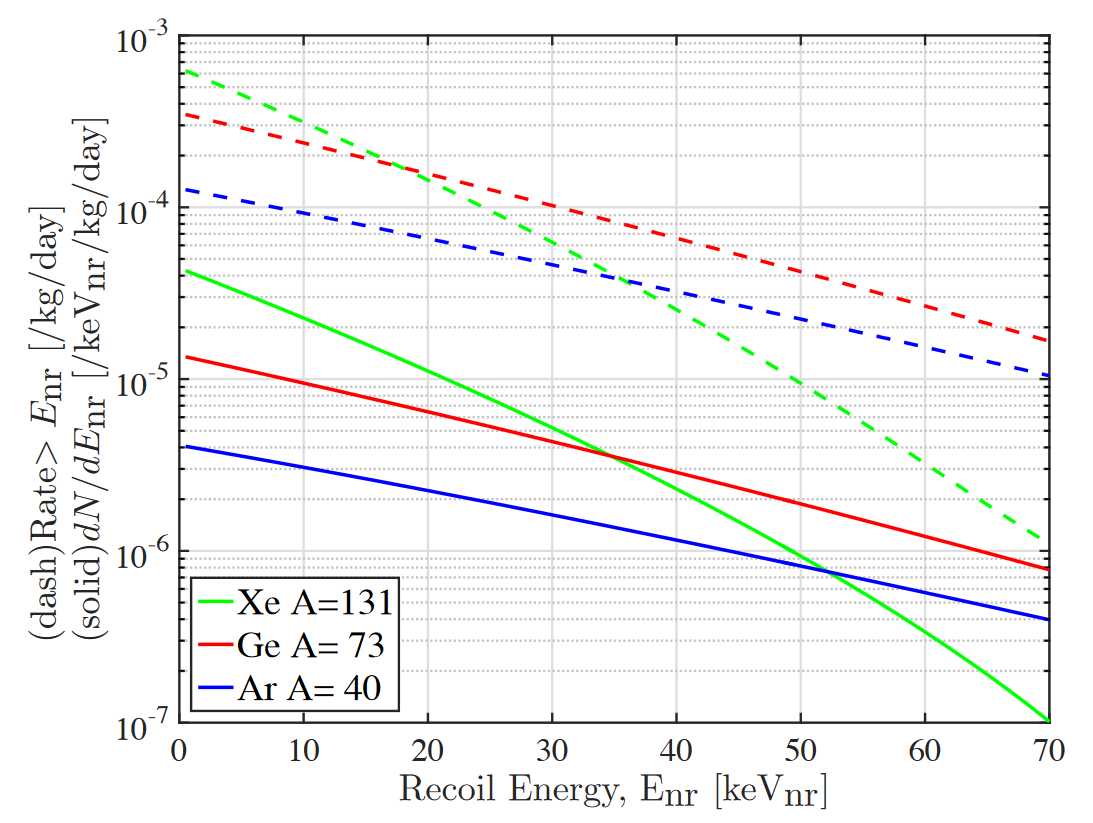
\includegraphics[scale=0.5]{Recoil-spectrum.png}
\captionof{figure}{Calculated differential spectrum in evts/keV/kg/d (solid lines) and the integrated event rate in evts/kg/d (dashed lines)  for $^{131}$Xe, $^{73}$Ge, and $^{40}$Ar assuming a 100 GeV WIMP with spin-indepdent cross section for a WIMP-nucleon of $\sigma=5 \times 10^{-43} cm^2$.}  
\end{center}

Lighter target nuclei will produce lower event rates in a WIMP detector due to their lower cross sections (resulting from lower $A^2$ contribution in the coherent SI term) and less effective transfer of energy during nuclear recoil events. While heavier target nuclei produce stronger interaction cross sections, they also result in reduced event rates at high energies due to a loss of coherence from form factor suppression.  To maximize efficiency a xenon detector with a low analysis threshold is ideal.

%How discrimination is done in cryogenic experiements (CDMS)
%How its done in bubble chambers
%How its done in liquid noble gas
%single phase (pulse shape, with NR producing singlets instead 						of triplet excimers)
%dual phase (NR has higher charge density, so more 							recombination, so lower S2/S1)

\subsubsection{Backgrounds in Direct Detection Experiments} \label{Backgrounds}

%3.4-25 keVnr = 0.9-5.3 keVee over the same S1 range in LUX
Direct detection experiments search for an extremely rare nuclear recoil signal between 1-100 keV.  These detectors have a number of internal and external backgrounds which interfere with the WIMP search signal.  Therefore, limiting sources of background is critical to maintaining a high discovery potential.  

%Reference Paulo's thesis in here somewhere?
Internal backgrounds can be introduced by radioactive materials present in individual detector components.  Naturally occurring radioisotopes such as $^{232}$Th, $^{238}$U, and $^{40}$K can produce high energy gamma rays which penetrate deep into a detector.  In the case of $^{232}$Th, the decay chain produces high energy gamma rays from radioactive daughters such as $^{228}$Ac, $^{212}$Pb, $^{212}$Bi, and $^{208}$Tl before reaching stable $^{208}$Pb.  Likewise, the $^{238}$U decay chain produce high energy gamma rays from $^{234}$Th, $^{234}$Pa, $^{214}$Pb, $^{214}$Bi before reaching stable $^{206}$Pb.  In the case of $^{40}$K, a 1460.85 MeV gamma ray can be produced via electron capture decay to $^{40}$Ar.  In addition to the naturally occurring radioisotopes, cosmogenically activated radioisotopes can also be present inside detector components.  Neutron activation of copper can produce $^{60}$Co, which produces 1.173 MeV and 1.33 MeV gamma rays when it beta decays into $^{60}$Ni via electron emission with a half life of 5.2714 years.  Neutron activation of titanium can produce $^{46}$Sc, which emits 889 keV and 1.12 MeV gamma rays when it beta decays into $^{46}$Ti via electron emission with a half life of 84 days.  Atmospheric radon in the detector introduces the $^{222}$Rn and $^{220}$Rn decay chains as additional backgrounds. While most of the daughters in the radon decay chains produce easily vetoed alpha particles the $^{222}$Rn decay chain includes $^{214}$Pb and $^{214}$Bi.  $^{214}$Pb decays into $^{214}$Bi with a half life of 26.8 minutes via beta emission at 1024 keV, and the subsequent $^{214}$Bi decays in $^{214}$Po with a half life of 19.9 minutes via beta emission at 3272 keV.  The $^{220}$Rn decay chain includes $^{212}$Pb, which decays into $^{212}$Bi with a half life of 10.64 hours via beta emission at 573.8 keV.  The $^{212}$Bi then decays via alpha decay into $^{208}$Tl, which can subsequently decay via beta emission.  These beta decays either produce no gamma ray particles (referred to as "naked" beta decays) or high energy gamma rays that can leave the detector without scattering (refereed to as "semi-naked" beta decays), resulting in a background which can not be reduced via detection of a high energy gamma-ray component.  Internal backgrounds from detector components are mitigated with careful screening of the materials which go into a detector; with simulations being used to predict background events arising from materials which make it through the screening process.
	 	
%LUX Ar39 restraints: Need <1 ppb (g/g) in LUX Xe to be comparable to the $10^{-3}$ events per keV/kg/day background estimate
%LUX Kr85 restraints: Need <20 ppt (g/g) in LUX Xe to be comparable to the $10^{-3}$ events per keV/kg/day background estimate		 
Long lived intrinsic radioisotopes can be present in the detection medium as well.  Cosmogenically activated $^{127}$Xe beta decays via electron capture to $^{127}$I with a half life of 26.358 years.  The captured electron has an 85\% chance of coming from the K shell with an x-ray of 33 keV, a 12\% chance of coming from the L shell with an x-ray of 5.2 keV, and a 3\% chance of coming from higher shells with x-rays of $<$1.2 keV. The subsequent $^{127}$I daughter can decay to ground state via high energy gamma emission, with the gamma frequently leaving the detector without scattering. The $^{127}$Xe activity decays away quickly, so this background can be mitigated by moving the detector underground prior to data collection. $^{39}$Ar is generated by cosmic ray interactions with $^{40}$Ar in a (n,2n) process in the atmosphere and can find it's way into a detector's medium.  The 565 keV electron emission decay has a half life of 269 years, placing strong constraints on the amount of $^{39}$Ar that can be present in a detector's medium when data is collected. $^{85}$Kr is produced by man made processes, such as nuclear fuel processing.  As with $^{39}$Ar, the $^{85}$Kr can make its way into a detector's medium where it will beta decay via electron emission to $^{85}$Rb with a half life of 10.756 years at 687 keV.  These long lived radioisotopes which originate from the atmosphere must be purified from the detector medium prior to data collection to reduce background levels in the detector. \cite{PauloThesis}

Neutrons are particularly dangerous source of background which can mimic the single scatter nuclear recoil present in a WIMP signal.  While neutrons can be stopped by a few tens of meter water equivalent shielding, cosmic ray muons can penetrate many kilometers of shielding.  Muon interactions in the laboratory can produce "cosmogenic" neutrons at the GeV scale with mean free path much longer than most detectors.  These neutrons can be attenuated by rock or shielding and produce keV scale recoils in WIMP detectors.   Such events are mitigated by tagging the initial muon with a muon veto system, placing external shielding around the detector, and by placing the detector deep underground to limit the muon flux.  Neutrons can also be generated internally via ($\alpha$,n) interactions in construction materials, such as the ($\alpha$ + $^{19}$F $\rightarrow$ $^{22}$Na + n) reaction in fluorine present in PTFE, and from spontaneous fission of $^{238}$U and $^{232}$Th.  

The background mitigation techniques discussed in this section can not completely remove backgrounds from a detector.  To separate any remaining backgrounds from a WIMP signal, detectors use a technique called nuclear recoil discrimination.  Nuclear recoil discrimination does not reduce the total number of background events, but instead seeks to distinguish electron recoil interactions from nuclear recoil interactions and reject the former population.  In the next section we discuss a variety of WIMP detection methods, with each of these methods having its own form of nuclear recoil discrimination. 

%Use http://arxiv.org/pdf/1301.0441v1.pdf as a source
\subsubsection{Direct Detection Methods} 
%Get Sources from bradley thesis http://teacher.pas.rochester.edu:8080/wiki/pub/Lux/LuxRequiredReading/AWB_PhDThesis_20140120.pdf
A WIMP deposits energy in a detect in the form of scintillation light, ionization, and heat.  A variety of WIMP detectors have been constructed that each detect one or two of these channels.  Scintillation detectors use scintillating crystals or liquid scintillators as a target medium. For instance, the DAMA/LIBRA experiment at the Gran Sasso Laboratory in Italy uses room temperature, thallium doped sodium iodide (NaI(Tl)) scintillating crystals as a target medium.  Each crystal is paired with two photomultiplier tubes (PMT) which collect scintillation light from within each crystal.  Annual modulation of the WIMP signal due to the motion of the earth around the sun is used to discriminated background events from WIMP events.  The XMASS detector uses liquid xenon as a target medium.  The scintillation produced in the xenon by recoil events is collected by PMT arrays. Background events from gamma ray sources are attenuated by the liquid xenon's large atomic number (Z=54) and high density, leading to a low background fiducial volume.  This discrimination technique is referred to as "self shielding."  Single phase liquid argon experiments, such as DEAP and CLEAN, can not take advantage of self shield techniques due to the intrinsic background from $^{39}$Ar.  Instead, these experiments use a technique called pulse shape discrimination to differentiate signal events from background.  Scintillation in liquid noble gases is produced by the decay of singlet or triplet excimers.  The triplet state emits light over a longer period of time, and the light can be suppressed by destructive interactions such as Penning ionization and electron-triplet spin exchange.  Nuclear recoils produce higher excitation densities, and therefore more destructive interactions with the triplet excimers, leading to a difference in the pulse shape of nuclear recoil and electron recoil events. 

Single phase ionization detectors have also been used in the search for dark matter.  The CoGeNT detector in the Soudan Underground Laboratory in Minnesota uses a low input capacitance p-type point contact (PPC) germanium crystal to detect ionization from WIMP interactions.  The detector has energy thresholds as low as 500 eV, allowing the collaboration to search for low mass ($\sim$5 GeV/c$^2$) WIMP particles.  Electron recoil background events scatter at multiple events sites in the germanium crystal, while WIMPs scatter at most once. This leads to a longer rise time in pulses from background events which can be used as another form of pulse shape discrimination.

Phonon detectors are the final type of single signal detectors.  These type of detectors, such as the Cryogenic Underground Observatory for Rare Events (CUORE) in the Gran Sasso National Laboratory, use low heat capacity crystals as a target medium. In the case of CUORE, tellurium dioxide crystals (TeO$_2$) are held at 10 mK to reduce thermal noise.  The low heat capacity of the crystals allows particle interactions to raise the temperature of the crystals, which in turn changes the resistance of neutron transmutation doped germanium thermistors which are glued to the top of each crystal.  A constant current is applied to the thermistors, and the voltage across each thermistor is used as a detection method.  These types of detectors do not have any means of event discrimination, so they rely heavily on the use of radiopure construction materials and background modeling.

In addition to the single signal detectors, many detectors collect data from two of the three energy deposition channels.  The Cryogenic Dark Matter Search (CDMS)  in the Soudan mine records signals from both phonons and ionization.  The detector uses Ge and Si detectors cooled to $\sim$40mK as a target medium.  The low temperature is required to reduce thermal noise in the detector.  Ionized particles are drifted to the top of the crystals by an electric field where they are read out using field effect transistors, and the corresponding phonon signal is collected by superconducting transition edge sensors coupled with SQUIDs on the opposite face of each crystal.  The ionization yield of a nuclear recoil is lower than an electron recoil, so the ratio of the two signals is used for nuclear recoil discrimination.

The Cryogenic Rare Event Search with Superconducting Thermometers (CRESST) is a phonon and scintillation detector in the Gran Sasso National Laboratory.  CRESST uses calcium tungstate (CaWO$_4$) crystals, which are cooled to 10 mK to lower thermal noise, as a target medium. As with CDMS, transition edge sensors are used to detect phonons originating from particle interactions in the crystals.  Scintillation light in the crystals absorbed by a silicon light absorber that converts the scintillation photons to heat, which are then detected by secondary thermometers.  A nuclear recoil produces 10-40 times less scintillation light in the CaWO$_4$ crystals than an electron recoil does, so the ratio of the phonon and scintillation signal can be used for nuclear recoil discrimination.

The final class of detectors records the scintillation and ionization signals from particle interactions.  These detectors, which are known as dual phase time projection chambers, use liquid noble scintillators (typically xenon) as a target medium. Primary scintillation light is collected by PMT arrays at the top and bottom of the detector. An electric field is used to drift charge from ionized particles to the top of the detector, where the charge produces a secondary source of scintillation light as it accelerates through the gaseous xenon above the liquid.  The ratio of the primary and secondary scintillation light can be used for nuclear recoil discrimination.  Currently, the most sensitive dark matter detector in the world is a dual phase TPC placed in the Sanford Underground Reasearch Facility in South Dakota.  This detector, known as the Large Underground Xenon detector (LUX), will be discussed in depth in chapter \ref{LUXChap}.

\newpage

%	Purity of detector materials in introduction

\section{The LUX Detector} \label{LUXChap} %Talk about self shield in this section
The Large Underground Xenon detector (LUX) is a dual phase time projection chamber location in the Sanford Underground Research facility in South Dakota.  The detector is a dodecagonal structure that uses 300 kg of liquid xenon as a target medium.   The commercially bought xenon was distilled to $\sim$1 ppm (g/g) of air by the manufacturer before undergoing a krypton removal campaign to lower residual krypton levels to less than 5 parts per trillion (g/g).  Particle interactions in the liquid xenon produce ionized and excited state xenon atoms.   Some of the electrons released in the ionization process recombine with the xenon ions, forming additional xenon excitons, while the rest are drifted to the liquid surface by an electric field.   The xenon excitons return to the ground state with a characteristic time constant of 2.2 ns for the singlet state and 27 ns for the triplet state, producing scintillation light at $\sim$175 nm in the processes.  This scintillation light is referred to as the S1 signal.   Electrons which make it to the liquid surface are accelerated through the gas above the liquid xenon by a stronger electric field, producing electroluminescent light which is referred to as the S2 signal. This process will be discussed in depth in section \ref{RecombSec} .

Two arrays of 61 PMTs each are used to measure both the S1 and S2 light in the detector.  The light response of each PMT in the top array is used to reconstruct the XY position of recoil events based on the intensity of the S2 signal, and the time difference between the S1 and S2 signal is used to reconstruct the depth of the recoil events.  In this way, the LUX detector has three dimensional position reconstruction which can be used to construct a low background fiducial volume in the3 center of the detector.  

 \begin{figure} 
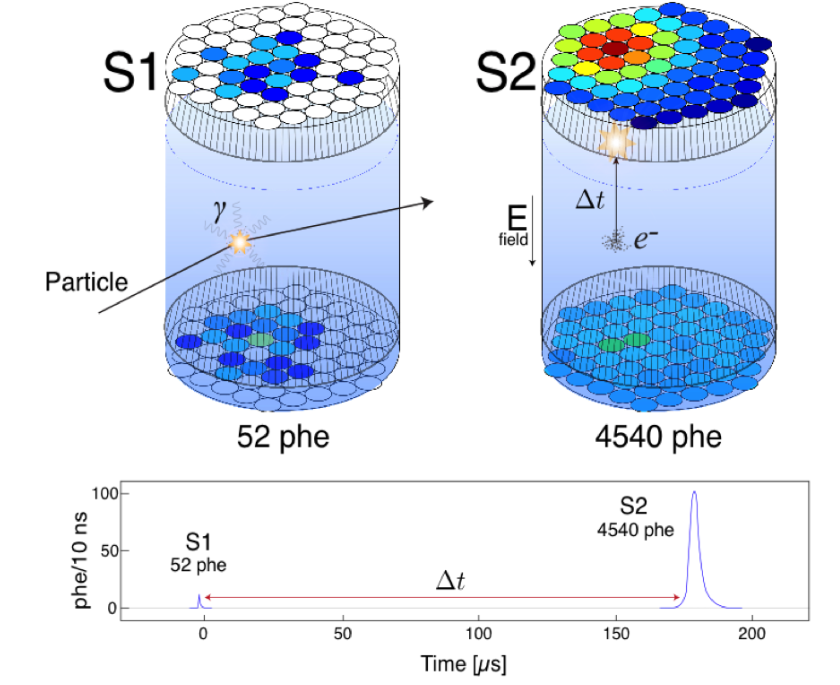
\includegraphics[scale=.5]{LUXevent.png} 
\captionof{figure}{A depiction of a recoil event in LUX. The response of the top PMT array to the S2 light is used for xy position reconstruction, while the timing between the S1 and S2 signals is used for the depth measurement.}
\label{LUXevent}
\end{figure}

The LUX detector is an extremely low background environment due to the strong self shielding properties of liquid xenon and the lack of naturally occurring xenon radioisotopes.  Low energy external backgrounds ($<$50 keV) can only travel a few millimeters into the liquid xenon volume, while higher energy gamma rays ($\sim$MeV range) will produce easily identifiable multiscatter events due to their mean free path of a few centimeters.  Any background events which do appear in the fiducial volume are reduced by over 99\% by using the ratio of the S1 and S2 signal as a form of nuclear recoil discrimination.  Discrimination techniques in the LUX detector will be discussed more in section \ref{DiscrimSec}.  In this section, we will  discuss the detector internals, external support system, and the DAQ electronics used to read out the PMT signal.  

 \begin{figure} 
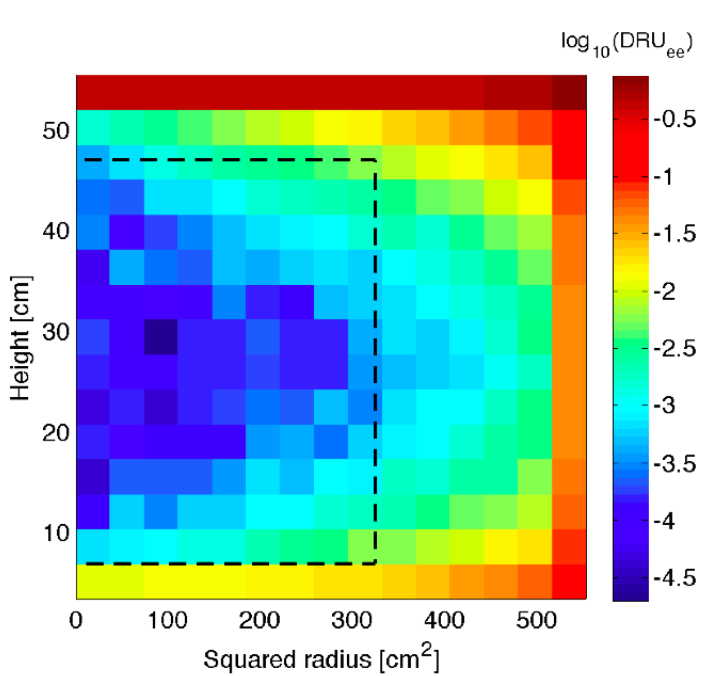
\includegraphics[scale=.5]{GammaBackgrounds.png} 
\captionof{figure}{Simulated gamma ray backgrounds in the LUX detector after removing multiscatter events. The black dashed lines indicate the fiducial volume used in the first LUX WIMP search results.}
\label{GammaBackgrounds}
\end{figure}

\newpage

\subsection{Detector Internals}
\subsubsection{Cryostats} %(Show figure 5 from http://arxiv.org/pdf/1211.3788v2.pdf).


A cross section of the LUX cryostats and detector internals is shown in figure \ref{LuxCross}.  An outer titanium cryostat is used to maintain a thermally insulating vacuum around the detector.  An inner cryostat which houses the liquid xenon and detector internals is attached to the roof of the outer cryostat via three plastic hangers.  Instrumentation cables and gas circulation plumbing are fed through flexible conduits at the top of the detector.  Flexibility of the feedthroughs is required to deal with thermal contraction of the plastic hangers.

 \begin{figure} 
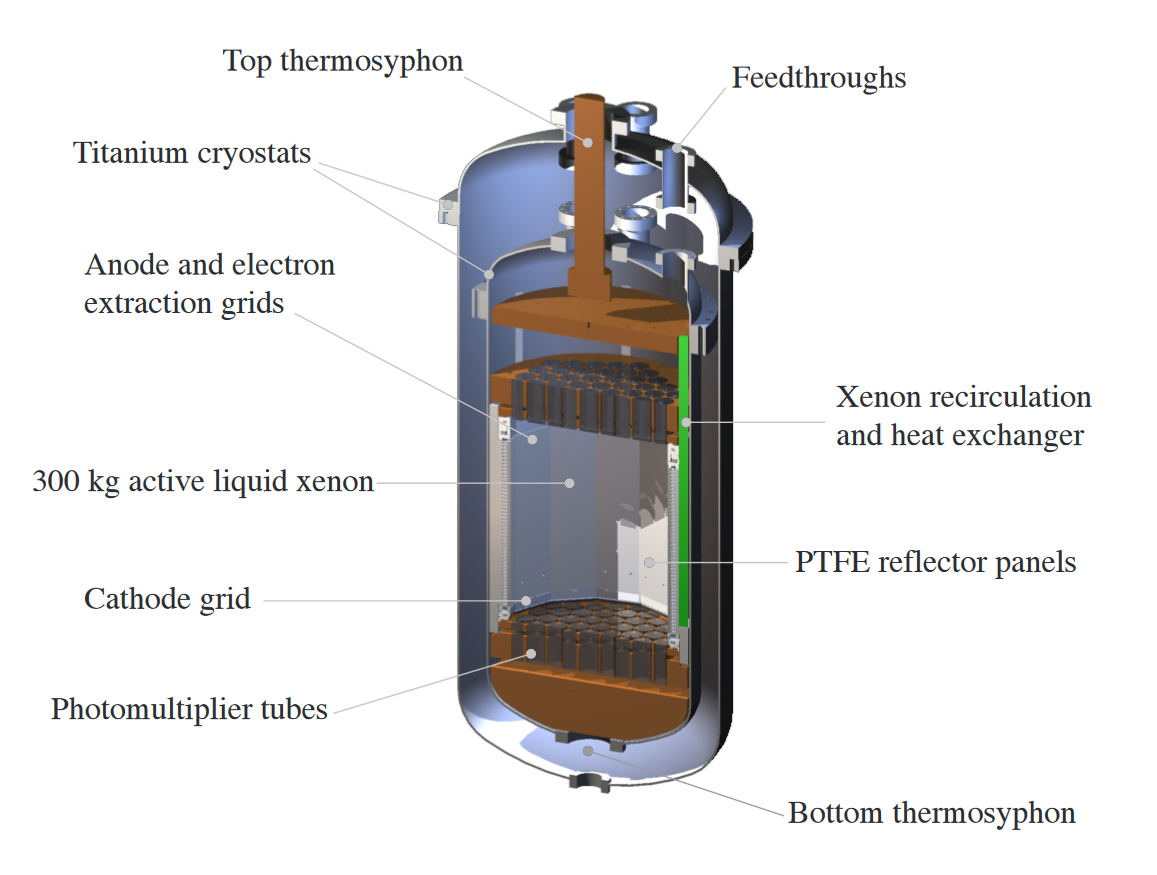
\includegraphics[scale=.45]{LuxCryostat.png} 
\captionof{figure}{Cross section of the LUX cryostats and internal detector components.\cite{LuxDetector}}
\label{LuxCross}
\end{figure}

	
\subsubsection{PMT Arrays, PTFE Structure, and Electric Field Cage}
Inside the inner cryostat, a 5 cm thick copper block with a diameter of 55 cm is mounted directly on to the flange.  This copper serves as a radiation shield and a temperature controller during detector operations. A similar copper structure is attached to the bottom of the inner cryostat and is used to displace xenon from the inactive volume in addition to the functions of the top radiation shield.  

Two PMT arrays are used to collect light from the S1 and S2 signals in the detector.  Each array contains 61 Hamamatsu R8778 PMTs which observe the active volume.  These PMTs were specifically designed for operation in liquid xenon, with a typical quantum efficiency of 33\% at the 175 nm wavelength of liquid xenon scintillation.  The top PMT array is housed in a copper structure which is hung 15 cm below the upper radiation shield by six titanium straps.  Reflective polytetrafluoroethylene (PTFE)   trifoils cover the inner face of the copper housing to increase light collection efficiency in the detector.  A similar structure is placed at the bottom of the detector to house the bottom PMT array. 

Twelve PTFE panels hang from the top PMT support and are attached to the bottom PMT support.  These panels are used to increase light collection efficiency in the detector, and serve as the support structure for the electric field cage in the detector.  The field cage is made of five wire grids.  Each grid is made of thing stainless streel wires and are 88-99\% transparent at a normal angle of incidence.  Stainless steel is known to be 57\% reflective at xenon scintillation wavelength, further minimizing the optical footprint of the wire grids. The top grid is located 2 cm below the top PMT array.  A stainless steel ring is used to string 50 micron diameter stainless steel wires spaced with a pitch of 1 cm.  The voltage on the top grid is used to zero the electric field at the photocathodes of the top PMTs.  The anode is placed 4 cm below the top grid.  It is similar in design to the top grid, but uses 30 micro wires with 0.5 mm spacing. The gate grid, which uses 50 micron stainless steel wires with a pitch of 5 mm, is placed 1 cm below the anode grid. The position of the gate grid places it about 5 mm below the liquid xenon surface.   These two grids work in tandem to produce a strong extraction field (5-6 kV/cm) that pulls charge out of the liquid xenon and into the gas, producing the S2 signal. The cathode grid is placed about 49.5 cm below the liquid surface. This grid uses 260 micron diameter stainless steel wires with a pitch of 5 mm, and works in tandem with the anode grid to produce a $\sim$180 V/cm electric field which drifts charge from a particle interaction to the liquid surface.  The bottom grid is the last of the five wire grids.  It is located 4 cm below the cathode grid and 2 cm above the bottom PMT support, and uses 206 micron diameter stainless steel wires with a pitch of 1 cm.  The bottom grid serves the similar purpose as the top grid – it is used to zero the field at the photocathodes of the bottom PMT arrays.

Fourty-eight copper field rings are spaced 1 cm apart inside of the PTFE panels to shape the drift field. These rings have thickness of 3.2 mm and a width of 12.7 mm.  The spacing and thickness of the rings were chosen to shield the active region from the electric field produced by the cathode high voltage cable.  The voltage of the field rings is set by a resistor chain that runs between the gate and the cathode grids.  A pair of  0.875 G$\Omega$ resistors connect the top field ring to the gate grid, while a pair of 1.25 G$\Omega$ resistors connect the bottom field ring to the cathode grid.  A pair of 1 G$\Omega$ resistors is used to connect each adjacent field ring.


 \begin{figure} [!h]
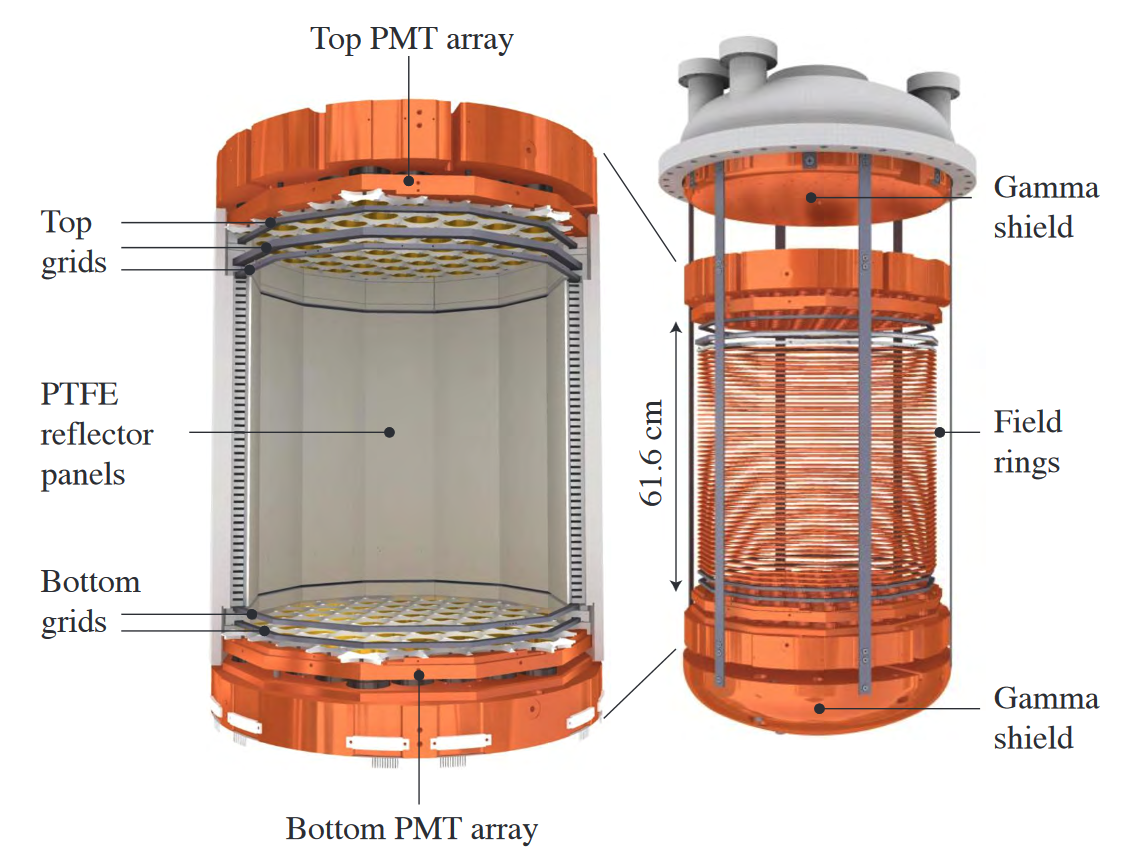
\includegraphics[scale=.45]{LuxFieldCage.png} 
\captionof{figure}{Depiction of the LUX PMT supports, PTFE panels, and field cage.\cite{LuxDetector}}
\label{LuxFieldCage}
\end{figure}


\subsubsection{Cryogenics}

A thermosyphon system is used to cool the detector internals to liquid xenon temperatures  ($\sim$175K) during operation. A thermosyphon is a sealed tube filled with a variable amount of gaseous nitrogen (N$_2$).  A condenser which is immersed in a bath of liquid nitrogen is placed at the top of the thermosyphon.  As the nitrogen in the thermosyphon tube condenses, gravity causes it to trickle down stainless steel plumbing to copper heat exchangers that are attached to various points in the inner cryostat.  The condensed nitrogen evaporates when it hits the copper heat exchanger, removing heat from the detector.  The evaporated nitrogen rises back up the stainless steel plumbing where it is once again condensed by the liquid nitrogen bath.  In this way, the thermosyphons act in a continuous loop, transferring heat from the detector to the liquid nitrogen bath which the condenser is immersed in.

Two thermosyphons are attached to the copper radiation shields at the top and bottom of the inner cryostat and are used as the driving force to cool the detector from room temperature to 175K. Two more thermosyphons are attached to copper shielding around the inner inner cryostat and are used to prevent any thermal gradients from building in the detector.  Each copper evaporator is fitted with a 50 W heater and a thermometer for fine temperature control.  Larger 750 W heaters are attached to the two primary thermosyphons to aid in detector warm up during liquid xenon recovery.

\subsubsection{Instrumentation}

The LUX detectors is fitted with numerous instruments that help monitor and stabilize the conditions within the cryostat. Fourty 100 $\Omega$ thin film platinum resistance temperature detectors (RTDs) are used to monitor the temperature inside the inner cryostat. These instruments are help prevent the formation of thermal gradients which could warp the detector internals.  An additional 23 RTDs are used to monitor the temperature inside the outer vacuum space, providing a means to detect leaks from the inner cryostat or outer atmosphere to the insulating vacuum space. Calibration of the RTD readouts was performed prior to installation, as well as in situ at room temperature, with an accuracy of 170 mK for each RTD.  Advantech Adam 6015 modules are used to feed the output voltage of the RTDs to a slow control database, where multiple users can monitor the read outs and set automated alarms to notify collaboration members of any temperature fluctuations in the detector.  

A variety of pressure sensors are used throughout the detector.  Sensor models include Ashcroft AST4900 sensors, InstruTech Hornet ion and convection gauge, Swagelok PGU-50-PC100-L4FSF manual pressure gauges, and a Setra model 759 capacitance manometer.  These instruments are used to monitor the stability of the inner cryostat, the quality of the outer vacuum, and the pressure in various locations of the gas circulation system.  As with the RTDs mentioned above, all of the digital pressure gauges are read out to the slow control database where alarms can be set to notify users of potential leaks in the circulation system or out of control warming and cooling effects in the detector.

Six parallel wire sensors are used to monitor the liquid level in the inner cryostat, the weir, dual-phase heat exchanger, and the liquid return line.   The later detectors mentioned here will be discussed in section \ref{GasSystem}.  The capacitance of each wire pair depends on the length of wire submerged in the liquid, allowing the overall height of the liquid to be determined.  Additionally, three parallel plate sensors are placed 120 degrees apart between the gate and anode grids.  These sensors ensure the liquid surface is uniform and without any tilt.    


\subsection{External Support Systems}

\subsubsection{Gas Circulation and Purification System} \label{GasSystem}
The xenon used in the LUX detector needs to be free of electronegative and molecular impurities that could attenuate charge and light from particle interactions.  To achieve this goal LUX circulates the detector’s xenon through a gas system which includes a heated zirconium getter made by SAES.  The getter removes nearly all non-nobel gas impurities with an efficiency of 99.9\%, but requires the xenon to be in gaseous form when operating.  

The process of evaporating the liquid xenon, flowing the gaseous xenon to the SAES getter, and recondensing the xenon before to returning it to the inner cryostat is handled by the LUX gas system. Within the inner cryostat excess liquid spills over the lip of a weir into a reservoir, where it enters the evaporator side of a two phase heat exchanger.  In this side of the heat exchanger, xenon is pumped on by the external circulation system until it evaporates. The cooling effect of the evaporation is used to recondense xenon which is returning to the detector on the other side of the heat exchanger, reducing the heat load of the process by 90\%. (\ref{BradleyThesis})

% Xenon produces a flow rate-dependent heat load of 9.8 W/slpm.

The gaseous xenon leaving the evaporator side of the heat exchanger passes through a concentric-tube heat exchanger which warms it to room temperature before circulating to the SAES getter.  After passing through the SAES gettter, the purified xenon continues on to a second concentric-tube heat exchanger where it is cooled before entering the condenser side of the two phase heat exchanger.  After condensing in the two phase heat exchanger the, now liquid, xenon enters the inner cryostat through the bottom radiation shield to ensure its temperature is consistent with the detector internals.

A diaphragm pump which is capable of 50 SLPM (420 kg/day) is used to maintain a constant flow of xenon through the circulation system.  In practice, the flow is limited to $\sim$27 SLPM (227 kg/day) by the output pressure of the circulation pumps. 

%This is directly copied from the section I wrote for the Kr removal paper.  Is it okay to copy and paste my own words from a different paper?
\subsubsection{Gas Sampling System} 

Five xenon sampling ports are including in the gas circulation system.  These ports allow xenon from the two phase heat exchanger, getter input, getter output, conduit purge lines, or circulation pump inlet to be diverted to a xenon assay system.  The assay system makes use of a cryogenic cold trap to separate impurities from the xenon.  During use, a xenon sample flows through the cold trap, where it is frozen through contact with a liquid nitrogen bath.  The frozen xenon sets the vapor pressure of the system at 1.8 mTorr. Most impurities have a vapor pressure higher than 1.8mTorr, allowing them to pass through the cold trap and separate from the bulk of the xenon.  The remaining impurities flow at high leak rates to a commercial Residual Gas Analyzer (RGA) made by SRS, where the absolute level of impurities in the bulk xenon is deduced by comparing to a calibration data set.  After sampling, xenon can be discarded with the use of vacuum pumps in the sampling system, or recovered to high pressure cryogenic storage and recovery vessel (SRV) for potential reuse later.  While we are most concerned with the krypton concentration due to the background producing radioisotope $^{85}$Kr, it is important to assay the other impurities as well.  Argon can produce radioactive backgrounds in the detector, helium can diffuse through PMT faces and damage the vacuum behind them, and nitrogen and oxygen can serve as an indicator for air leaks.  This assaying technique results in sensitivity to krypton below 1 ppt (1e-12) g/g, a factor of 10,000 better than measurements performed without a cold trap.

 \begin{figure} [!h]
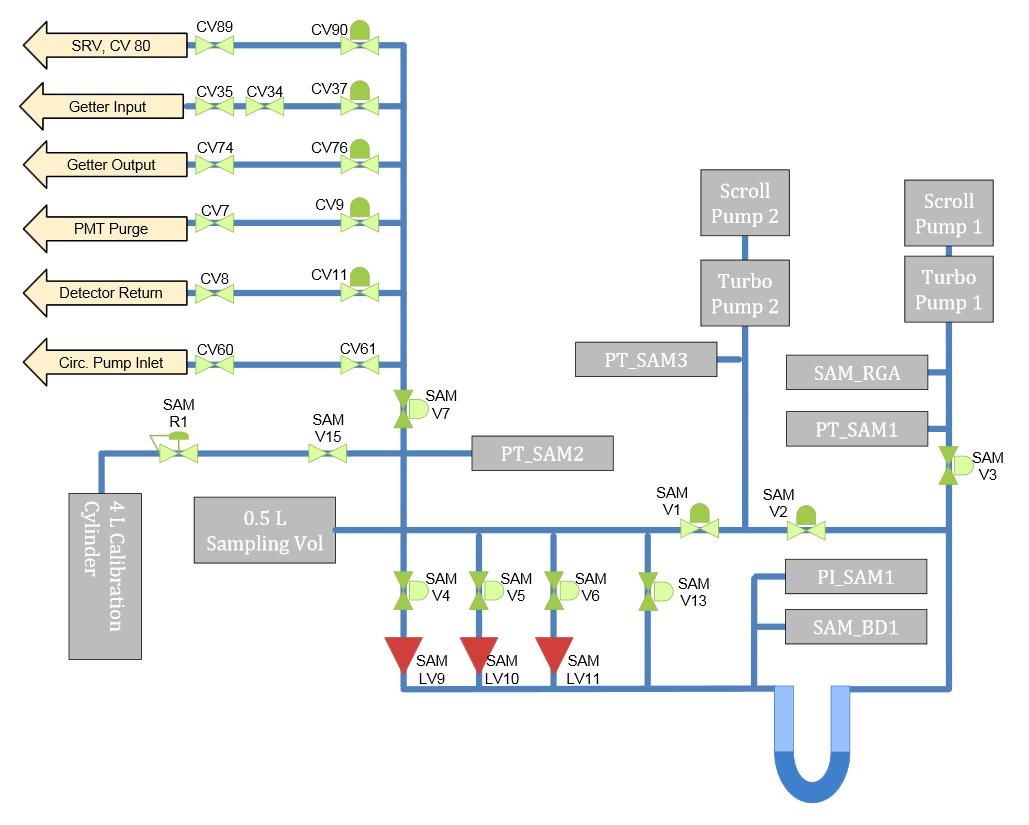
\includegraphics[scale=.3]{SAMdiagram.png} 
\captionof{figure}{Depiction of the LUX sampling system.  Xenon enters the sampling system through various sampling ports in the main circulation path. These sampling ports are shown in the top left of the diagram.  The xenon then passes through one of three leak valves (indicated by red triangles) into a U-shaped cold trap, where it is analyzed by an RGA on the output of the cold trap.  A secondary set of vacuum pumps is included so that the system can be evacuated independently of the RGA space.}
\label{LuxSamSystem}
\end{figure}


\subsubsection{Water Tank and Muon Veto System}

The LUX cryostat is enclosed in a 7.6 meter diameter, 5.1 meter high water tank.  The water tank holds 8 tons of water that is continuously circulated through an industrial purifying system to reduce detector backgrounds originating from the water tank itself.  The concentration of uranium, thorium, and potassium are held more than six orders of magnitude lower than the rock surrounding the laboratory (2 ppt, 3ppt, and 4 ppb respectively). The water tank provides 2.75 m of shielding to the top of the detector, and 3.5 m of shielding to the sides, that reduces backgrounds originating in the laboratory environment.  The tank is also outfitted with 20 Hammamatsu R7081 PMTs which can be used as an active veto for events which coincide with muons passing through the detector.

 \begin{figure} [!h]
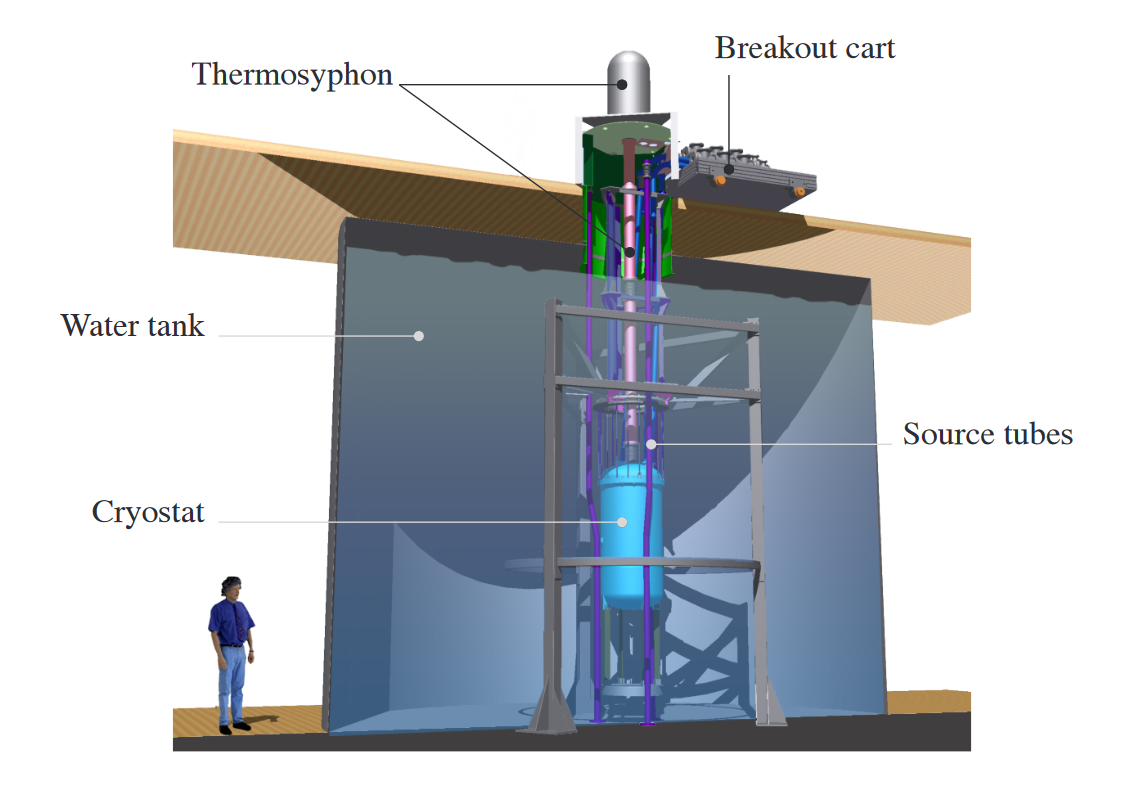
\includegraphics[scale=.35]{LuxWaterTank.png} 
\captionof{figure}{Cross section of the LUX water tank which surrounds the cryostat.}
\label{LuxWaterTank}
\end{figure}

\subsubsection{Calibration Systems}

LUX utilizes multiple internal and external calibration sources to measure the detector's S1 and S2 response to recoil events.  Six source tubes surround the cryostat in the water tank.  A system of pulleys is used to temporarily deploy radioactive sources in each tube.  A collimator is used for directional control of the particle interactions from the external sources. AmBe and $^{252}$Cf are placed in the source tubes to calibrate the detectors nuclear recoil response.  High energy $^{137}$Cs gamma ray sources are placed in the tubes to calibrate the detector's electron recoil response, and to illuminate the detector walls for position reconstruction and background modeling studies.  Other gamma ray sources, such as $^{22}$Na and $^{208}$Tl are available for electron recoil response calibration as well.  High energy gamma rays from external sources only penetrate the outermost centimeters of the liquid xenon volume due the same self shielding properties that reduce unwanted external backgrounds, making it difficult to calibrate the entire fiducial volume with external sources.

\begin{figure} [!h]
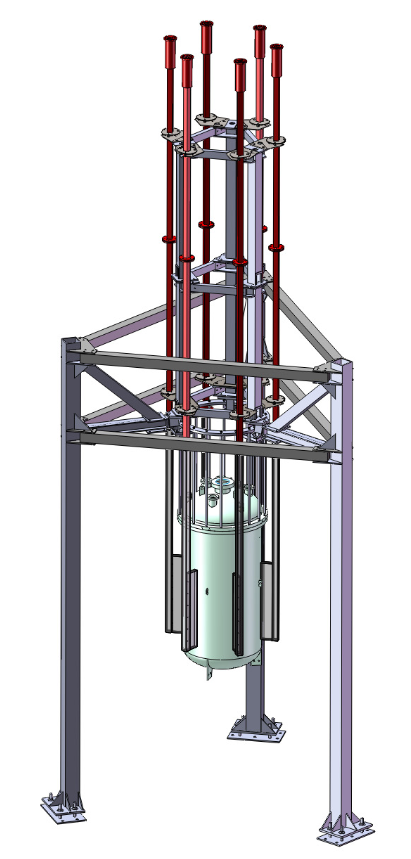
\includegraphics[scale=.35]{LuxSourceTubes.png} 
\captionof{figure}{Rendering of the six external source tubes which surround the LUX cryostat.}
\label{LuxSourceTubes}
\end{figure}

In addition to the source tubes mentioned above, a 377 cm long horizontal air filled conduit can be lowered into the water tank by a pulley system.   This conduit serves to displace water from the tank, opening a collimation path for an Adelphi Technologies,Inc. DD108  deuterium-deuterium neutron generator which is located outside of the water tank.  The neutron generator is operated at a 5\% duty cycle using 100 $\mu$s neutron pulses to produce mono-energetic 2.45 MeV neutrons at a rate of 500 Hz. The resulting neutrons scatter multiple times in the fiducial volume, and are used to calibrate the detector's nuclear recoil response from 0.7 to 24.2 keV$_{nr}$.


LUX also employs two internal calibrations sources which are injected directly into the gas circulation system.   $^{83}$Rb soaked charcoal is used to inject $^{83m}$Kr directly into the circulation system on a weekly basis.  $^{83}$Rb decays into $^{83m}$Kr with an 86.2 day half life.   The resulting $^{83m}$Kr daughter decays via internal conversion at 9.4 keV and 32.1 keV with a half life of 1.86 hours.  Once injected into the gas system, the $^{83m}$Kr quickly makes its way into the fiducial volume, where it uniformly disperses throughout the entire detector.  The spatial uniformity and intrinsic nature of this source makes it extremely useful when measuring the spatial dependence of the detector's S1 and S2 signals, which we will be discuss in depth in Chapter \ref{StandardCalibrations}.  After a calibration has finished, the $^{83m}$Kr is removed from the detector in a short amount of time due to its 1.86 hour half life.  

Tritiated methane (CH$_3$T) is the second internal calibration source used in LUX.  CH$_3$T is a beta source with a peak at 2.5 keV and a mean energy of 5.6 keV.  The wide, low energy spectrum of CH$_3$T is used to calibrate the detector's electron recoil response across the entire energy range of interest for WIMP events.  CH$_3$T has a half life of 12.3 years, so unlike the  $^{83m}$Kr it must be actively removed from the detector by the SAES getter in the circulation system.  The unprecedented CH$_3$T source was designed specifically for LUX, and is discussed in detail in Chapter \ref{TritiumChapter}.


%From: http://xxx.lanl.gov/pdf/1108.1836v2
\subsection{Detector Electronics}

The photons collected by the two PMT arrays are amplified by the PMT dynode chains to mV scale voltage signals.  The rise time for an S1 pulse is limited to $\sim$6 ns by the response of the PMTs, and the 29 ns effective time constant of the xenon excimer relaxation defines the S1 pulses' decay constant.  The pulse width of and S2 event varies with depth due to diffusion of the electron cloud as it drifts through the detector. 

The LUX data acquisition (DAQ) system  is designed to distinguish $>$95\% of single photoelectron pulses at 5 sigma above baseline noise fluctuations, and to prevent saturation of events with energies $<$100 keV$_{ee}$ at any stage in the electronics.  To achieve this, the analog chain must put the peak of single photoelectron distribution at 30 ADC counts.  In the analog chain, the mV scale signals from the PMTs are sent to a x5 amplitude preamplifier before passing to a post amplifier in the DAQ electronics rack. The multichannel post amplifier produces a gain of 1.5x that is sent to sixteen 8-channel ADC modules, and a gain of 2.8x to a DDC-8 trigger system.

The ADC modules digitize the signals at 100 MHz (10 ns/sample) with a resolution of 14 bits. Each ADC board is connected to a VME bus that is subsequently connected to the DAQ computer by fiber optic cables.  Data is downloaded to the DAQ computer with speeds of up to 80 MB/s.  Each ADC board is controlled by four field programmable gate arrays (FPGAs) that operate in a space saving "pulse only digitization" (POD) mode. In POD mode, PMT channels are paired and data is only saved to the DAQ computer if either member of the PMT pairing rises above threshold. A valid pulse trigger gate (VPTG) mechanism further reduces memory space demands.  The VPTG is implemented using CAEN V814 discriminators which require two fold coincidence between PMT channels. Valid pulses are expected to occur in more than one channel, so the VPTG reduces unwanted triggers from various sources of noise.

The DAQ trigger system uses two 8 channel digital signal processors (DDC-8DSP).  
Top and bottom PMTs are summed into 16 groups (8 groups per array), and the analog sum of each group is produced with a Lecroy 628 Linear Fan-In/Fan-Out module.  
A trigger builder is connected to the DDC-8’s and takes $<$1 $\mu$second to generate a final trigger signal to send to the DAQ.  The trigger builder is capable of distinguishing S1 and S2 pulses, and can therefore operate in S1-only, S2-only, or S1 and S2 trigger mode.  The DAQ can operate with a maximum trigger rate of 1.5 kHz before incurring deadtime. 

\subsection{Science Results}

PUT RUN04 RESULT IF (OR RUN03 IF RUN04 ISNT AVAILABLE)


\section{Tritium as a Calibration Source} \label{TritiumChapter}
 
In two phase (liquid and gas) xenon detectors recoil events will produce a scintillation signal (referred to as S1) and ionization. The electrons produced by the ionization process can be drifted to an anode located in the gas phase of the detector. Once the electrons are accelerating toward the anode in the xenon gas they will create a secondary scintillation signal (referred to as S2). Nuclear recoil events have higher ionization density, leading to a higher probability that electron will recombine at the site of the initial recoil event, resulting in a higher S1 yield and lower S2 yield than electron recoil events of the same energy. Therefore, the ratio of the S1 and S2 signals can be used to distinguish electron recoil backgrounds from WIMP-like nuclear recoil events.  This background discrimination technique is referred to as nuclear recoil discrimination.

A detector's response to both nuclear recoil and electron recoil events must be well understood to take advantage of nuclear recoil discrimination.  Typically, an external beta emitter such as $^{137}$Cs is used to calibrate the detector's electron recoil response. However, the xenon in LUX has a strong self-shielding characteristic at UV wavelengths. While this is convenient for eliminating background radiation from external sources, it makes calibrating the innermost regions of the detector difficult with external calibration sources.

To overcome this problem the LUX collaboration is making use of internal calibration sources. An ideal internal calibration source would need to be a single beta emitter in the energy range of interest (< 15 keV) which can be dissolved into the liquid xenon in the detector. Furthermore, the source must be made of a material with low electronegativity so that it will not diminish the drift length of charge in the detector. Similarly the source cannot attenuate the UV scintillation light produced by events in the detector. To achieve a reliable calibration in all regions of the detector the source would need to have a long enough life time to diffuse throughout the entire detector (a few hours). Finally, there must be a method for removing the source once the calibration has finished. This could simply mean waiting for the source to decay if its half life is short, or actively purifying the source out of the detector if its half life is long

Tritium meets several of these requirements. It is a beta emitter with a Q-value of 18 keV, a mean energy of 5.6 keV, and a mode 3 keV that produces a broad spectrum over the entire energy range of interest. Its 12.3 year half life means that the source will have plenty of time to dissolve uniformly throughout the detector. However, this long half life is potentially dangerous, since one can not simply wait for it to decay away { it must be actively
removed from the detector when the calibration is completed. To complicate this matter bare tritium sticks to most surfaces, including materials like teflon, polyethylene, and steel which make up the majority of most xenon detectors. To make tritium removal more feasible we have made use of tritiated methane(CH$_3$T). Methane is highly inert due to its fully saturated carbon-hydrogen bonds. It has a diffusion constant in polyethylene that is 10 times smaller than
hydrogen, and it does not capture electrons that will be drifting through the detector. By replacing one of the hydrogen atoms in a methane molecule with tritium we combine the strength of both of these materials, resulting in the ideal internal calibration source.

\subsection{Tritiated Methane Injection System}

The design of our triated methane calibration technique can be separated into three parts: the injection system, the tritiated methane source bottle, the zirconium getter.

The tritiated methane source bottle was prepared in three steps. First, we prepared a xenon bottle that had similar pressure and purity to the LUX system. We filled a 2250 cc stainless steel bottle with 1590 torr of xenon from the same dekryptonation and purity
program which the LUX xenon came from. The purpose of this xenon was to serve as a carrier gas for the tritiated methane. The next step was to prepare a small amount of tritiated methane to mix with
this dekryptonated xenon. A reservoir of tritiated methane with an activity of 204 Bq/torr-cc was purchased from Moravek Biochemical. The reservoir was frozen with liquid nitrogen, resulting in a vapor pres-
sure of 10.4 $\pm$ 0.05 torr. We then opened the frozen tritiated methane reservoir to a 1/4" VCR cross which was sealed with swagelok valves on each side. This first expansion space had a total volume of 5.2 $\pm$ 0.9 cc. Next, we isolated the VCR cross from the tritiated
methane reservoir and then opened it to a 501 $\pm$ 0.2 cc expansion volume. We isolated the VCR cross a second time and then opened it up to a 53.2 $\pm$ 3.4 cc expansion volume. The VCR cross was then isolated for a third time before opening it to a 10.5 $\pm$ 0.5 cc expansion volume. After this final expansion the VCR cross was isolated and the remaining 0.016 $\pm$ 0.006 torr-cc of tritiated methane left within was mixed with the dekryptonated xenon inside the 2250 cc bottle via cryopumping. The final result was a tritiated methane source which had an activity of 9.1e-7 $\pm$ 3.4e-7 Bq/torr-cc.  After the success of the initial CH$_3$T calibrations in LUX, a similar procedure was used to produce stronger source bottles for higher statistics calibrations.

The injection system for our tritiated methane calibration technique consists of a series of expansion volumes which are used to fine tune the amount of CH$_3$T that is injected. Once the CH$_3$T source bottle is opened it flows through a methane gas purifier (SAES MC1-905F) to remove any sources of potential contamination, such as bare tritium. The CH$_3$T then flows into the expansions volumes set by the
user. We use expansion volumes of 9.8 $\pm$ 0.4 cc, 13.3 $\pm$ 0.4 cc, 26.0 $\pm$ 0.5 cc, 82.7 $\pm$ 0.5 cc, 12.0 $\pm$ 0.6 cc, and 132.7 $\pm$ 0.6 cc in setup, which provide over an order of magnitude control in the strength of an injection. Note that each injection will lower the total activity in the CH$_3$T source bottle via volume sharing, results in a smaller, yet calculable, injection activity with subsequent injections. Once the expansion volumes
have filled, the flow of xenon in the gas system is diverted through the expansion volumes to sweep the CH$_3$T into the detector. We continue to flow through the expansion volumes for one hour at 1 SLPM, which is equivalent to flushing out the full 384.5 cc of the expansion volumes roughly 75 times. Two pump out ports allow various parts of the injection system to be evacuated in preparation for each use. A pressure gauge (PT-T1) is included above the tritiated methane source
bottle so that this drop in activity can be measured. The final component of the injection system is a particle filter (Mott Corp. GSP3752FF11) which prevents particles contaminants from entering the LUX detector.

\begin{figure} [!h]
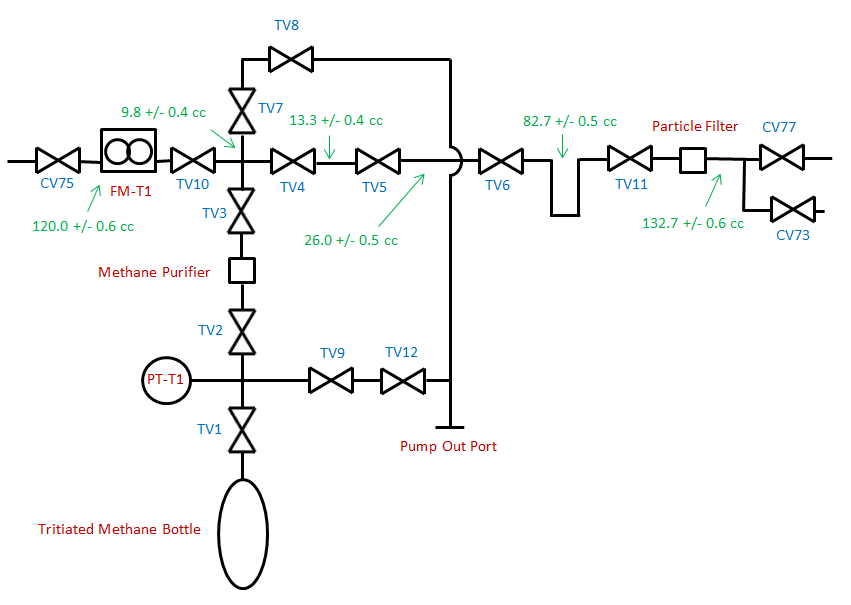
\includegraphics[scale=.6]{TritiumPlumbing.png} 
\captionof{figure}{Plumbing diagram of the LUX tritium injection system.  Blue labels indicate valves, red labels indicate equipment, and green labels indicate the size of individual expansion volumes when all valves are closed.}
\label{LUXInjectionSys}
\end{figure}

Once the CH3T has been injected in the LUX gas system it flows into the liquid xenon
inside of the LUX cryostat, where it diffuses uniformly throughout the fiducial volume.  The CH$_3$ inside of the cryostat beta decays, producing electron recoil events over a wide range of energies throughout the entire detector.  

Since the xenon gas in LUX is constantly circulating, the remaining CH$_3$T is swept out of inner cryostat with the circulating xenon.  The LUX gas system uses a hot zirconium getter (SAES ??) downstream of the cryostat to remove CH$_3$T and other impurities from from the xenon. Extensive R\&D was conducted using a smaller zirconium getter (SAES pcf4c3r1) at the University of Maryland to learn about the CH$_3$T removal efficiency of these purifiers. Details of these studies is discussed in section \ref{UMDRemoval}.

\subsection{Triated Methane Removal} \label{UMDRemoval}

To study the CH$_3$T removal efficiency of zirconium getters the University of Maryland built two separate systems to inject tritiated methane into a gaseous xenon
and a liquid xenon environment. Both of these systems used zirconium getters to
remove any CH$_3$T that was injected into them.

\subsubsection{Gas Phase Experiments}

The gaseous xenon system consists of three sections. The first section, the
xenon space, contains a hot zirconium getter to remove CH$_3$T from the system, two xenon storage bottles used to move xenon through the system via cryopumping, and a proportional tube used to detect activity within the xenon space. The second section is a small transfer system which is used to inject consistent amounts of CH$_3$T into the xenon space with each injection. The final section consists of a CH$_3$T storage bottle used as the source of injections and a SAES MC1-905F methane purifier to remove unwanted contaminates prior to entering the xenon space.

%Insert gas system diagram here
\begin{figure}
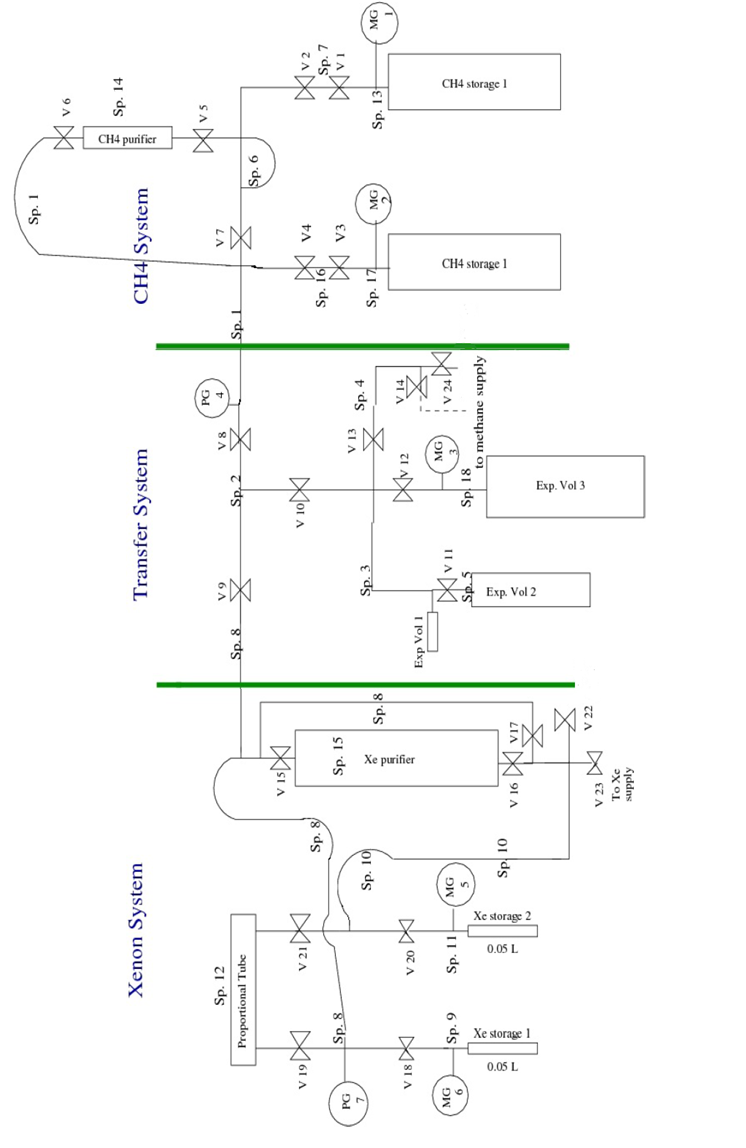
\includegraphics[scale=.55]{GasSystem.png} 
\captionof{figure}{Diagram of the gaseous xenon system at UMD.  THe three section of the system are distinguished by green lines.  Circles labeled PG and MG are pressure gauges, and the hourglass shaped symbols represent hand valves.}
\label{UMDGasSystem}
\end{figure}

The primary goal of this experiment was to determine the purification efficiency of the zirconium getter and study residual contamination. We found that the flow rate through the getter and the amount of time between injections had the largest impact of purification efficiency.  High  flow rates through the purifier can cool the zirconium inside, while inadequate rest time between subsequent purifications can lead to build up of methane on the surface of the zirconium beads. Both of these situations lead to a decrease in purifier efficiency. The first black data point in Figure \ref{UMDGasFlowRate} is our worst purification efficiency, (96\% $\pm$ 1\%) corresponding to our highest flow rate. (8 SLPM compared to the typical 0.3 SLPM) While we were unable to control the  flow through rate as much as we desired, we are at least able to conclude that exceeding the maximum flow rate suggested for the purifier does significantly decrease purification efficiency. We also found that allowing ample rest time between subsequent purifications significantly increases purification efficiency. Our best purifications were the first data points in each cluster in Figure \ref{UMDGasRestTime}. We were able to obtain efficiencies of 99.99\% when the purifier was resting for three weeks or longer, and obtained efficiencies ranging from 99.00\% to 99.90\% when the purifier was
used on a daily basis.

\begin{figure}
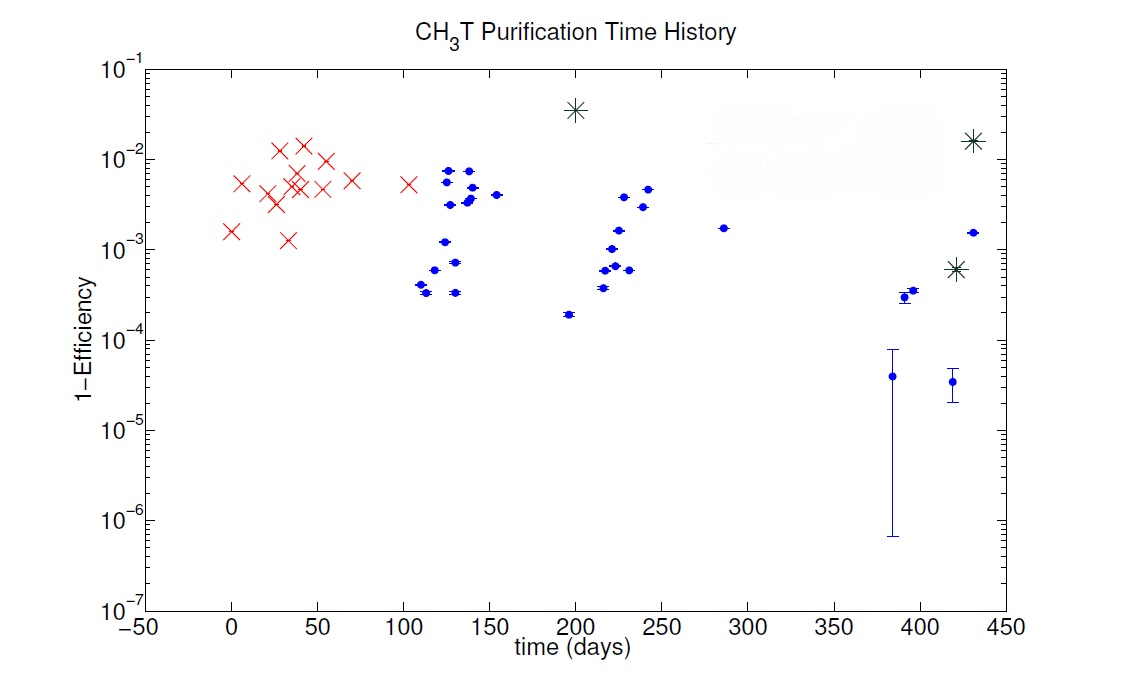
\includegraphics[scale=.45]{GasPhaseRemoval_FlowRate.jpg} 
\captionof{figure}{Single pass inefficiency of the purifier when removing CH$_3$T.  Red and blue points indicate data taken by different students, while the black points indicate data for which procedures were intentionally altered.}
\label{UMDGasFlowRate}
\end{figure}

\begin{figure}
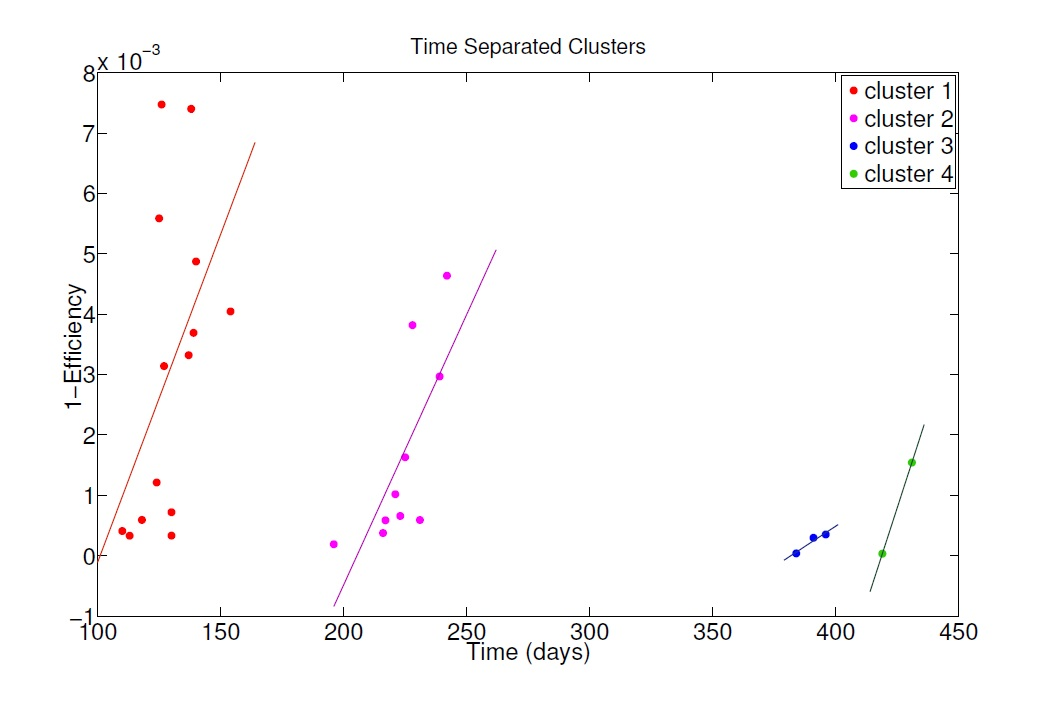
\includegraphics[scale=.4]{GasPhaseRemoval_RestTime.jpg} 
\captionof{figure}{Time-separated clusters of purification have an upward trend in purification inefficiency.}
\label{UMDGasRestTime}
\end{figure}



\subsubsection{Liquid Phase Experiments}

We have also tested tritium removal from liquid xenon. Our liquid xenon system
consists of three main sections, the CH$_3$T injection system, the xenon circulation system, and the liquid xenon cryostat. We will first discuss the set up of the tritium injection system, pictured below. The injection system begins at the CH$_3$T storage bottle. This bottle is double valved for safety reasons. As with the gaseous experiments, we have a SAES MC1-905F methane purifier in series with the storage bottle. Following the methane purifier there is a series of injection volumes branching out to the left. These injection volumes are designed to inject the desired amount of CH$_3$T into the xenon system. The last component of the injection system is located above the injection volumes. This plumbing is used to collect all of the CH$_3$T from the injection volume via cyropumping. After the plumbing has warmed, the xenon circulating outside of the injection system is rerouted through the cryopump plumbing to sweep all of the CH$_3$T into the xenon circulation system. 


\begin{figure}
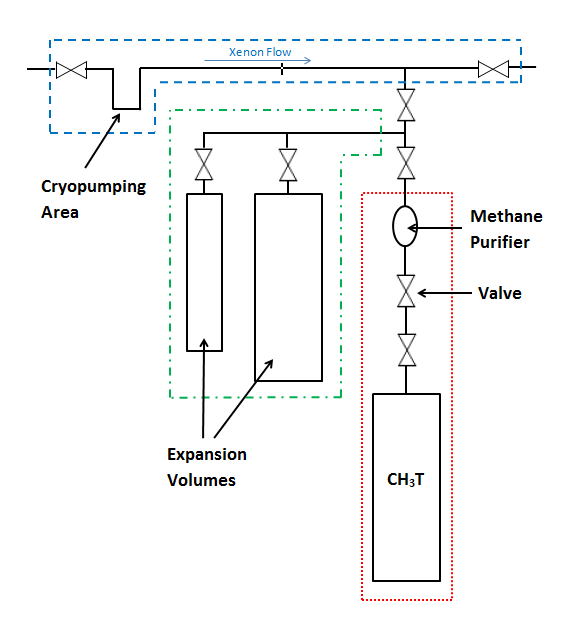
\includegraphics[scale=.6]{UMDInjectionSys.png} 
\captionof{figure}{The tritium injection system for the liquid phase experiments at UMD. The red box indicates the CH$_3$T storage bottle and methane purifier area, the green box indicated the expansion volumes, and the box indicates the cryopumping and xenon flow through area.}
\label{UMDInjectionSystem}
\end{figure}


In the xenon circulation system, a small diaphragm pump circulates gaseous xenon in a close circuit.  A zirconium getter (SAES pcf4c3r1) is positioned in between the CH$_3$T injection system and the liquid xenon cryostat.  A bypass around the zirconium getter is present to allow control of when CH$_3$T removal occurs.

The final section of our system, the liquid xenon cryostat, is pictured in Figure \ref{UMDcryo}. In the liquid xenon system, a pulse tube refrigerator cools a xenon gas condenser consisting of a helical coil of copper tubing. The condensed xenon drips into a liquid xenon storage vessel. Two PMTs are placed inside of the storage vessel to observe scintillation light produce by CH$_3$T decays in the liquid xenon. Once the vessel is filled both of these PMTs are submerged in the liquid xenon. Note that this means the system at UMD is a single phase detector, rather than a dual phase detector like LUX. Polyethylene and teflon curtains were installed in the inner cryostat to surround the PMTs during some of our data sets. These curtains of plastic were used to study outgassing effects in our detector.

\begin{figure}
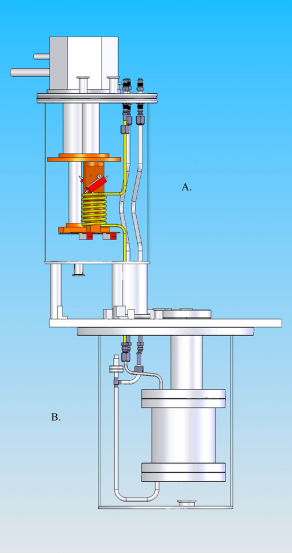
\includegraphics[scale=.45]{UMDCryo.png} 
\captionof{figure}{The liquid xenon system at UMD. (A) The xenon condenser consists of a helical coil cooled by a pulse tube refrigerator. (B) The liquid xenon storage vessel houses two PMTs to observe tritium decay.}
\label{UMDcryo}
\end{figure}


During our liquid phase experiments, our experimental procedure consisted of
taking an adequate amount of background data, injecting CH$_3$T into the liquid xenon, waiting for the CH$_3$T event rate to plateau, and then purifying the CH$_3$T
out of the xenon. During the data sets in which teflon or polyethylene curtains
were installed around our PMTs we bypassed our purifier after initially purifying
away the CH$_3$T so that outgassing effects could be studied. Injection activities for our liquid phase experiment ranged from 1487 $\pm$ 35.06 Bq to 12164 $\pm$ 1028.11 Bq.
A detailed list of our purification efficiency measurements in liquid xenon is
included in Table \ref{UMDPurification}. Note that the rise in background rate during our polyethylene runs is due to a change in PMT gain. Using the lessons learned from the gaseous xenon experiments we were able to achieve an average purification efficiency of 99.999\% in our liquid experiments, where we define our purification efficiency to be 

\begin{equation}
\text{Purification Efficiency} = 1 - \frac{A-B}{I-B},
\end{equation}

where A is the background event rate after injecting CH$_3$T, B is the background event rate before to injecting CH$_3$T, and I is the injected CH$_3$T activity as observed by out PMTs. We find that the addition of plastic curtains around our PMTs does not impair our ability to remove CH$_3$T at > 99.998\% levels. To illustrate the effectiveness of CH$_3$T removal, an overlay of injected and purified CH$_3$T spectra is included in Figure \ref{BeforeAndAfterSpec}. Cumulatively, we have injected over 68,000 observed becquerel of CH$_3$T into our liquid xenon. Although systematic errors lead to a fluctuation of our residual background rates, we see no upward trend in our data set as the cumulative observed injection activity rises.(Figure \ref{UMDBackgroundOverTime})


\begin{figure}
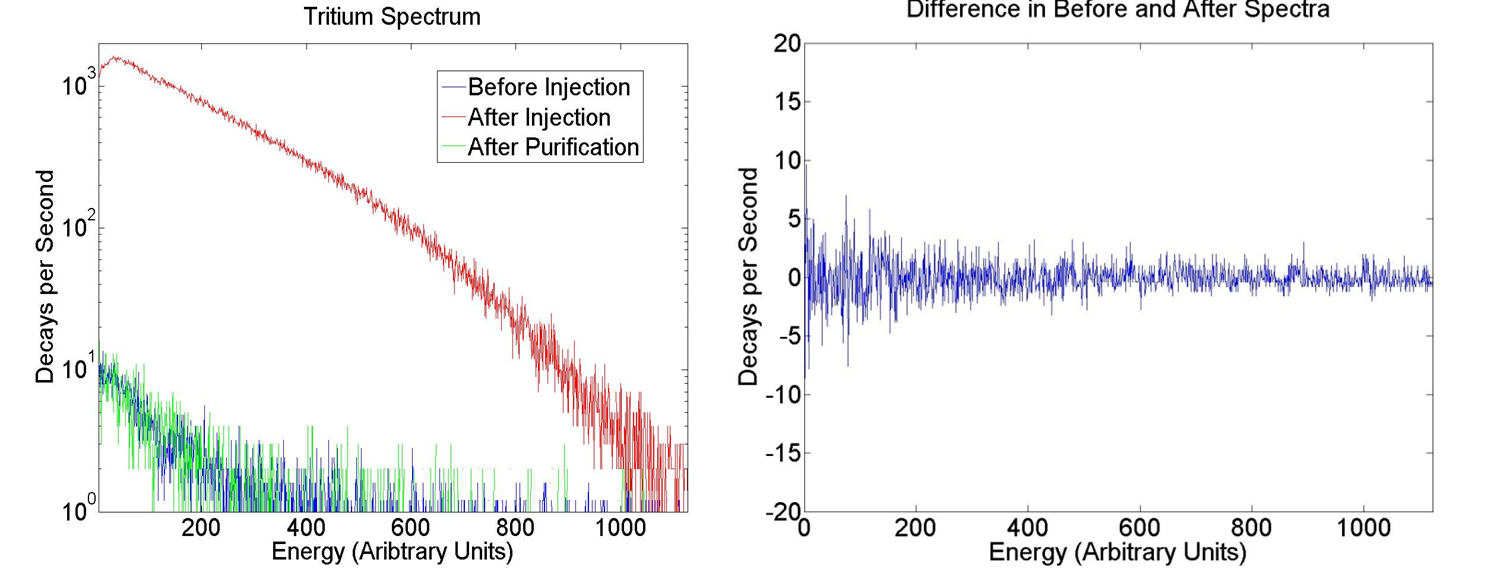
\includegraphics[scale=.5]{UMDspectra.png} 
\captionof{figure}{Left: Overlay of CH$_3$T spectra seen by PMTs in the liquid xenon detector. The blue spectrum is what is seen prior to injecting tritium, the red spectrum is what is seen after injecting tritium, and the green spectrum is what is seen by after purifying the xenon to remove any injected CH$_3$T. Right: The difference between the before injection and after purification spectra.}
\label{BeforeAndAfterSpec}
\end{figure}

\begin{figure}
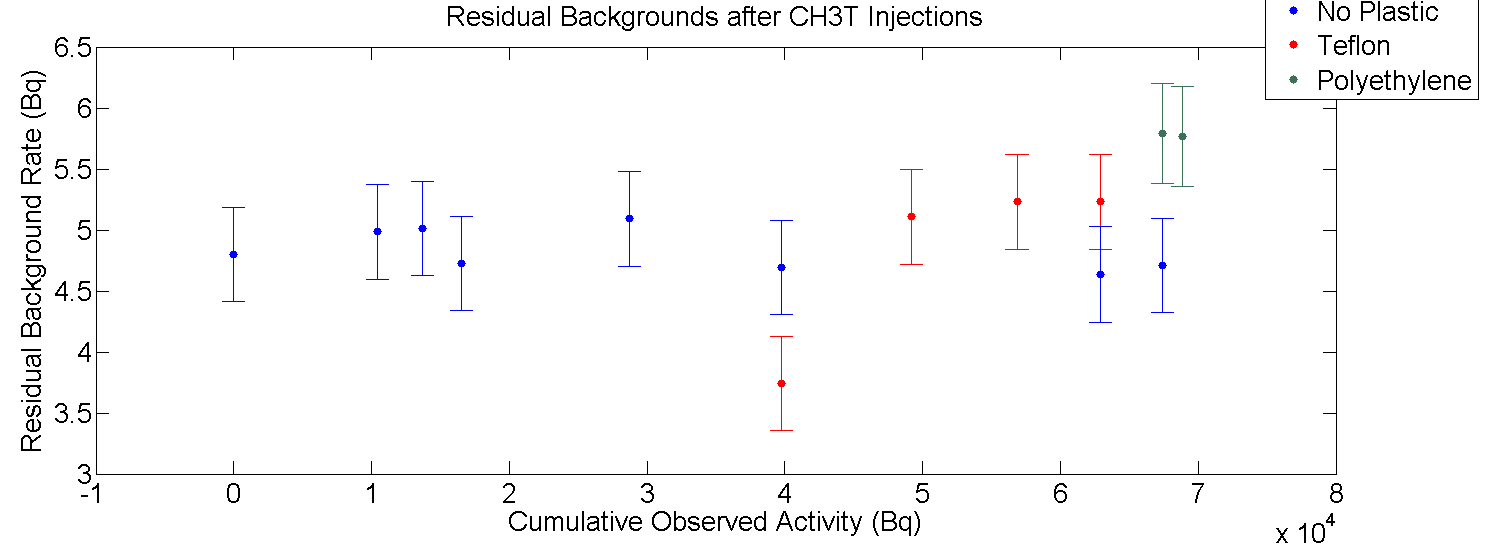
\includegraphics[scale=.35]{ResidualBackgroundCorrected_SystemErr.png} 
\captionof{figure}{Residual background rates over time in the UMD detector after purifying the CH$_3$T out of the xenon. Blue data points are data sets in which no plastic curtains were used inside of the detector, red data points are data sets in which teflon curtains were
used inside of the detector, and green data points are data sets in which polyethylene curtains were used inside of the detector.}
\label{UMDBackgroundOverTime}
\end{figure}

\begin{sidewaystable}
\scalebox{0.9}{
\centering
\caption{CH$_3$T purification efficiencies in liquid xenon.} \label{UMDPurification}
\begin{tabular}{ c | c | c | c | c }
Observed Injection Activity (Bq) & Background Before Injection (Bq) & Background After Injection (Bq) & Purification Efficiency & Type of Plastic \\
\hline
10415.84 $\pm$ 140.89 & 4.78 $\pm$ 0.38 & 4.99 $\pm$ 0.39 & 0.99998 $\pm$ 0.000054 & No Plastic \\
3295.15 $\pm$ 46.28 & 4.99 $\pm$ 0.39 & 5.01 $\pm$ 0.39 & 0.99999 $\pm$ 0.00017 & No Plastic \\
2836.67 $\pm$ 22.35 & 5.01 $\pm$ 0.39 & 4.76 $\pm$ 0.39 & 1.00009 $\pm$ 0.00020 & No Plastic \\
12164.29 $\pm$ 1028.11 & 4.72 $\pm$ 0.39 & 5.09 $\pm$ 0.39 & 0.99997 $\pm$ 0.000082 & No Plastic \\
11033.62 $\pm$ 1766.87 & 5.09 $\pm$ 0.39 & 4.69 $\pm$ 0.38 & 1.00004 $\pm$ 0.00015 & No Plastic \\
9435.13 $\pm$ 180.13 & 3.74 $\pm$ 0.38 & 5.32 $\pm$ 0.39 & 0.99983 $\pm$ 0.000061 & Teflon \\
7666.08 $\pm$ 226.67 & 5.11 $\pm$ 0.39 & 5.23 $\pm$ 0.39 & 0.99998 $\pm$ 0.000082 & Teflon \\
6043.72 $\pm$ 446.80 & 5.23 $\pm$ 0.39 & 5.23 $\pm$ 0.39 & 1.00000 $\pm$ 0.00016 & Teflon \\
4504.81 $\pm$ 220.89 & 4.64 $\pm$ 0.39 & 4.71 $\pm$ 0.40 & 0.99998 $\pm$ 0.00016 & No Plastic \\
1487.09 $\pm$ 35.06 & 5.79 $\pm$ 0.41 & 5.76 $\pm$ 0.41 & 1.00002 $\pm$ 0.00043 & Polyethylene \\
\end{tabular}
}
\end{sidewaystable}


\subsubsection{Outgassing Experiements} 

To more accurately model the LUX detector we surrounded our PMTs with polyethylene or teflon panels during some of our data sets. The experimental procedure for these data sets was to collect an adequate amount of background data, inject CH$_3$T into the liquid xenon, wait for the CH$_3$T event rate to plateau, purify the CH$_3$T away until we reached the initial background event rate, then bypass the purifier on our system to study outgassing effects. Once the purifier had been bypassed we discovered two sources of residual CH$_3$T contamination. We see a gradual rise in CH$_3$T activity after bypassing our purifier due to outgassing of CH$_3$T from the plastic panels.  This outgassing effect will be discussed in detail in Section \ref{SimOutgas}. In addition to this steady rise, we see large steps in CH$_3$T activity at random intervals. (Figure \ref{UMDOutgassing}) These step features occur every 3 days on average. The longest period of time without a step occurring was 5.08 days. To examine these step features more closely, we analyzed the spectra from one of these events. We found that the integral of the spectra rose from 8833 $\pm$ 93.98 to 17190 $\pm$ 131.11 during the event, an increase of 194.6\%. (Figure \ref{UMDOutgassingSpectra})

\begin{figure}
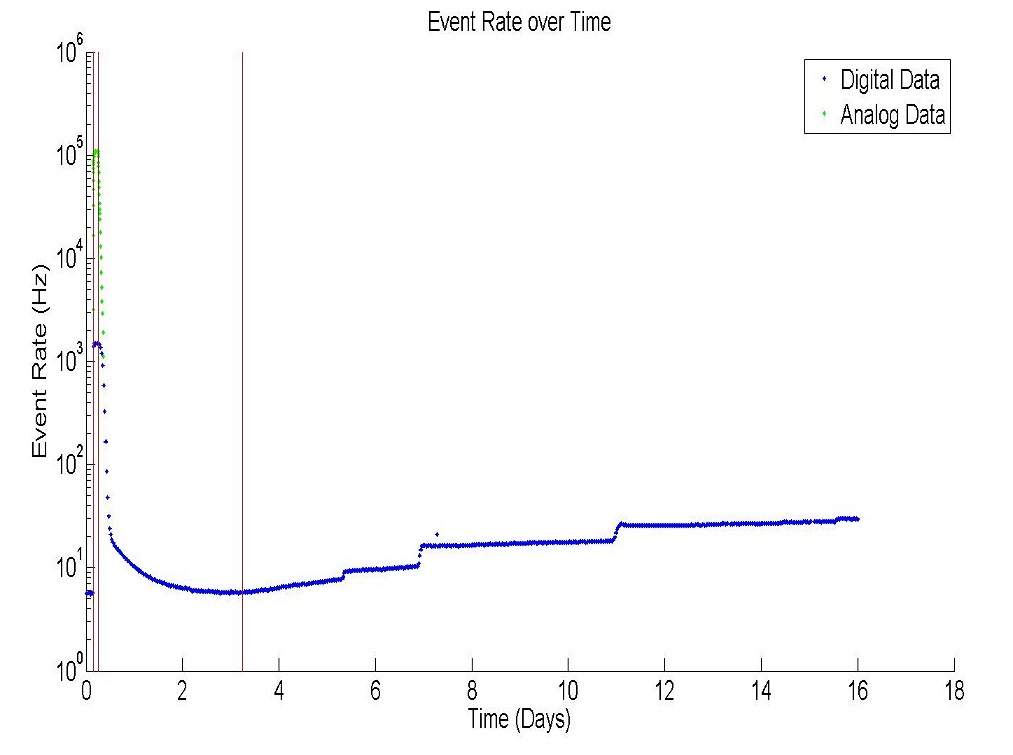
\includegraphics[scale=.35]{Outgassing_TimeHisto_Log.jpg} 
\captionof{figure}{A time histogram of the CH$_3$T rate in our system. The third red line indicates when our purifier was bypassed.}
\label{UMDOutgassing}
\end{figure}

\begin{figure}
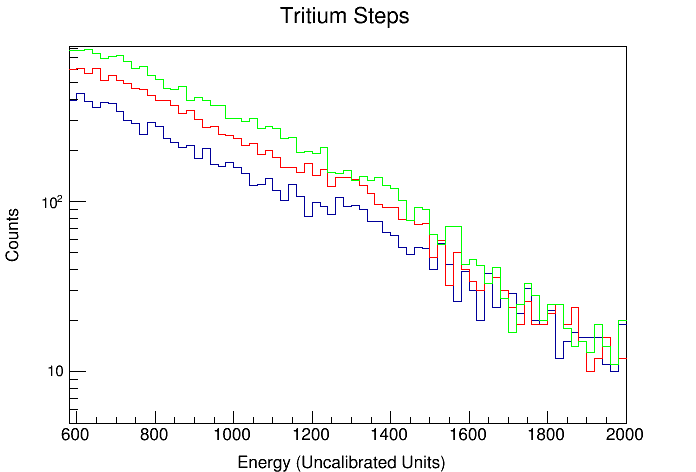
\includegraphics[scale=.35]{Steps_Overlay.png} 
\captionof{figure}{An overlay of three spectra from a step in CH$_3$T after bypassing our purifier. The blue spectrum was collected prior to a step occurring, the red spectrum was collected while a step was occurring, and the green spectrum was collected after the step had reached a plateau.}
\label{UMDOutgassingSpectra}
\end{figure}

Such an increase in CH$_3$T activity can be produced through two mechanisms: a drift in PMT gain which would shift the CH$_3$T spectrum horizontally, or an increase in CH$_3$T activity shifting the CH$_3$T spectrum vertically. To determine if our PMT gain was shifting during our CH$_3$T data sets we used an external $^{137}$Cs source. Over eight days the $^{137}$Cs event rate remained flat, with an initial event rate of 120255 $\pm$ 346.778 observed Bq and a final event rate of 115469 $\pm$ 339.807 observed Bq. A linear fit to the $^{137}$Cs data results in a nearly zero slope of 0.0026 Bq per day. (Figure \ref{UMDCsData}) We conclude that the rise in tritium rate during the step events can not be due to our PMT gain drifting, and must therefore be a result of an increase in the amount of CH$_3$T in the fiducial region of our detector. We suspect this increase in CH$_3$T is due to pockets of stagnant gas slowly moving into the detector's fiducial region. To avoid such a source of residual CH$_3$T contamination, a detector wishing to using tritiated methane as an internal calibration source must be designed such that no areas of stagnant gas exist within its system.  

\begin{figure}
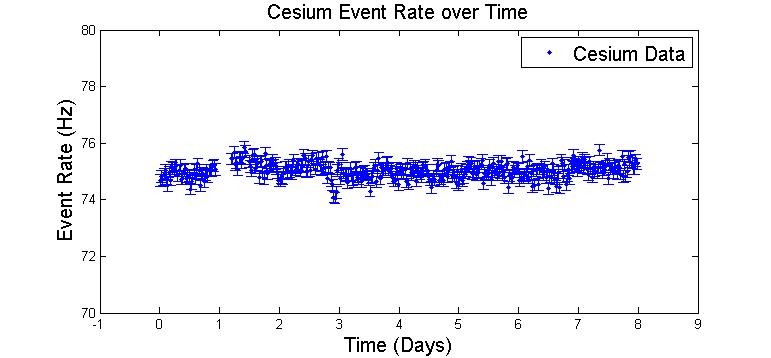
\includegraphics[scale=.35]{Cesium_TimeHisto.jpg} 
\captionof{figure}{The event rate of a $^{137}$Cs source placed outside the xenon storage vessel.  The flatness of the rate over time indicates that the PMT gains are mostly constant.}
\label{UMDCsData}
\end{figure}

\subsubsection{Simulating Outgassing in LUX} \label{SimOutgas}

The outgassing effects seen in UMD's small scale liquid xenon experiment places an upper limit on the CH$_3$T activity that can be injected into low background detectors such as LUX.   In the LUX collaboration we chose to define the tolerable CH$_3$T activity after a calibration to be 5\% of the nominal background rate in LUX, setting a limit on the residual CH$_3$T activity of 0.33 $\mu$Bq.  This upper limit is extremely conservative, and guarantees that any electron recoil backgrounds introduced by a CH$_3$T calibration will be negligible. 

With the above constraints in mind, we can determine an upper limit on the amount of CH$_3$T that can be injected for internal calibrations of the LUX detector. The diffusion process is governed by two different equations known as Fick's laws. Fick's first law describes the flux of a material through a surface. Its general form is given by
\begin{equation}
J=-D\frac{d \phi(r,t)}{d r}.
\end{equation}
Combining Fick's first law with the continuity equation given by
\begin{equation}
\frac{\delta \phi}{\delta t} + \nabla \cdot J = 0,
\end{equation}
which states that a change in density in any part of the system is due to inflow and outflow of material results in Fick's second law,
\begin{equation}
\frac{\delta \phi}{\delta t} = D \nabla^2 \phi,
\end{equation}
which describes the transport of a material by diffusion.

To implement these diffusion laws into our model we must determine the diffusion coefficient of CH$_3$T in the plastics of LUX. At room temperature, the diffusion coefficient of methane in teflon is measured to be $2.3 \times 10^{-7} \frac{cm^2}{sec}$. \cite{MethaneDiffusion}.  The temperature dependence of this diffusion constant is modeled by the Arrhenius equation,  
\begin{equation}
D=Ae^{\frac{-E_a}{RT}}
\end{equation}
where $E_a$ is the activation energy, $R$ is the gas constant, and $T$ is the temperature.  This suggests than an adjustment factor to the diffusion constant of $10^6$ at liquid xenon
temperature. This adjustment factor is equivalent to increasing the thickness of the plastic in our model by a factor of 1,000. For this reason we are motivated
to use half-infinite line boundary conditions in our diffusion model.

The analytic solution to Fick's second law using half-finite line boundary conditions is
\begin{equation}
\phi(x,t) = KC_{out} - \int_0^t \text{erf}\left(\frac{x}{\sqrt{4D(t-\tau))}}\right)K \dot{C_{out}}(\tau)d\tau - KC_{out}(0)\text{erf}\left(\frac{x}{\sqrt{4Dt}}\right)
\end{equation}
where $K$ is the solubility of the material and $C_{out}$ is the outside concentration of the material.  \cite{FicksAnalytic}  For the outgassing process we are only interest in the flux of the material out of the plastic.  This is given by Fick's first law evaluated at $x=0$,
\begin{equation}
J_{out}(t)=-K\sqrt{\frac{D}{\pi}} \left( \int_0^t \frac{\dot{C_{out}(\tau)}}{\sqrt{t-\tau}}d\tau + \frac{C_{out}(t)}{\sqrt{t}} \right),
\end{equation}
where the sign has been flipped since the flux of material is outward. We see that it is no longer possible to evaluate $K$ and $D$ separately, since the diffusion in and out of the plastic is completely determined by the time-dependent concentration outside of the plastic. To simplify our model, we define a new constant
\begin{equation}
G=K\sqrt{\frac{D}{\pi}}
\end{equation}
We can fit the integral of our equation for the flux out of the plastic over time to the outgassing data collected in Maryland's liquid xenon system to extract a value for the constant $G$. Since the outgassing data includes step features from stagnant pockets of unpurified CH$_3$T, we can set an upper limit on $G$ by assuming the step features are a result of outgassing itself, and a lower limit on $G$ by removing the steps from our data, treating them as if they have no connection to outgassing at all. With this method
we loosely constrain $0.0001 \frac{cm}{\sqrt{day}} \le G \le 0.0075  \frac{cm}{\sqrt{day}}$. (Figure \ref{StepsandNoSteps}) The value of G was further constrained to $G \le 0.0002 \frac{cm}{\sqrt{day}}$ by injecting natural methane into LUX and observing the effects of outgassing with the sampling system. 

\begin{figure}
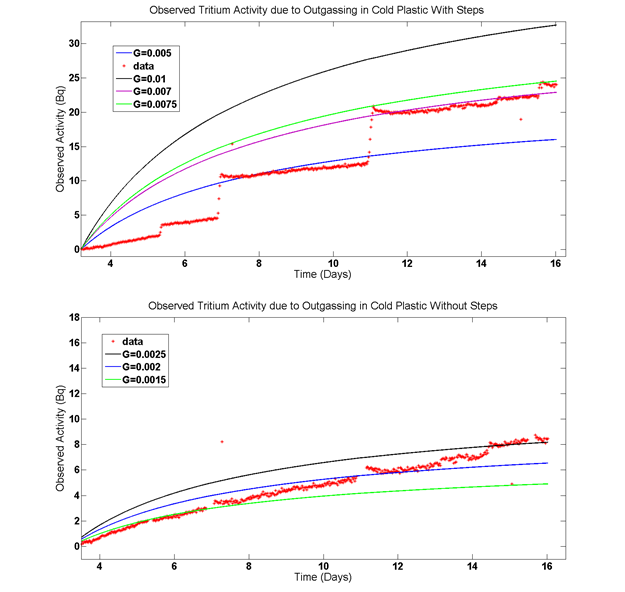
\includegraphics[scale=.7]{StepsandNoSteps.png} 
\captionof{figure}{Fits of the integral of the flux of CH$_3$T out of plastic over time to the outgassing data collected in Maryland's liquid xenon system assuming that the step features
are due to diffusion. The model does not perfectly describe the data, so a range of $G$ values is shown. These fits are used to
set an upper limit on $G$. Bottom: Fits of the integral of the flux of CH$_3$T out of plastic over time to the same data, assuming that the step features are not due to diffusion. These fits are used to set a lower limit on $G$.}
\label{StepsandNoSteps}
\end{figure}


With a constraint on G taken from the analytic solution to Fick's second law, we turn to numerical simulation to answer
the question of how much initial CH$_3$T activity to inject into LUX to meet our calibration conditions. Several assumptions are made to simplify the numerical model. First, we approximate the diffusion into plastic as being a one dimensional process. In cylindrical coordinates, Fick's laws become
\begin{equation}
J = -D \left( \frac{\delta \phi}{\delta r} \mathbf{\hat{r}} + \frac{1}{r} \frac{\delta \phi}{\delta \theta} \boldsymbol{\hat{\theta}} + \frac{\delta \phi}{\delta z} \mathbf{\hat{z}} \right) 
\end{equation}
\begin{equation}
\frac{\delta \phi}{\delta t} = D \left( \frac{\delta^2 \phi}{\delta r^2} + \frac{1}{r}\frac{\delta \phi}{\delta r} + \frac{1}{r^2} \frac{\delta^2 \phi}{\delta \theta^2} + \frac{\delta^2 \phi}{\delta z^2} \right).
\end{equation}
Since the plastic in our detector at Maryland and in LUX can be approximated by a cylindrical shell, there is no dependence on the azimuthal or z coordinates. Since $r$ is large compared to the thickness of the plastic shell, $\frac{\delta^2 \phi}{\delta r^2} \gg \frac{1}{r}\frac{\delta \phi}{\delta r}$, so we can make the approximations
\begin{equation}
J=-D\frac{\delta \phi}{\delta r} \mathbf{\hat{r}}
\end{equation}
\begin{equation}
\frac{\delta \phi}{\delta t} = D \frac{\delta^2 \phi}{\delta r^2}
\end{equation}

We assume the concentration of CH$_3$T in LUX is uniform throughout its volume. This assumption is justified, since the design of LUX creates currents which stirs the liquid xenon. With perfect mixing the effect of the purifier can be modeled by adding an exponential time dependence to the outer volume. The time constant of this decay is equal to the time it takes xenon to recirculate through the LUX detector. We use a simple implementation of the first order Euler method for our numerical simulations. The finite difference approximations of Fick's two laws in one dimension are
\begin{equation}
J_{i,j}=-D \frac{ \phi_{i+1,j} - \phi{i,j}}{\Delta x}
\end{equation}
\begin{equation}
\phi_{i,j+1}=\phi_{i,j}+ \Delta t \left( \frac{\phi_{i+1,j}-2\phi_{i,j}+\phi_{i-1,j}}{\Delta x^2}\right)
\end{equation}
where $i$ is the spacial index and $j$ is the time index.  To avoid divergence solutions we need
\begin{equation}
D\frac{\Delta t}{\Delta x^2} \le \frac{1}{2}.
\end{equation}
For effects to be propagated across N spacial bins, N time steps are required.
Therefore, the effective time resolution is
\begin{equation}
\Delta t_{\text{effective}}=\Delta t \times N_x.
\end{equation}

The diffusion is simulated by setting the concentration at the boundary of the piece equal to $KC_{out}$, where $C_{out}$ is the concentration of CH$_3$T in the xenon. This concentration is dependent on time according to
\begin{equation}
\frac{\delta C_{out}}{\delta t} = J_{out} \frac{A_{\text{plastic}}}{V_{\text{xenon}}}-\frac{C_{out}}{\tau}
\end{equation}
where $A_{\text{plastic}}$ is the surface area of the
plastic cylinder, $V_{\text{xenon}}$ is the total volume of xenon in the fiducial region, and $\tau$ is the time it takes for one full purification cycle. It was original assumed that $\tau$ would equal the turn over time of the xenon circulation system in LUX ($\sim$ 1.3 days), but was later found that $\tau$ was much shorter than expected ($\sim$ 6 hours). The first term on the right of this equation models outgassing of CH$_3$T from the plastic cylinder, while the second term models removal of CH$_3$T through purification. Using the first order Euler method, we arrive at an expression for $C_{out}$ given by
\begin{equation}
C_{j+1}=C_j + \Delta t \left[\left( J_{1,j}-J_{N_x,j}\right) \frac{A_{\text{plastic}}}{V_{\text{xenon}}} - \frac{C_j}{\tau} \right].
\end{equation}

The initial concentration is defined by dividing the desired injection activity by the volume of the fiducial region. We choose $D = 2.3 \times 10^{-9} \frac{cm^2}{sec}$ such that the
half-infinite boundary conditions in our diffusion model is valid, and combine this with our allowed range of values for $G$ to extract a value for $K$. We find that an initial injection activity of 10 Bq results in the background rate returning to $<$ 5\% of its initial value in one month. \cite{JonOutgassing} (Figure \ref{OutgassingSim})

\begin{figure}
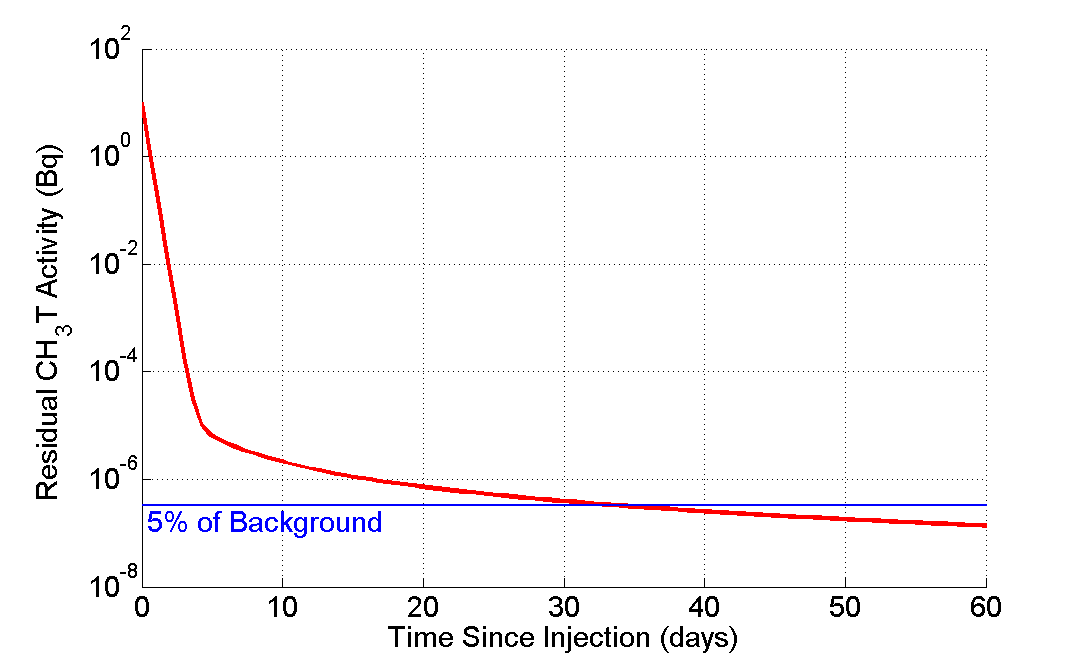
\includegraphics[scale=.3]{OutgassingSim.png} 
\captionof{figure}{The results of simulating the CH$_3$T activity in LUX after a 10 Bq injection.  In the first week the amount of residual CH$_3$T is dominated by the purification time constant, while the out gassing time constant determines the amount of activity later times.}
\label{OutgassingSim}
\end{figure}

\subsection{ER Band Calibration of the LUX Detector} 

The LUX collaboration took many precautions to ensure a safe and successful tritium injection. Prior to injecting any tritiated methane into the detector, a natural methane injection was preformed to measure the purification time constant in LUX and constrain the value of $G$ further.   Twenty milligrams of natural methane were injected into LUX using the CH$_3$T injection system. The sampling system was used to measure the concentration of methane in the detector over the next few days, and a purification time constant of 5.90 $\pm$ 0.07 hours was measured.  The first natural methane injection was not large enough to observe outgassing from the detector, but a larger natural methane injection of 0.375 grams was able to constrain $G \le 0.0002 \frac{cm}{\sqrt{day}}$ at a later date.


\begin{figure} [!h]
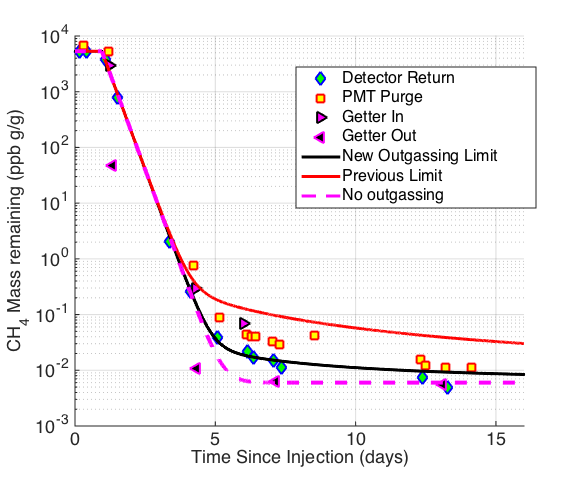
\includegraphics[scale=.7]{LUXOutgassing.png} 
\captionof{figure}{Sampling system results from the 0.375 gram natural methane injection which was used to constraint the value of $G$. \cite{JonOutgassingTwo}}
\label{LuxOutgassing}
\end{figure}

After the natural methane campaign a small amount of tritium was injected into LUX to confirm the purification time constant from above, and to confirm the mixing of the source throughout the detector.  A fiducial volume containing 125 kg of xenon between drift times of 30 to 320 $\mu$sec, with radius $ < $17.5 cm was defined for the analysis.  The first 23 hours of data show that the initial injection activity in the fiducial volume was 24.2 $\pm$ 0.3 mBq, while the initial injection activity in the entire detector was 44.9 $pm$ 0.5 mBq.  The ratio of the fiducial volume activity to the total volume activity is 0.539 $\pm$ 0.009, which is close to the expected ratio of 0.5 for a perfectly uniform distribution of CH$_3$T events. The CH$_3$T activity fell with a purification time constant of 6.9 $\pm$ 0.4 hours within the fiducial volume, confirming the $\sim$ 6 hour time constant measurement from phase one.

\begin{figure} [!h]
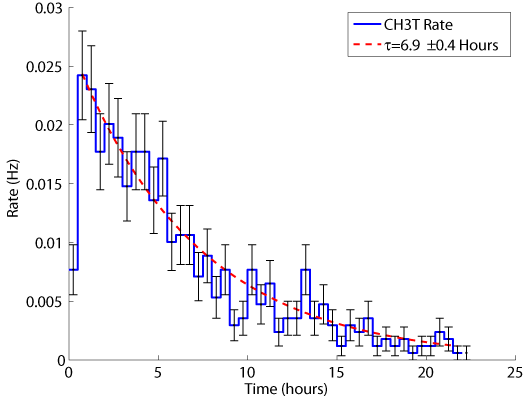
\includegraphics[scale=.7]{CH3T_fid_rate_new.png} 
\captionof{figure}{Rate of CH$_3$T events after the first small injection into LUX.  The 6.9 hour time constant is consistent with expectations from the natural methane sampling campaign prior to this injection.}
\label{LUXPurificationRate}
\end{figure}

After confirming the purification time constant LUX approved the use of CH$_3$T as an internal calibration source.  The initial CH$_3$T calibration was limited to 0.3 Hz due to the uncertainty in the value of the the diffusion constant $G$, but injections ranging from 2-10 Hz have been done every 3-4 months after the value of $G$ was constrained further.  The location of events from the first CH$_3$T calibration is shown in Figure \ref{TritiumSpatialDist}. As expected, the CH$_3$T source diffuses uniformly throughout the detector.  
\begin{figure} [!h]
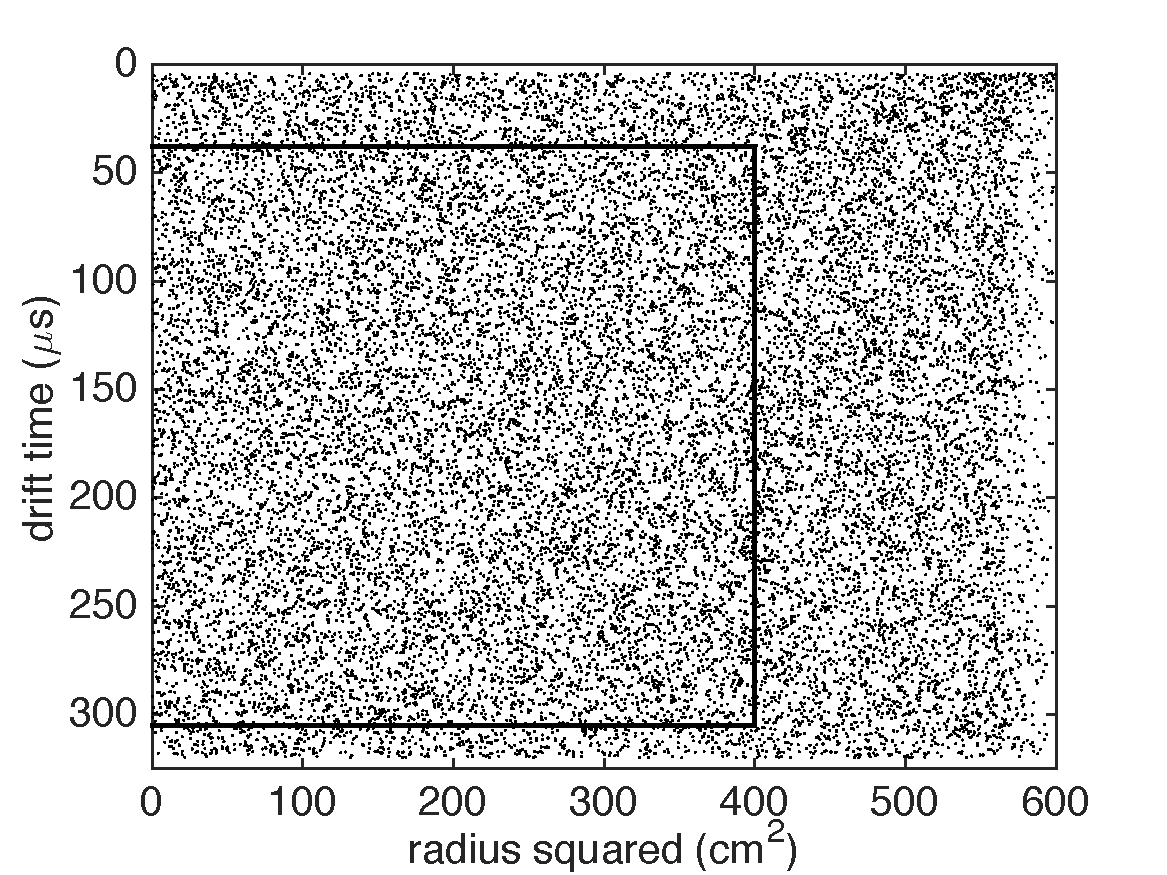
\includegraphics[scale=.5]{TritiumRvZ.pdf} 
\captionof{figure}{The location of events during the initial LUX CH$_3$T injection.  The solid black like indicates the fiducial volume used for the first LUX Run03 results paper.}
\label{TritiumSpatialDist}
\end{figure}

The combined energy spectrum for a high statistics CH$_3$T calibration is shown in Figure \ref{TritiumSpectrum}.  A model of the expected tritium beta spectrum which includes detector resolution effects is shown in red.  The data agrees very close with expectations above the detector's energy threshold, with a p-value of 0.70 from 3 to 18 keV.  The consistency of the energy spectrum across a wide range of energies provides strong support for the combined energy model presented in Section \ref{CombinedEnergyModel}.  The ratio of the CH$_3$T data to expectations was used to determine the energy threshold of the LUX detector.  A error function fit was used to determine a 50\% energy threshold of 1.24 $\pm$ 0.026 keV for electron recoil events.

\newpage

\begin{figure} [!h]
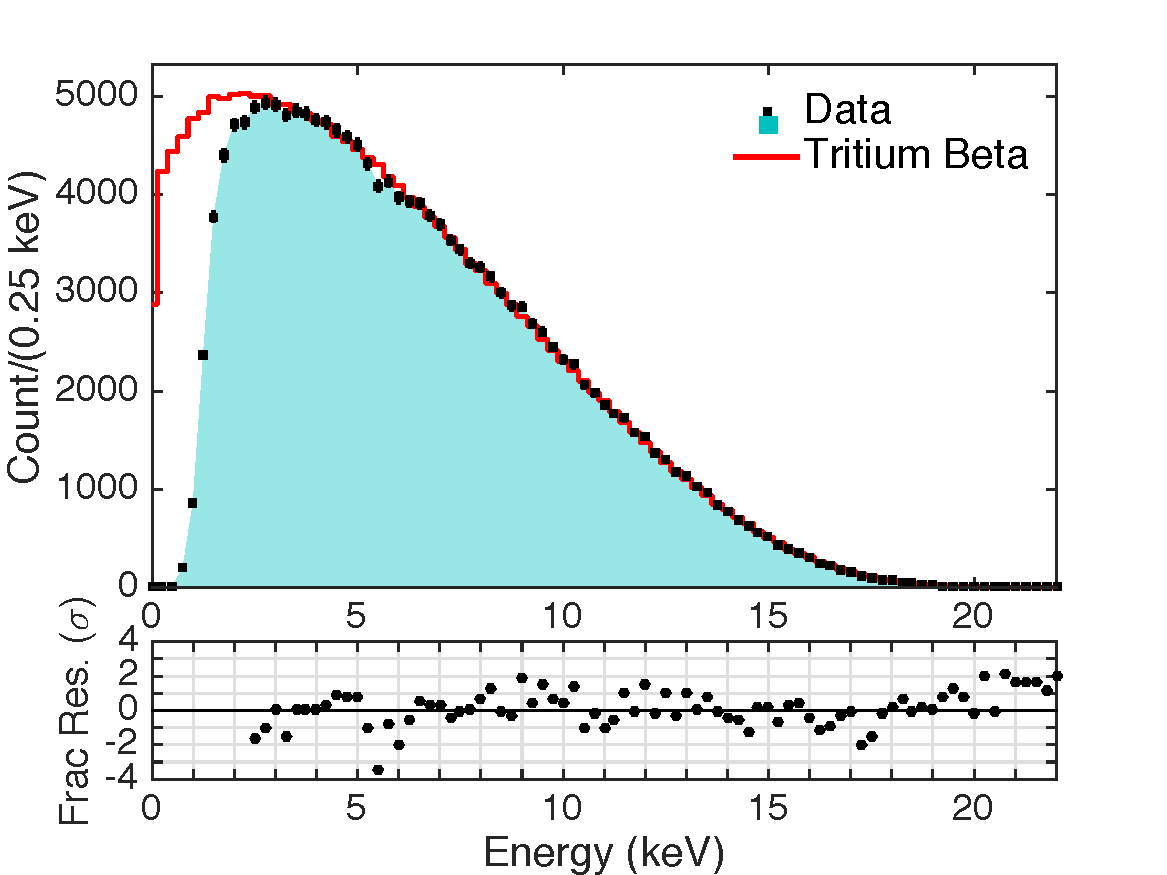
\includegraphics[scale=.425]{TritiumSpectrum.pdf} 
\captionof{figure}{Top: The combined energy spectrum from a high statistics CH$_3$T calibration in LUX.  Data is shown in black, and a model of the expected tritium beta spectrum is shown in red.  Bottom: The residual differences between the data and model for each bin, in units of $\sigma$.}
\label{TritiumSpectrum}
\end{figure}

\begin{figure} [!h]
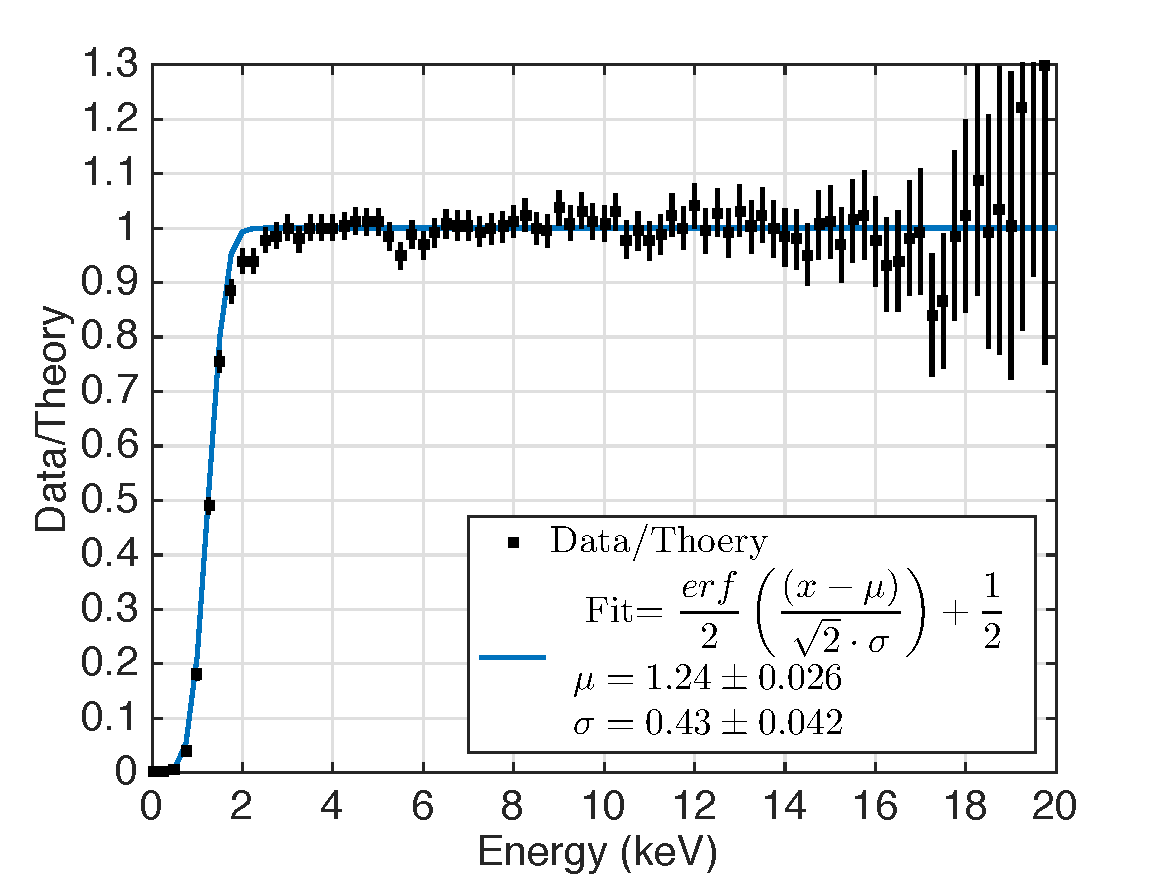
\includegraphics[scale=.4]{TritiumThreshold.pdf} 
\captionof{figure}{The ratio of the tritium data to expectations.  An error function fit used to determine the energy threshold is shown in blue.}
\label{TritiumThreshold}
\end{figure}

The main purpose of the CH$_3$T calibration source is to measure the detector's electron recoil response.  This calibration is crucial when determining the "leakage fraction" of electron recoil backgrounds that fall below the nuclear recoil band mean.  Alternatively, a "discrimination" factor can be defined as the fraction of electron recoil backgrounds that do not fall below the nuclear recoil band mean.  The electron recoil band from a high statistics CH$_3$T calibration is shown in Figure \ref{TritiumERBand}.  The nuclear recoil band calibration from LUX's neutron generator calibration source is also included in Figure \ref{TritumERBand}. These two results have allowed the LUX collaboration to measure the detector's discrimination with unprecedented accuracy.  An average discrimination (1-$f$) for the LUX Run03 result was found to be 99.81\% $\pm$ 0.02\%.

In addition to the calibration results mentioned in this section, the CH$_3$T calibration source has allowed the LUX collaboration to measure fundamental properties of liquid xenon to high accuracy.  These results are discussed in reference \cite{TritiumPaper}.  The calibration source is also an integral part of producing signal corrections in a detector with a nonuniform electric field, a topic which is discussed in chapter \ref{Run04Corrections}.

\newpage 

\begin{figure} [!h]
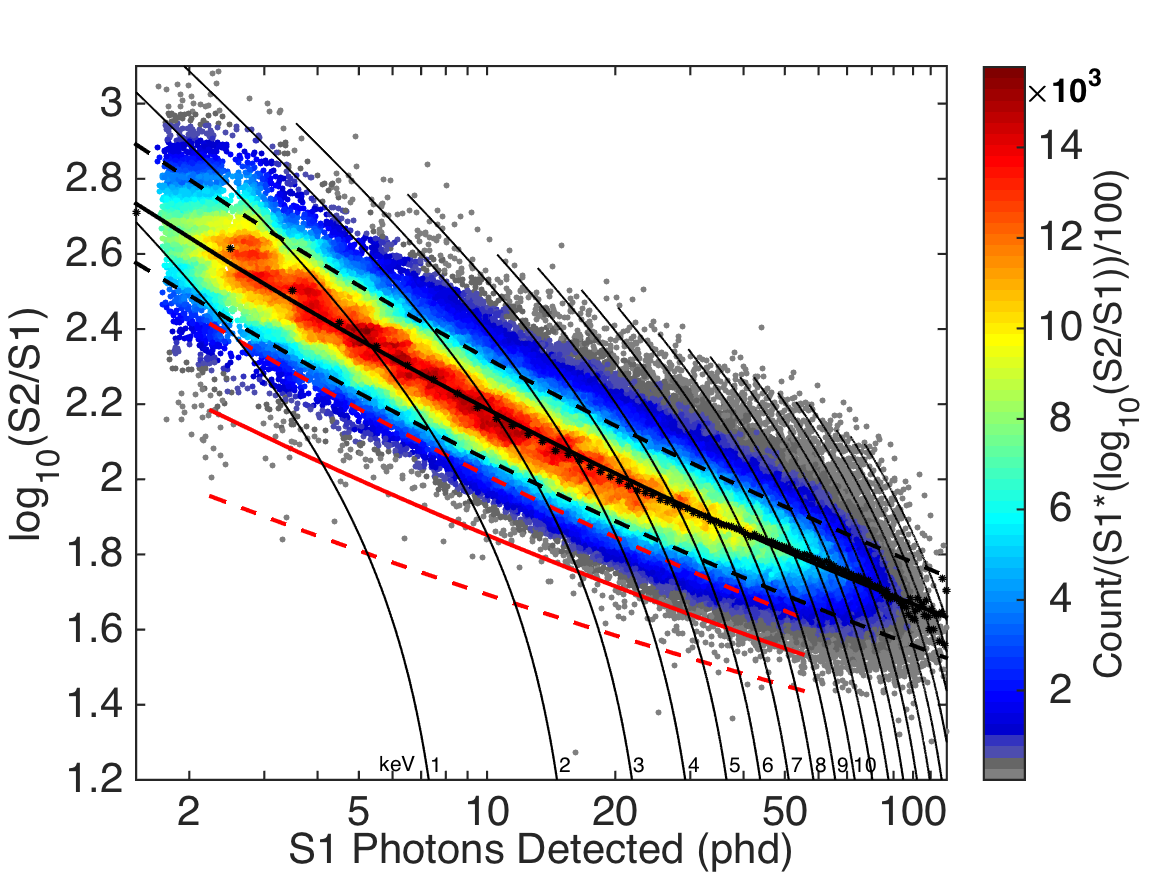
\includegraphics[scale=.35]{TritiumERBand.pdf} 
\captionof{figure}{The electron recoil calibration of LUX resulting from 170,000 CH$_3$T events at 180 V/cm.  The Gaussian means of each S1 bin, as well as power law fits to those means and the 10\% and 90\% contours of the ER band are shown in black.  The power law fits to the mean, 10\%, and 90\% countours of the NR band are shown in red.}
\label{TritiumERBand}
\end{figure}

\begin{figure} [!h]
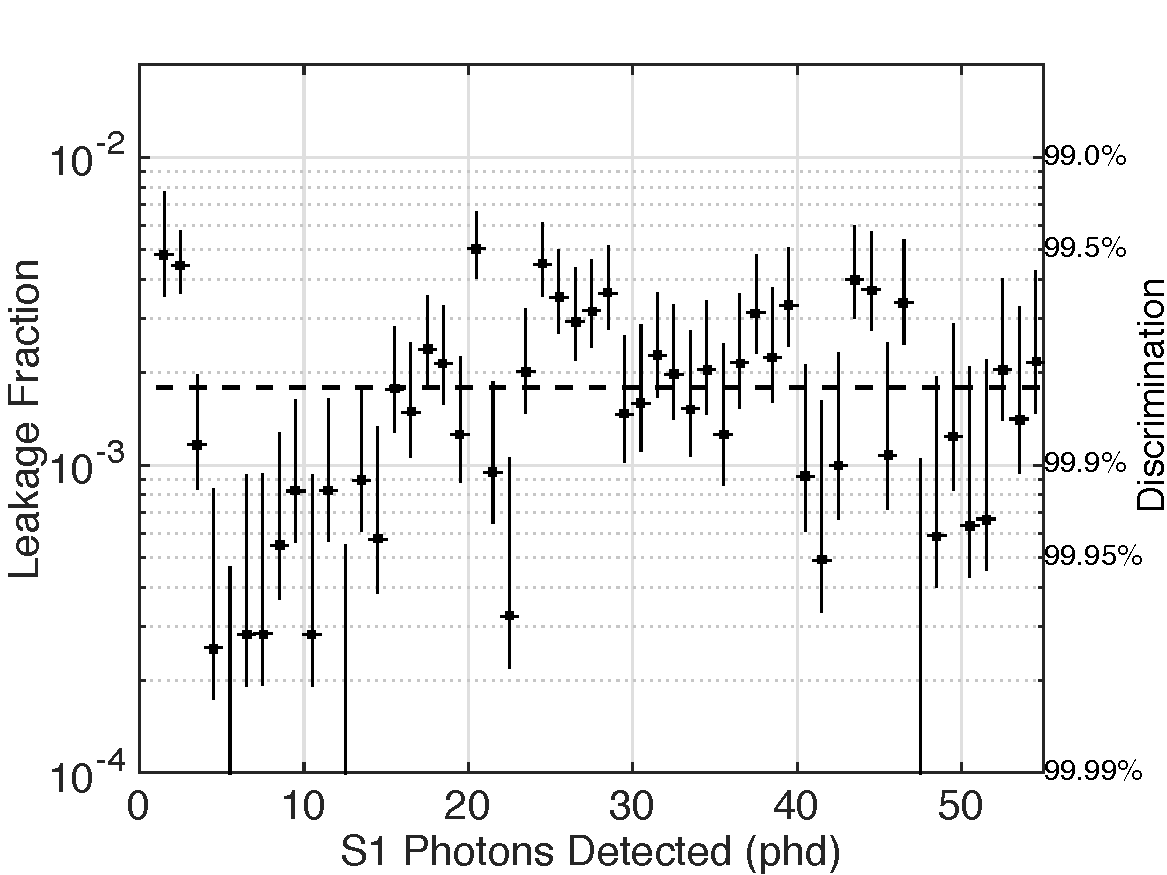
\includegraphics[scale=.35]{TritiumLeakage.pdf} 
\captionof{figure}{The leakage fraction and discrimination versus S1 in the LUX detector at 180 V/cm.}
\label{TritiumLeakage}
\end{figure}


\section{Signal Corrections in the LUX Detector} \label{StandardCalibrations}

In this chapter, we discuss the need for position dependent corrections to the S1 and S2 signals in LUX.  Position dependence in the S1 signal can be introduced by a number of effects.  As photons travel from an interaction site to the PMT arrays they are reflected by teflon panels surrounding the active volume.  The reflectivity of the teflon varies based on the proximity of the interaction site, the angle of incidence of the light, and the surface properties of the teflon.   Photons are also reflected at the liquid xenon surface, causing about two thirds of the S1 signal to be collected in the bottom PMT array.  Events which are closer to the bottom PMT array have more solid angle covered by the PMT array, leading to a larger S1 signal for events toward the bottom of the detector.  A z-dependence of the light collection efficiency can also be introduced by light quenching impurities present in the liquid xenon, although this effect is negligible at the liquid xenon purity levels found in LUX.

As electrons travel from the interaction site to the liquid surface they are absorbed by electronegative impurities in the liquid xenon.  This attenuation of charge leads to a smaller S2 signal from events originating deeper in the detector.  Since the purity of the liquid xenon changes on a weekly basis there is a significant time dependence in the strength of this effect. Small fluctuations in the X-Y plane of the extraction field or the liquid surface level can lead to a position dependence in both the efficiency at which electrons are extracted from the liquid xenon and the number of photoelectrons which are produced per extracted electrons.  Both of these effects are reflected in the size of the S2 signal.  Furthermore, while the individual PMTs are gain matched with LED calibrations, the variation in quantum efficiency between PMTs can lead to an X-Y position dependence in both the S1 and S2 signals.

In the final data analysis, we wish to know the absolute number of photons and electrons produced by recoil interactions, as well as the nuclear recoil discrimination factor at all locations and times in the detector.  It is possible to define position dependent gain factors which convert the S1 signals and S2 signals to number of photons and number of electrons, respectively, but it is more convenient to normalize the S1 and S2 signals to one location in the detector.   Likewise, one could define position and time dependent ER and NR bands to track discrimination over time, but it is more convenient to normalize the data such that the ER band and NR bands are constant at all times and all locations in the detector.  In LUX we choose to normalize the S1 signal to the center of the detector, and the S2 signal to the top of the detector.  The choice to normalize the S1 signal to the center of the detector is arbitrary since the position dependence of the S1 signal has little time dependence, while the choice to normalize the S2 signal to the top of the detector is convenient for circumventing the time dependence inherent at deeper locations in the detector due to varying amount of electron absorbing impurities in the liquid xenon.  Once the S1 and S2 signals are uniform throughout the detector we can define one position independent gain factor for each of the detector signals.  Removing the position dependence of the S1 and S2 signals also results in increased resolution of the S1 and S2 spectra, as well as a narrowing of the ER and NR band widths.


Note that a nonuniform drift field can also introduce position dependence to the S1 and S2 signals.  However, this effect changes the actual number of photons and electrons produced during a recoil interaction, rather than the detector's efficiency of collecting those photons and electrons.  In this chapter we will assume a uniform drift field is present in the detector, and discuss corrections for a detector with a nonuniform electric field in Chapter \ref{Run04Corrections}.

\subsection{Use of $^{83m}$Kr in Signal Corrections}

The LUX detector's $^{83m}$Kr calibration source is an ideal tool to measure corrections for the S1 and S2 signals. A $^{83}$Rb soaked charcoal source is used to inject its $^{83m}$Kr daughter directly into the LUX circulation system.  In the active volume the $^{83m}$Kr decays via internal conversion at 32.1 keV and 9.4 keV with a half life of 1.86 hours.  The half life of the 9.4 keV decay is only 154 ns, causing the two decays to merge into one 41.55 keV pulse in the LUX detector.  Note that it is possible to modify the LUX pulse finder to separate the two S1 signals when desired, but it is nearly impossible to separate the two S2 signals due to diffusion of the electron clouds as they drift to the liquid surface. 

\begin{figure} [!h]
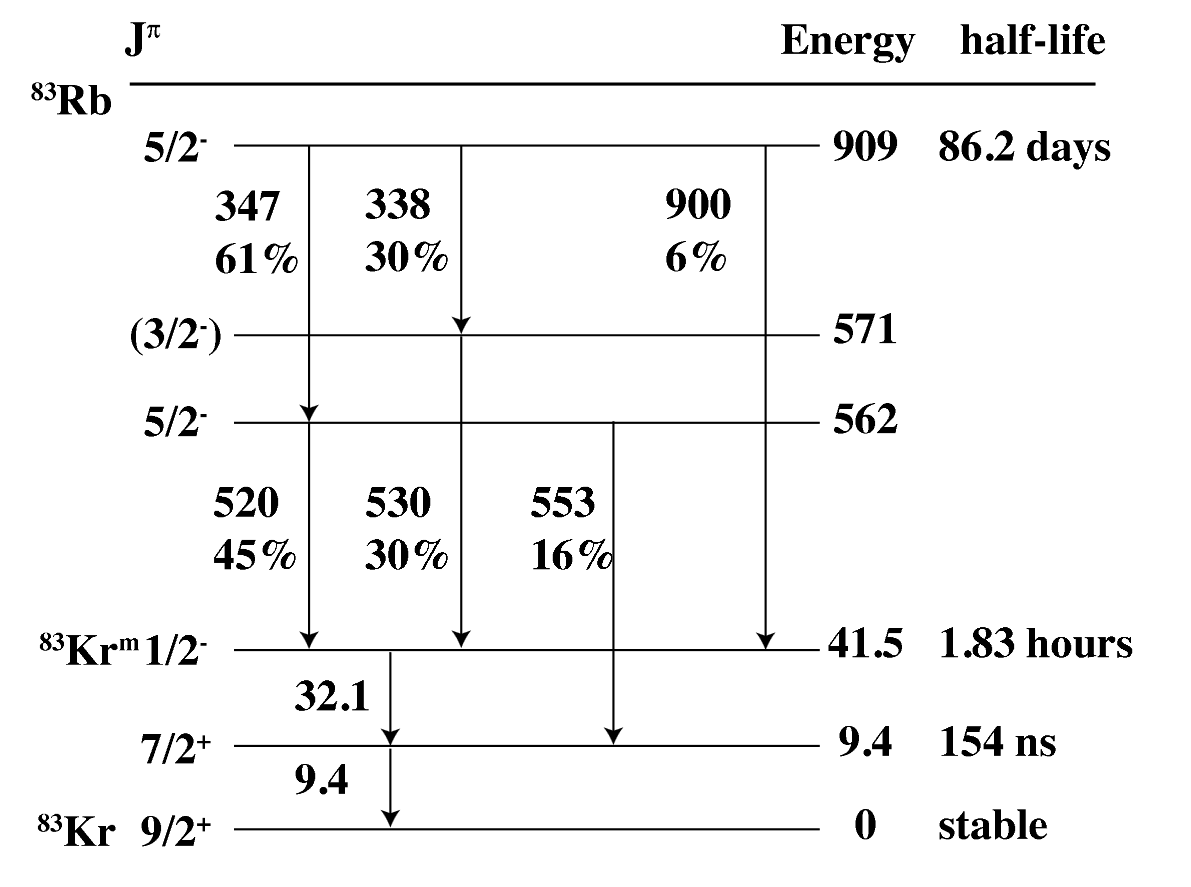
\includegraphics[scale=.35]{Kr83Decay.png} 
\captionof{figure}{The energy level diagram of the $^{83}$Rb and $^{83m}$Kr decays.}
\label{KrDecayScheme}
\end{figure}

Once injected, the $^{83m}$Kr mixes uniformly throughout the active volume in a matter of minutes. The monoenergetic peak of the $^{83m}$Kr events can be measured at any point in the detector to determine the position dependence of the S1 and S2 signals.

\begin{figure} 
\centering
\subfloat{{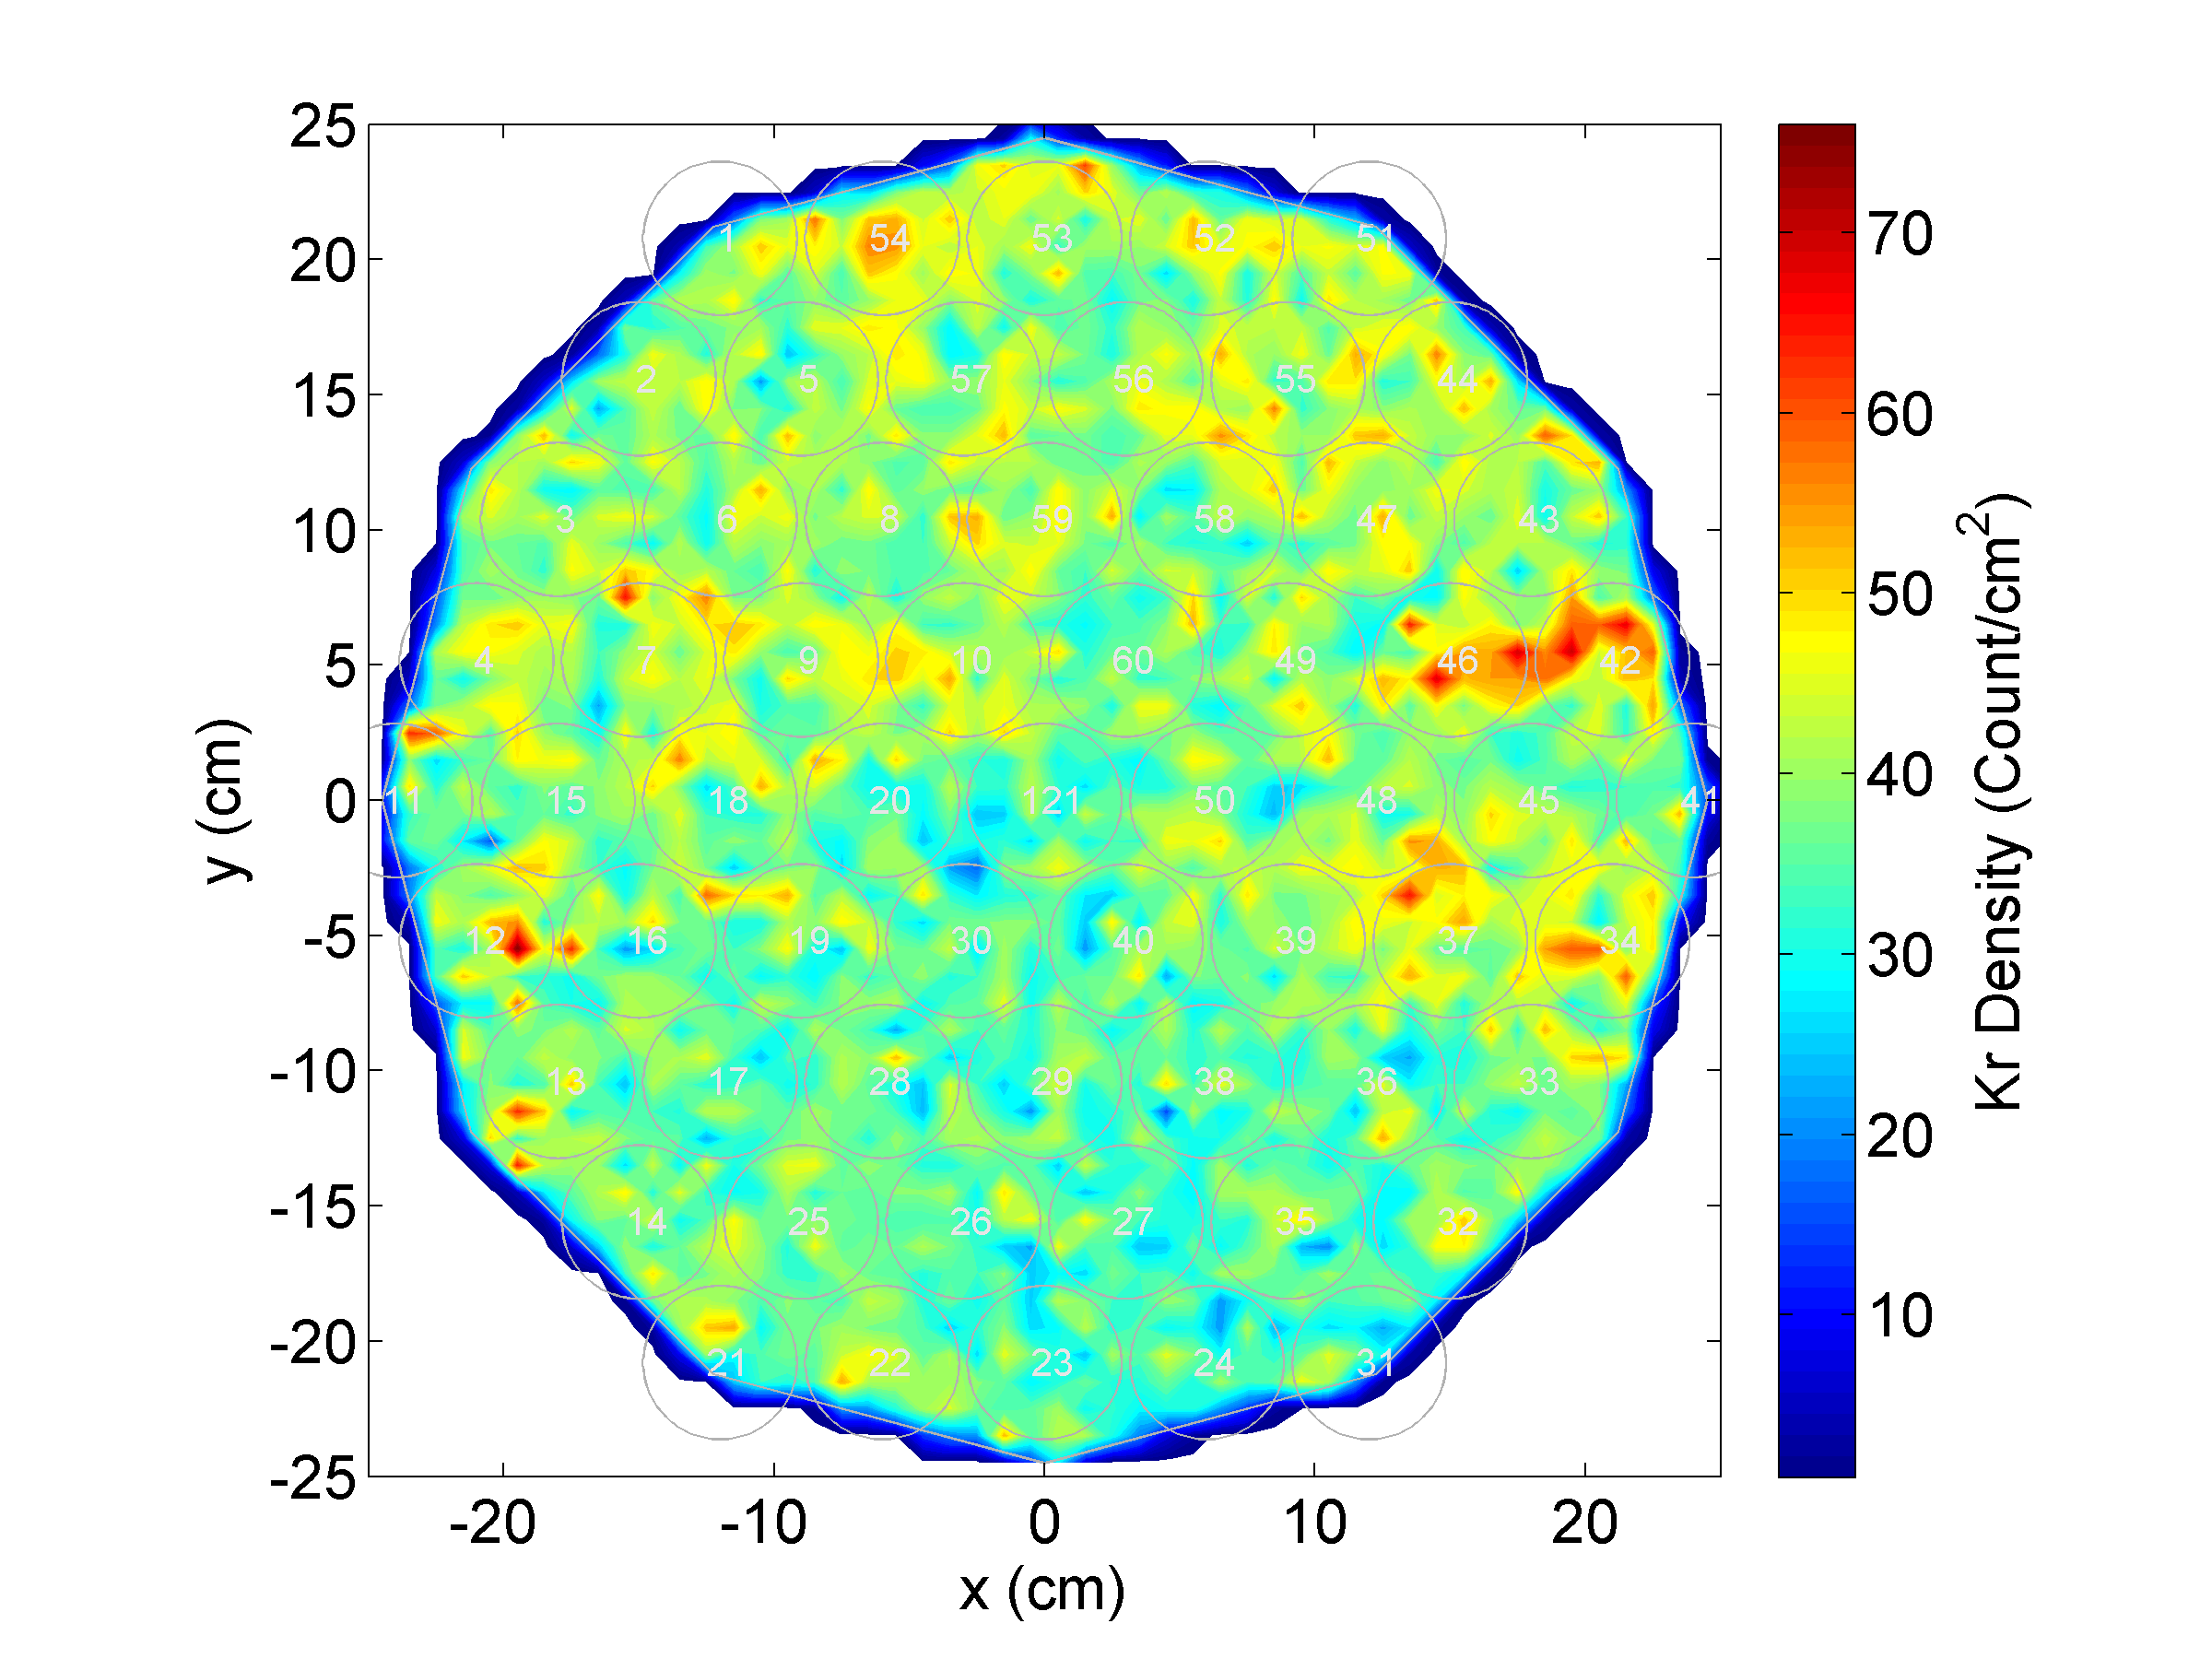
\includegraphics[width=6cm]{KrXvY.png} }}
\qquad
\subfloat{{\includegraphics[width=6cm]{KrR2vz.png} }}
\caption{ (Left) Density of $^{83m}$Kr events in the X-Y plane 10-30 minutes after a $^{83m}$Kr injection. (Right) Density of $^{83m}$Kr events in the R$^2$-Z plane 10-30 minutes after a $^{83m}$Kr injection.}
\label{fig:LandauPlot}
\end{figure}
%Show R^2vZ and XY density plots of Kr for high stats injection in 2015 with time cut of 10-30 minutes to show quick mixing.

The short half life causes the calibration source to be removed from the LUX detector in a matter of hours, allowing for calibration of the S1 and S2 signals on a weekly basis.  This is a crucial property of the calibration source, since the purity of the liquid xenon, and therefore the z-dependence of the S2 signal, changes on a weekly basis.  It is also important that the $^{83m}$Kr is an inert noble gas, a property which prevents temporary attenuation of the S1 and S2 signals during injection of the calibration source. 


\subsection{S1 Corrections}

We first measure the Z dependence of the $^{83m}$Kr S1 pulse areas by slicing the detector into drift time bins with widths defined such that each bin has roughly 300 events.  A Gaussian distribution is fit to the S1 spectra of each bin to determine the location of the spectra means. A second order polynomial is used to determine the S1 Z dependence between and outside of each drift time bin. A detector inefficiency correction for the Z direction is defined by taking the ratio of the S1  pulse area at the center of the detector (defined as $z_c$) to the S1 pulse area as a function of Z as described in the equation
\begin{equation}
\mbox{S}1_{\mbox{z-efficiency-correction}} = \frac{S1(z_c)}{S1(z)}.
\end{equation} 

%Show Run03 S1 gaussian fits and polynomial here -- can get it from the LUG probably
\begin{figure} 
\centering
\subfloat{{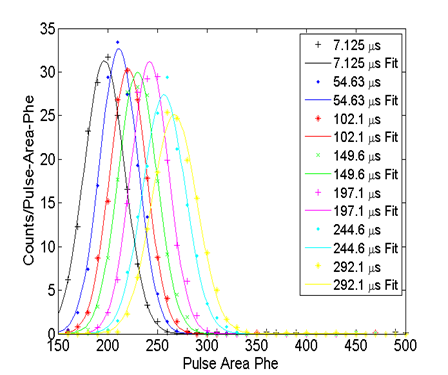
\includegraphics[width=6.3cm]{KrS1_ZDep_Gaussians.png} }}
\qquad
\subfloat{{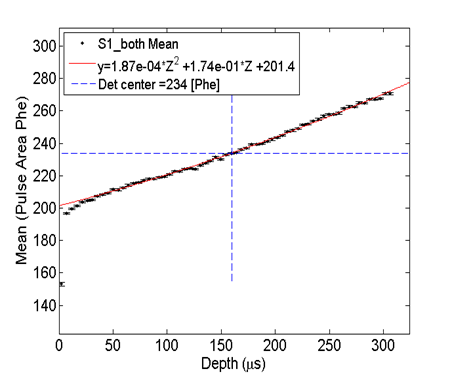
\includegraphics[width=6.3cm]{KrS1_ZDep.png} }}
\caption{ (Left) Gaussian distribution fits to $^{83m}$Kr S1 data that are used to determine the drift time dependence of the S1 pulse area. (Right) The z dependence of the S1 pulse area. Black points indicate the maximum of Gaussian distribution fits for each drift time bin, and red points indicate the polynomial fit to that data.}
\label{fig:KrypCal_S1ZDep}
\end{figure}

The XY dependence of the S1 signal is found by dividing the z-corrected ($S1 \times \mbox{S}1_{\mbox{z-efficiency-correction}}$) data into two dimensional XY bins with lengths defined such that each bin has roughly 300 events, and then fitting Gaussian distributions to the data of each bin.  The mean of the Gaussian distribution from each bin is used to construct S1 XY dependence maps, with a spline interpolation and extrapolation being used to determine the XY dependence between and outside of the bins. (Figure \ref{fig:KrypCalXYDep}) A detector inefficiency correction for the XY direction is defined by taking the ratio of the z-corrected S1 pulse area at the center of the detector to the z-corrected S1 pulse area as a function of XY in cm, as shown below
\begin{align}
\mbox{S}2_{\mbox{xy-efficiency-correction}} &= \frac{\mbox{S}2_{\mbox{z-efficiency-correction}}\times S2(x_c,y_c,z)}{\mbox{S}2_{\mbox{z-efficiency-correction}}\times S2(xyz)}.
\end{align} 
where $x_c$ and $y_c$ are the x and y center of the detector in uncorrected position coordinates.

%Show S1 XY correction here
\begin{figure} 
\centering
\subfloat{{\includegraphics[width=6.3cm]{KrS1_XYDep.png} }}
\qquad
\subfloat{{\includegraphics[width=6.3cm]{KrS1_XYDep_Norm.png} }}
\caption{ (Left) Two dimensional map of the XY dependence in $^{83m}$Kr S1 data determined by fitting a Gaussian distribution to XY bins of the data and tracking the mean of each fit.(Right) Two dimensional map of the XY correction factor which is applied to z-corrected S1 data.}
\label{fig:KrypCalS1XYDep}
\end{figure}


When enough stats are present in a $^{83m}$Kr calibration data set, a three dimensional S1 corrections map is favored over the two step (Z, then XY) corrections described above.  In this case, the uncorrected S1 data is divided into three dimensional XYZ voxels with volumes defined such that each bin has roughly 300 events. A Gaussian distribution is fit to the data of each voxel, and the mean of the Gaussian distribution is used to construct three dimensional S1 dependence maps, with a spline interpolation and extrapolation being used to determine the XYZ dependence between and outside of the voxel. (Figure \ref{fig:KrypCalXYDep}) A three dimensional detector inefficiency correction is then defined by taking the ratio of the uncorrected S1 pulse area at the center of the detector to uncorrected S1 pulse area as a function of X,Y, and drift time, as shown below
\begin{align}
\mbox{S}1_{\mbox{xyz-efficiency-correction}} &= \frac{S1(x_c,y_c,z_c)}{S1(xyz)}.
\end{align} 
The detector inefficiency effects in the S1 signal are all due to the unchanging internal geometry of the detector.  Therefore, the S1 correction maps vary by only a few percent over time and a single high stats three dimensional correction map can be applied to data over a long period of time.  

Write formula for the actual S1 corrected data here. DO THIS!!

Improvement in S1 resolution - resolution improves by 5\%, mean shifts by 2\% (absolute, not relative)

\begin{figure} [!h]
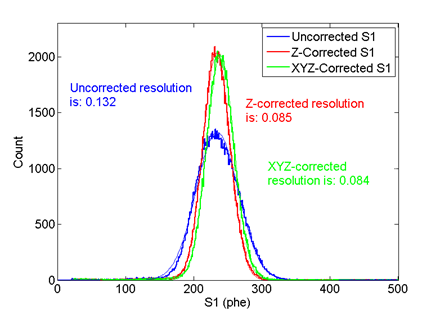
\includegraphics[scale=.75]{KRS1_ResolutionImprovement.png} 
\captionof{figure}{The $^{83m}$Kr S1 spectrum with no corrections applied (blue), z dependent corrections applied (red), and xyz dependent corrections applied (green).}
\label{KrS1Improvement}
\end{figure}


Stability in S1 over time. Corrected S1 varies by ~0.6\% over time.  Discrete jump is due to change in S1 corrections map

\begin{figure} [!h]
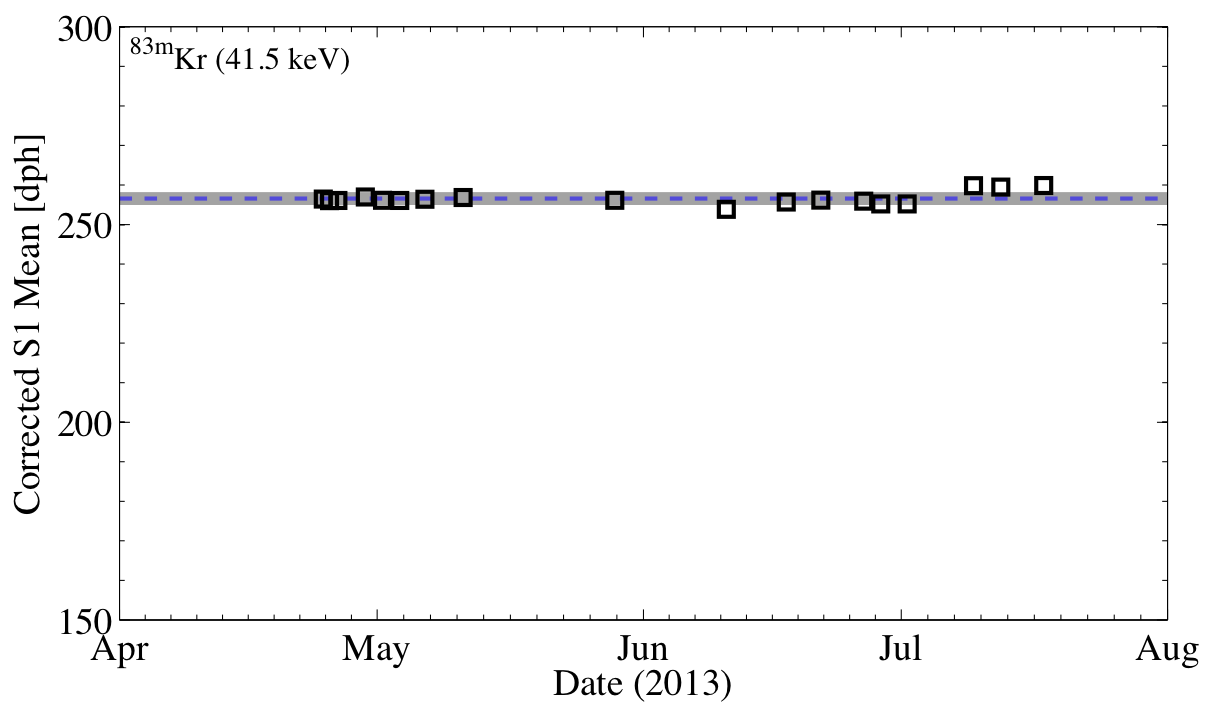
\includegraphics[scale=.35]{CorrectedS1_Stability.png} 
\captionof{figure}{The corrected $^{83m}$Kr S1 mean over the duration of LUX's Run03 data taking campaign.}
\label{KrS2Stability}
\end{figure}

\subsection{S2 Corrections}

As with the S1 signal, we measure the Z dependence of the $^{83m}$Kr S2 pulse areas by slicing the detector into drift time bins with widths defined such that each bin has roughly 300 events. 
An exponential decay is fit to the drift time dependence of the mean of each $^{83m}$Kr S2 distribution.  A detector inefficiency correction for the Z direction is defined by taking the ratio of the S2  pulse area just below the liquid surface to the S2 pulse area as a function of Z as described in the equation
\begin{equation}
\mbox{S}2_{\mbox{z-efficiency-correction}} = \frac{S2(z=0)}{S2(z)}.
\end{equation} 

%Show S2 Gaussian fits and exponential fit here -- can probably get it from LUG
\begin{figure} 
\centering
\subfloat{{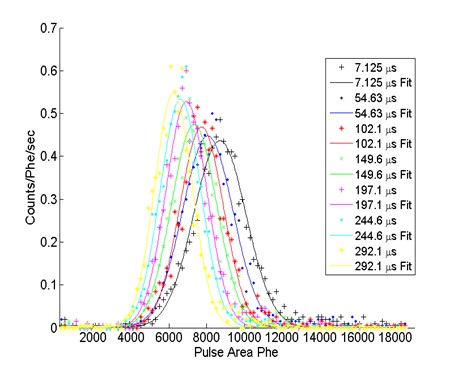
\includegraphics[width=6.3cm]{KrS2_ZDep_Gaussians.png} }}
\qquad
\subfloat{{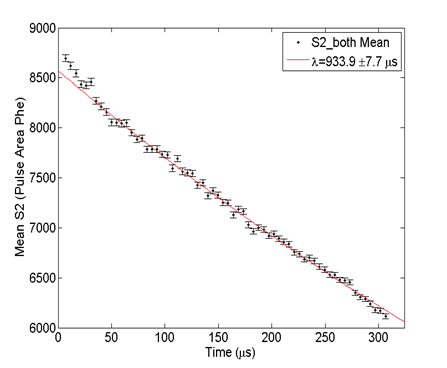
\includegraphics[width=6.3cm]{KrS2_ZDep.png} }}
\caption{ (Left) Gaussian distribution fits to $^{83m}$Kr S2 data that are used to determine the drift time dependence of the S2 pulse area. (Right) The z dependence of the S2 pulse area. Black points indicate the maximum of Gaussian distribution fits for each drift time bin, and red points indicate the exponential fit to that data.}
\label{fig:KrypCal_S2ZDep}
\end{figure}

The process of measuring the XY dependence of the S2 signal is identical to the process of measuring the XY dependence of the S1 signal.  The z-corrected ($S2 \times \mbox{S}2_{\mbox{z-efficiency-correction}}$ S2 data is divided into two dimensional XY bins with lengths defined such that each bin has roughly 300 events, and a Gaussian distribution is fit to the data of each bin.  The mean of the Gaussian distribution from each bin is used to construct S2 XY dependence maps, with a spline interpolation and extrapolation being used to determine the XY dependence between and outside of the bins. (Figure \ref{fig:KrypCalXYDep}) A detector inefficiency correction for the XY direction is defined by taking the ratio of the z-corrected S2 pulse area at the center of the detector to the z-corrected S2 pulse area as a function of XY in cm, as shown below
\begin{align}
\mbox{S}2_{\mbox{xy-efficiency-correction}} &= \frac{\mbox{S}2_{\mbox{z-efficiency-correction}}\times S2(x_c,y_c,z)}{\mbox{S}2_{\mbox{z-efficiency-correction}}\times S2_(xyz)}.
\end{align} 
where $x_c$ and $y_c$ are the x and y center of the detector in uncorrected position coordinates.

%Show S2 XY correction here
\begin{figure} 
\centering
\subfloat{{\includegraphics[width=6.3cm]{KrS2_XYDep.png} }}
\qquad
\subfloat{{\includegraphics[width=6.3cm]{KrS2_XYDep_Norm.png} }}
\caption{ (Left) Two dimensional map of the XY dependence in $^{83m}$Kr S2 data determined by fitting a Gaussian distribution to XY bins of the data and tracking the mean of each fit.(Right) Two dimensional map of the XY correction factor which is applied to z-corrected S2 data.}
\label{fig:KrypCalS2XYDep}
\end{figure}

The z-dependence of the S2 signal is a function of the liquid xenon purity.  TALK ABOUT FORMULA FOR ELECTRON LIFETIME HERE. Therefore, the S2 correction maps vary significantly over time and must be remeasured on a weekly basis.  To apply S2 efficiency corrections to data at any time, a weighted average of the $^{83m}$Kr S2 Z dependence is used to defined a time interpolated S2 Z dependence correction.  
Write formula for the actual S2 corrected data here.

%Show lifetime plots from Run03 here
\begin{figure} [!h]
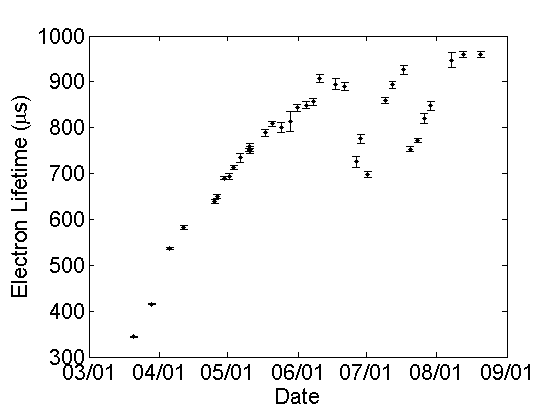
\includegraphics[scale=.75]{LUX_eLifetime_Run03.png} 
\captionof{figure}{The electron lifetime over the duration of LUX's Run03 data taking campaign.}
\label{KrS2Improvement}
\end{figure}

Improvement in S2 resolution - improves by 4\% and shifts by 21\% (absolute, not relative)

\begin{figure} [!h]
\includegraphics[scale=.75]{KRS2_ResolutionImprovement.png} 
\captionof{figure}{The $^{83m}$Kr S2 spectrum with no corrections applied (blue), z dependent corrections applied (red), and xyz dependent corrections applied (green).}
\label{KrS2Improvement}
\end{figure}

Stability in S2 over time  The corrected corrected S2 varies by ~2\% over time.

\begin{figure} [!h]
\includegraphics[scale=.35]{CorrectedS2_Stability.png} 
\captionof{figure}{The corrected $^{83m}$Kr S2 mean over the duration of LUX's Run03 data taking campaign.}
\label{KrS2Stability}
\end{figure}

\subsection{Resolution as a measure of Electron Lifetime}

\subsection{Radon as a measure of Electron Lifetime}

\subsection{A PMT-by-PMT approach to S1 Corrections}


\section{Energy Scale Calibrations} \label{CombinedEnergyModel}

%Discuss recombination physics and the ability to turn the now (emphasis on this, since it is how we transition from the previous section) corrected data into an combined energy scale.  Then basically cover recombination physics (prob in Attila's thesis) and Doke plot from my Doke plot write up.

\subsection{Recombination Physics} \label{RecombSec} 
\subsection{Doke Plot}
\subsection{Tritium Chi2 Method}


\section{Calibration of the LUX Detector in a nonuniform Field} \label{Run04Corrections}

%Put the LUX Run04 KrypCal note here...

\subsection{Source of nonuniform Field}
\subsection{Issues arising from nonuniform Field}
\subsection{Removing field effects from data with theory}
\subsection{Removing field effects from data with Monte Carlo}
\subsection{Electron Recoil Calibration in a nonuniform Field}


\begin{thebibliography}{1}

\bibitem{Zwicky} Zwicky.  \emph{Helv. Phys. Acta} 6:110 (1933)
\bibitem{Persic} Persic, Salucci, Stel.  \emph{Mon. Not. R. Astron. Soc.} 281:27 (1996)
\bibitem{Battaner} Battaner, Florido.  \emph{Fund. Cosmic Phys.} 21:1 (2000)
\bibitem{Binney} Binney, Tremaine. \emph{Galactic Dynamics}. Princeton, NJ: Princeton Univ. Press (1988)
\bibitem{Javorsek} Javorsek II, Fischbach. \emph{The Astrophysical Journal} 568:1-8 (2002)
\bibitem{EROS} EROS Collab.  \emph{Astron. Astrophys.} 400:951 (2003)
\bibitem{Alcock} Alcock, et al. (MACHO collab.)  \emph{Ap. J.} 542:281 (2000)
\bibitem{Tytler} Tytler, et al. \emph{Ap. J.} 617:1-28 (2004)
\bibitem{Spergel} Spergel, et al. \emph{Ap. J. Suppl.} 148:175 (2003)
\bibitem{Robertson} Robertson. \emph{J. Phys.:Conf. Ser.} 173:012016 (2009)
\bibitem{Parke} Parke.  \emph{FERMILAB-CONF-06-248-T} (2006)
\bibitem{Pastor} Pastor.  \emph{Physics of Particles and Nuclei} 42(4):628-640 (2012)
\bibitem{Kolb} Kolb, Turner. \emph{The Early Universe}.  Cambridge, MA: Perseus (1994)
\bibitem{Jungman} Jungman, Kamionkowski, Griest.  \emph{Phys. Rep.} 267:195 (1996)
\bibitem{Goldberg} Goldberg.  \emph{Phys. Rev. Lett.} 50:1419 (1983)
\bibitem{Ellis} Ellis, et al. Nucl. \emph{Phys. B} 238:453 (1984)
\bibitem{Bennett} Bennett, et al. \emph{Ap. J. Suppl.} 148:1 (2003)
\bibitem{Arnowitt} Arnowitt, Dutta, Hu. \emph{Beyond The Desert '03}, Castle Ringberg, Germany (June 2003), hep-ph/0310103
\bibitem{Roszkowski} Roszkowski.  \emph{Pramana} 62:1 (2004) hep-ph/0404052
\bibitem{Baluni} Baluni. \emph{Phys. Rev. D} 19, 2227 (1979)
\bibitem{Chung} Chung, et al.  \emph{Phys. Rev. D} 59:023501 (1999) arXiv:hep-ph/9802238
\bibitem{Goodman} Goodman, Witten. \emph{Phys. Rev. D} 31:3059 (1985)
\bibitem{Lewin} Lewin, Smith. \emph{Astropart. Phys.} 6:87 (1996)
\bibitem{Shan} Shan. \emph{JCAP} 1107:005 (2011)
\bibitem{Gaitskell} Gaitskell.  \emph{Annu. Rev. Nucl. Part. Sci.} 54:315-359 (2004)
\bibitem{McKinsey} McKinsey, et al.  \emph{Journal of Physics: Conference Series} 203:012026 (2010) 
\bibitem{Fiorucci} Fiorucci, et al.  \emph{AIP Conference Proceedings} 1200:977 (2010)
\bibitem{Kastens} Kastens, et al. \emph{Phys. Rev. C} 80:045809 (2009)

\bibitem{D'Amico} D'Amico, Guido, et al. arXiv:0907.1912[astro-ph.CP] 
\bibitem{Wu} Wu, et al.  \emph{Monthly Notices of the Royal Astronomical Society} 301(3):861-971.  arXiv:astro-ph/9808179
\bibitem{Griest} Griest, et al.  \emph{Phys. Rept.} 333:167-182 (2000) 
\bibitem{Aprile} E. Aprile, T.Doke. \emph{Rev. Mod. Phys.} 82:2053-2097 (2010)
\bibitem{Miyake} Miyake, et al.  \emph{J. vac. Sci. technol. A.} 1:1446-1451 (1983)
\bibitem{Piche} R. Piche. \emph{Partial Differential Equations} Tampere University of Technology.
\bibitem{ComaZ} B. Ryden, "Introduction to Cosmology," San Francisco, USA: Addison-Wesley (2003).
\bibitem{Paradijs} Paradijs J, Bleeker J. X-Ray Spectroscopy in Astrophysics. Springer (1999) Page 33
\bibitem{Vikhlinin}
Vikhlinin A, et al. Chandra Sample of Nearby Relaxed Galaxy Clusters: Mass, Gas Fraction, And Mass-Temperature Relation.  Astrophys. J. 640 (2006) 691-709. Jul 2005. arXiv:astro-ph/0507092
\bibitem{Bin-Nun} Bin-Nun, Amitai Yisrael, “Gravitational Lensing with a Large Deflection Angle as a Probe of General Relativity and the Galactic Center” (2010). Publicly accessible Penn Dissertations. Paper 252.
\bibitem{Xiang} Wu, Xiang-Ping, A comparison of different cluster mass estimates: consistency of discrepancy? (1998)

%@article{Wu:1998ju,
%      author         = "Wu, Xiang-Ping and Chiueh, Tzihong and Fang, Li-Zhi and
 %                       Xue, Yan-Jie",
  %    title          = "{A comparison of different cluster mass estimates:
   %                     consistency or discrepancy ?}",
  %    journal        = "Mon. Not. Roy. Astron. Soc.",
  %    volume         = "301",
  %    year           = "1998",
  %    pages          = "861",
  %    doi            = "10.1046/j.1365-8711.1998.02055.x",
  %    eprint         = "astro-ph/9808179",
  %    archivePrefix  = "arXiv",
  %    primaryClass   = "astro-ph",
  %    SLACcitation   = "%%CITATION = ASTRO-PH/9808179;%%"
%}

\bibitem{Schneider} Schneider, P. Extragalactic Astronomy and Cosmology: An Introduction. Berlin: Springer. (2006)

\bibitem{Pires} Pires, S, et al.  Light on Dark Matter with Weak Gravitational Lensing. (2009)  	arXiv:0908.4157


%@MISC{Pires_lighton,
%    author = {S. Pires and J. -l. Starck and A. Réfrégier},
%    title = {LIGHT ON DARK MATTER WITH WEAK GRAVITATIONAL LENSING 1 Light on Dark Matter with Weak %Gravitational Lensing},
%    year = {}
%}

\bibitem{Refregier} Refregier, A. Weak Gravitational Lensing by Large-Scale Structure.  Annual Reviews of Astronomy and Astrophysics.  (2003) 41:645-668

\bibitem{Clowe} Clowe, et al.  A Direct Empirical Proof of the Existence of Dark Matter.  Astrophys. J. 648:L109-L113. (2006)  	arXiv:astro-ph/0608407

\bibitem{Kurki-Suonio} Kurki-Suonio, Cosmological Perturbation Theory. (2015) http://theory.physics.helsinki.fi/~cpt/Cosmo12.pdf

\bibitem{Whu} Hu. CMB Introduction.  (2001) background.uchicago.edu/~whu/intermediate/map1.html

\bibitem{Planck} Plank Collaboration.  Planck 2013 Results.   	A\&A 571, A15 (2014)	arXiv: 	arXiv:1303.5075

\bibitem{Begeman} Begeman, Broeils, and Sanders, 1991, MNRAS, 249, 523

\bibitem{Fermi-LAT} Fermi-LAT Collaboration.  Fermi LAT Search for Dark Matter in Gamma-ray Lines and the Inclusive Photon Spectrum. (2012) arXiv:1205.2739

\bibitem{Knapp} Knapp, et al.  Extensive Air Shower Simulations at the Highest Energies.  Astropart. Phys. 19 (2003) 77. arXiv:astro-ph/0206414

\bibitem{HESS} The H.E.S.S. Collaboration.  Search for a Dark Matter annihilation signal from the Galactic Center halo with H.E.S.S. Phys.Rev.Lett.106:161301 (2011)  	arXiv:1103.3266

\bibitem{VERITAS} The VERITAS Collaboration. The VERITAS Dark Matter Program. (2013) arXiv:1303.1406 

\bibitem{IceCube} IceCube Collaboration. Search for dark matter annihilations in the Sun with the 79-string IceCube detector. Phys. Rev. Lett. 110, 131302 (2013) arXiv:1212.4097 

\bibitem{IceCube2} IceCube Collaboration. IceCube Search for Dark Matter Annihilation in nearby Galaxies and Galaxy Clusters. Phys. Rev. D88 (2013) 122001 arXiv:1307.3473

\bibitem{Cheng}  H. C. Cheng, J. L. Feng and K. T. Matchev, Phys. Rev. Lett.89, 211301 (2002) [arXiv:hep-ph/0207125].

\bibitem{Kamionkowsk} M. Kamionkowski and M. S. Turner, Phys. Rev. D
43, 1774 (1991).

\bibitem{Stecker} Stecker, F. W. 1970, Ap\&SS, 6, 377

\bibitem{PEBS} PEBS Collaboration.   %http://www1b.physik.rwthaachen.de/~pebs/?PEBS_physics:Positron_fraction

\bibitem{FermiPositron} The Fermi LAT Collaboration, Measurement of Separate Cosmic-Ray Electron and Positron Spectra with the Fermi Large Area Telescope, Phys.Rev.Lett. 108 (Jan., 2012) 011103, [arXiv:1109.0521].

\bibitem{PamelaPositron} PAMELA Collaboration.  The cosmic-ray positron energy spectrum measured by PAMELA.  Phys. Rev. Lett. 111 (2013) 081102  	arXiv:1308.0133 

\bibitem{AMSPositron} The AMS Collaboration, High statistics measurement of the positron fraction in primary cosmic rays of 0.5-500 gev with the alpha magnetic spectrometer on the international space station, Phys. Rev. Lett.113(Sep, 2014) 121101

\bibitem{Serpico} P. Serpico. Astrophysical models for the origin of the positron "excess". 10.1016/j.astropartphys.2011.08.007  	arXiv:1108.4827

\bibitem{Bertone} Bertone, et al. Particle Dark Matter: Evidence, Candidates and Constraints. Phys.Rept.405:279-390,2005 arXiv:hep-ph/0404175

\bibitem{Beltran} Beltran, et al.  Maverick dark matter at colliders.  JHEP 1009:037,2010 arXiv:1002.4137

\bibitem{ATLAS} The ATLAS Collaboration. Search for dark matter candidates and large extra dimensions in events with a jet and missing transverse momentum with the ATLAS detector. JHEP 1304 (2013) 075 arXiv:1210.4491 

\bibitem{Lewin}  D Lewin and P F Smith.  Review of mathematics, numerical factors, and
corrections for dark matter experiments based on elastic nuclear recoil.
Astroparticle Physics, 1996.

\bibitem{PauloThesis} P Br\'as. Finding a needle in a haystack: Background studies and WIMP detection efficiency in LUX. (2015)

\bibitem{LuxDetector} D Akerib, et al.  The Large Underground Xenon (LUX) Experiment.  http://arxiv.org/pdf/1211.3788v2.pdf

\bibitem{BradleyThesis} A Bradley. LUX Thermosyphon Cryogenics and Radon-Related Backgrounds for the First WIMP Result. %http://teacher.pas.rochester.edu:8080/wiki/pub/Lux/LuxRequiredReading/AWB_PhDThesis_20140120.pdf

\bibitem{JonOutgassing} J Balajthy, and C Hall. Simulations of CH3T Diffusion into Plastic Parts of the LUX Detector. LUX Document Database. (2013) http://teacher.pas.rochester.edu:8080/wiki/pub/Lux/LuxDB00000481

\bibitem{JonOutgassingTwo} J Balajthy.  Results of the Large CH4 Injection from April 2015.  LUX Document Database. (2015) http://teacher.pas.rochester.edu:8080/wiki/bin/view/Lux/LuxDB00000445

\bibitem{TritiumPaper} D Akerib et al.  Tritium calibration of the LUX dark matter experiment.  	Phys. Rev. D 93, 072009 (2016)  http://arxiv.org/abs/1512.03133

\end{thebibliography}


\end{document}

